%TODO Go through appendix and check which models are still missing
%% norway matching
%% norway terciles
%% full coefficient print
% check all results are the same as in original draft
% remove unnecessary comments from appendix

\documentclass[12pt]{article}
% Packages
\usepackage[utf8]{inputenc}
\usepackage[T1]{fontenc}
\usepackage[margin=1in]{geometry}
\usepackage[UKenglish]{babel}% http://ctan.org/pkg/babel
\usepackage[UKenglish]{isodate}% http://ctan.org/pkg/isodate
\usepackage{amsmath, amsthm, amsfonts, amssymb}
\usepackage{mathrsfs}           % \mathscr font.
\usepackage{setspace}
\usepackage[colorlinks=true,
    linkcolor=red,
    citecolor=red,
    urlcolor=red,
    breaklinks]{hyperref}
\usepackage{graphicx}
\usepackage{booktabs}
\usepackage{subcaption}
\usepackage{xcolor}
% \usepackage[style = authoryear, autocite=inline, doi=false,isbn=false,url=false]{biblatex}
\usepackage{natbib}
% \usepackage{libertine}

% \usepackage[sf]{titlesec} % make section headings \sffamily

% Header styling
% make headers \sffamily
% \newpagestyle{main}[\sffamily]{
%     \sethead{\thepage}{}{\sectiontitle}
%     }
% \pagestyle{main}
\usepackage{titling}
% make titling elements \sffamily
% \pretitle{\begin{center}\sf \LARGE}
% \preauthor{\begin{center}
%             \large \lineskip 0.5em%
%             \begin{tabular}[t]{c}}
% \predate{\begin{center}\large}
\usepackage{abstract}
% make abstract title \sffamily
% \titleformat{\section}[block]{\Large \bf \sffamily}{\thesection}{1em}{}
\usepackage{caption}
\captionsetup{labelfont = bf}

\usepackage{longtable}
\usepackage{dcolumn}
\usepackage[toc,page,header]{appendix}
\usepackage{minitoc}
\usepackage{booktabs}
\usepackage{longtable}
\usepackage{array}
\usepackage{multirow}
\usepackage{wrapfig}
\usepackage{float}
\usepackage{colortbl}
\usepackage{pdflscape}
\usepackage{tabu}
\usepackage{threeparttable}
\usepackage{flafter}
\usepackage{threeparttablex}
\usepackage[normalem]{ulem}
\usepackage{makecell}
\usepackage{xcolor}
\usepackage{color, colortbl}
\definecolor{lgrey}{gray}{0.9}
\usepackage{siunitx}
\sisetup{
    detect-all,
    round-integer-to-decimal = true,
    group-digits             = true,
    group-minimum-digits     = 4,
    group-separator          = {\,},
    table-align-text-pre     = false,
    table-align-text-post    = false,
    input-signs              = + -,
    input-symbols            = {*} {**} {***},
    input-open-uncertainty   = ,
    input-close-uncertainty  = ,
    retain-explicit-plus,
    parse-numbers = false
}
\newcolumntype{d}[1]{D..{#1}}


\usepackage{etoolbox}

\makeatletter

% Patch case where name and year are separated by aysep
% \patchcmd{\NAT@citex}
%   {\@citea\NAT@hyper@{%
%      \NAT@nmfmt{\NAT@nm}%
%      \hyper@natlinkbreak{\NAT@aysep\NAT@spacechar}{\@citeb\@extra@b@citeb}%
%      \NAT@date}}
%   {\@citea\NAT@nmfmt{\NAT@nm}%
%    \NAT@aysep\NAT@spacechar\NAT@hyper@{\NAT@date}}{}{}

% % Patch case where name and year are separated by opening bracket
% \patchcmd{\NAT@citex}
%   {\@citea\NAT@hyper@{%
%      \NAT@nmfmt{\NAT@nm}%
%      \hyper@natlinkbreak{\NAT@spacechar\NAT@@open\if*#1*\else#1\NAT@spacechar\fi}%
%        {\@citeb\@extra@b@citeb}%
%      \NAT@date}}
%   {\@citea\NAT@nmfmt{\NAT@nm}%
%    \NAT@spacechar\NAT@@open\if*#1*\else#1\NAT@spacechar\fi\NAT@hyper@{\NAT@date}}
%   {}{}

\makeatother

% Define symbols and maths shortcuts
\DeclareRobustCommand{\bbone}{\text{\usefont{U}{bbold}{m}{n}1}}
\DeclareMathOperator{\EX}{\mathbb{E}} % expected value
\DeclareMathOperator{\V}{\mathbb{V}}
\DeclareMathOperator{\Prob}{\mathbb{P}}
\newcommand*{\trans}{^{\mathsf{T}}} %matrix transpose



\usepackage{booktabs}
\usepackage{longtable}
\usepackage{array}
\usepackage{multirow}
\usepackage{wrapfig}
\usepackage{float}
\usepackage{colortbl}
\usepackage{pdflscape}
\usepackage{tabu}
\usepackage{threeparttable}
\usepackage{threeparttablex}
\usepackage[normalem]{ulem}
\usepackage{makecell}
\usepackage[toc,page,header]{appendix}
\usepackage{xcolor}
\usepackage{siunitx}
\usepackage{chngcntr}
\usepackage{minitoc}
\usepackage{caption}
\usepackage{setspace}
\usepackage[hang]{footmisc}
\captionsetup{font = small}

% Make the "Part I" text invisible
\renewcommand \thepart{}
\renewcommand \partname{}

\setlength\labelsep{0pt}

\title{The Gender Gap in Political Careers \\ Under Proportional Representation}
\date{April 2023}
\date{}
\author{Tobias Nowacki\thanks{Senior Data Scientist, Deliveroo. I thank Kirk Bansak, Chris Berry, Gary Cox, Andy Eggers, Jon Fiva, Olle Folke, Ignacio Lago, Justin Grimmer, Andy Hall, Apoorva Lal, Sandy Handan-Nader, Jens Hainmueller, Jonathan Rodden, Brett Parker, Tine Paulsen, Soledad Prillaman, Johanna Rickne, Dan Smith, Dan Thompson, and participants in the Democracy and Polarization Lab and at the APSA 2021 panel for helpful comments.}}

% \addbibresource{Spain_Careers.bib}


% Begin Document
\begin{document}

%
% FRONT PAGE -----------------------------------------------------------------
%

\renewcommand \thepart{}
\renewcommand \partname{}

\maketitle
\thispagestyle{empty}

\begin{center}
    {Conditionally Accepted at the Journal of Politics}
\end{center}

\singlespacing
\begin{abstract}
    Does proportional representation feature gender gaps in incumbency advantages?  I argue that closed-list PR (compared to open-list PR) can help to attenuate the gender difference by reducing voters' influence over individual candidates' electoral outcomes. Using heterogeneity-in-discontinuity designs, I contrast gender-specific incumbency effects in municipal elections across Norway (open-list) and Spain (closed-list). In Norway, women experience an incumbency advantage in winning future elections that is up to 60\% smaller than men's; in Spain, female candidates enjoy incumbency effects equal to or greater than men's. Additional results suggest that these findings are unlikely to be due to unobserved country characteristics or differential selection. Although more suggestive, further evidence is consistent with voter bias entering through preference votes for individual candidates -- especially in right-wing parties -- as a key mechanism for the gender gap in open-list PR. All told, this paper highlights the importance of electoral rules in ensuring gender equity in political representation by addressing leaky pipelines in office.
\end{abstract}

Keywords: incumbency advantage; gender gap; local elections; proportional representation; electoral systems

\doparttoc % Tell to minitoc to generate a toc for the parts
\faketableofcontents % Run a fake tableofcontents command for the partocs

\part{} % Start the document part
% \parttoc % Insert the document TOC


\clearpage
\pagenumbering{arabic}
\doublespacing

%
% MAIN BODY -----------------------------------------------------------------
%

% --------------------
% SECTION 1 - INTRO
% --------------------


Women are underrepresented in politics, which is concerning for intrinsic normative reasons, as well as for its consequences for policy outcomes after the election is realised \citep{mansbridge1999, mansbridge2003,chattopadhyay2004,dahlerup2013}. A rich literature explains the empirical fact that countries using proportional representation (PR) are more likely to feature higher proportions of women elected to the legislature -- and thus less `sticky' floors \citep[][]{norris1985,matland1996,matland1998,thames2010,roberts2013,casas-arce2015,thames2016,golder2017a,verge2019a,lucardi2020,profeta2022}. Yet, simply counting the number of women elected to the legislature is insufficient for achieving gender equity in politics: their career trajectory, time in office, and political experience, as well as their efficiency as policymakers representing women's preferences all matter for this objective \citep{smrek2020}. If female officeholders suffer from a `leaky pipeline' \citep{cipullo2021} in their careers -- that is, once elected, they are still less likely to win re-election and promotion to higher offices -- concerns about unequal representation persist.

Do PR systems struggle with a gender gap in political career trajectories? More specifically, is there a gender gap in the effect of incumbency on re-election and future career outcomes?

In this paper, I study how different forms of PR (open versus closed-list) shape the gender gap in the effect of winning office on future election outcomes -- typically the next step in the career trajectory after winning office. I argue that elections using closed-list PR -- compared to those with open-list PR -- are more likely to plug the 'leaky pipeline' by limiting voters' influence over individual candidates' ranking, which may otherwise disadvantage women disproportionately due to voter or systemic bias. In closed-list PR, incumbency advantages arise from party elites' decisions to elevate candidates throughout list ranks. Though party elites may have initial negative biases against women, they have little reason to treat bare winners (compared to bare losers) differentially by gender \citep{luhiste2015,hazan2006a}.\footnote{If anything, their initial bias towards women should diminish upon observing them perform in office \citep{kjaer2019}} By contrast, in open-list systems, the effect of being elected on future election outcomes may be differentially greater for men due to a larger increase in personal votes for barely elected male candidates. This gap will be especially pronounced where voters are biased against women, or systemic disadvantages (e.g., smaller name recognition bonuses for women as an effect of incumbency) exist. Overall, this framework implies that women may face diminished incumbency effects in open-list PR systems, while we can expect an equal or even greater incumbency advantage for women in closed-list PR systems. This argument regarding \emph{incumbency advantages} stands in contrast to recent work investigating whether different electoral systems or kinds of PR can improve overall levels of female representation \citep{stegmaier2014women,golder2017a}.

Empirical results from heterogeneity-in-discontinuity designs in municipal elections -- typically the first rung in the political career ladder \citep{cirone2020} -- in Norway and Spain are consistent with the theoretical argument. The results support the claim that voter or systemic bias against female candidates can hamper their incumbency advantage in more candidate-centric variants of PR.

In Norway's open-list elections, barely elected women enjoy a significantly smaller incumbency advantage compared to their male colleagues.\footnote{This result is further supported by aggregate descriptive statistics: the general incumbent re-election rate in Norway's local elections stands at 46.6\% for men, while for women, it is 38.2\%.} Whereas men who barely won (compared to men who barely lost) have an approximately 10 percentage point higher probability of winning in the next election, the effect decreases to about 4 percentage points for women who barely won (compared to women who barely lost) -- a 60\% decline vis-a-vis men.\footnote{\label{fn:norway_system} Voters award preference votes to candidates, which determines their list ranking within the set of candidates fielded by the party. Voter preferences have a meaningful impact on deciding what candidates get elected: \citet{bergh2010} estimate about 25\% of candidates won office because voters' preference votes, rather than list ranking.
While more complex classifications of PR systems may describe Norway's system as `flexible-list' or `semi-open list', I follow the existing literature that recognizes Norway's municipal elections as 'open-list' \citep{fiva2018a, fiva2018b}.} Women in Spain's closed-list elections, by contrast, likely enjoy a differentially greater incumbency advantage than their male colleagues. Importantly, I find no evidence of large gender gaps in career \emph{persistence} in either setting: the effect of winning on the probability of running again is likely similar for men and women in either country.

I supplement the heterogeneity-in-discontinuity design with additional evidence to guard against concerns about case selection and differential selection into the threshold sample. While the heterogeneity-in-discontinuity design causally identifies the incumbency advantage within each gender, male and female candidate threshold samples may differ in individual-level (age, experience) as well as election-level and geographic attributes. I find that the magnitude of the gender gap in open-list persists when restricting the comparison to female candidates and the most similar male candidate with respect to age, experience and election year in the same party and county.

Second, if the magnitude of differential selection varies across cases, my contrast between open-list and closed-list PR may be an artefact of case selection. To address this concern, I leverage both within- and cross-country variance in electoral rules using data from Norway and Poland to show that the contrast between open- and closed-list PR, rather than idiosyncratic country effects, can explain the gender gap in incumbency advantages.

Finally, I provide suggestive evidence for the theorized mechanism behind the negative gender gap in Norway -- voters awarding a smaller increase in preference votes to barely elected women as a result of attaining incumbency.
Specifically, although women are unlikely to face a differential penalty imposed by their \emph{party} for being elected \citep{kjaer2019}, the effect of winning in right-wing parties results in a far smaller increase, or potentially even decrease, in personal preference votes cast by voters for women when compared to men. Notably, no such discrepancy exists among candidates in left-wing parties, whose voters are more positively predisposed towards women in local politics. Voters' influence over list ranking -- the key difference between open and closed-list PR -- thus likely contributes to the stark difference in incumbency advantage gender gaps across PR systems. Altogether, although suggestive, the evidence in this paper emphasizes the role that voter or systemic biases can have in influencing incumbency advantages where the electoral system is more candidate-centric.

This paper connects and contributes to a number of existing literatures. It offers a new explanation for how electoral rules can affect gender equity in politics \citep{krook2014,obrien2016,krook2018,luhiste2015}.
Although existing work suggests that voter biases that affect women's \emph{unconditional} probability of being elected in the first place may be context- and election-specific \citep{folke2016a, anzia2019, beaman2009,broockman2020,eymmoud2017}, this paper is the first that documents and highlights the contrast in incumbency gender gaps across open- and closed-list PR using heterogeneity-in-discontinuity designs. In doing so, it also, for the first time, documents a greater incumbency advantage for women than for men under closed-list PR. It also contributes the use of an RD-style design on intermediate outcomes to provide suggestive evidence for the role of voter or systemic bias in open-list PR. More generally, it adds to a growing literature of works that study how candidates' gender affects incumbency advantage mechanisms under PR \citep{schwindt-bayer2005,jankowski2019,smrek2020}, and whether voters reward incumbency differentially by gender.

Beyond making the important distinction between open- and closed-list PR, the paper also offers a benchmark to evaluate the incumbency gender gap in PR systems against plurality \citep{wasserman2020, cipullo2021, brown2019}. Finally, the paper speaks to the broader literature on political careers \citep{cirone2020,kerevel2019,folke2014} and offers an important theoretical distinction between the mechanisms driving incumbency advantages in open and closed-list PR systems more generally.



% ----------------------------
% SECTION 2 -- LIT AND THEORY
% ----------------------------

\section{Electoral Systems and the Gender Gap in Political Careers}


\subsection{PR Boosts Number of Women Running (and Winning)}

Proportional representation (PR) can boost the number of female candidates running (and potentially winning) for a number of reasons: Where party elites have control over nominations, they may follow gender-agnostic seniority norms \citep{fiva2018a,cirone2020}; incumbency advantages are less severe than in plurality, thus allowing ascending women to replace men more easily \citep{fiva2018b,meserve2020}; in multi-member districts, nominating elites no longer have to cater to the `lowest common denominator' and can instead attempt a more equitable distribution of viable spots within a district \citep{matland1998}. Additional work also finds that open-list systems are particularly suitable for enhancing the share of women elected \citep{stegmaier2014women,golder2017a}, although the design limitations of these works cannot establish a clear causal effect from electoral system to female representation. Finally, PR systems can allow for a more fragmented party system in which left-leaning parties with a strong emphasis on gender equity push forward with nominating more women into viable spots, and other parties are forced to follow \citep{matland1996}.

Although increasing women's numerical representation on the ballot and in office is essential for ensuring equity in downstream policy outcomes - such as fiscal policy \citep{bagues2020} -- it is not sufficient on its own. While existing work points towards PR attenuating the problem of a ``sticky floor'' for women, it remains an open question whether it can also close the ``leaky pipeline'' along women's career trajectories \citep{cipullo2021}. This question is distinct from whether voters or parties treat female candidates differently unconditionally: once the conditional set of successful candidates is elected, male and female candidates may still interact differently with a given electoral system's incumbency advantage and career promotion mechanisms. This point is especially important at a time when the overall share of women elected to legislatures has risen across Europe's democracies (see Figure \ref{fig:csts_plot}), but far less is known about the other dimensions of gender equity in politics mentioned above. While scholars have begun to document this type of gender gap in plurality \citep{wasserman2020,cipullo2021}, little work on PR systems has emerged yet.

\begin{figure}[!htb]
    \centering
    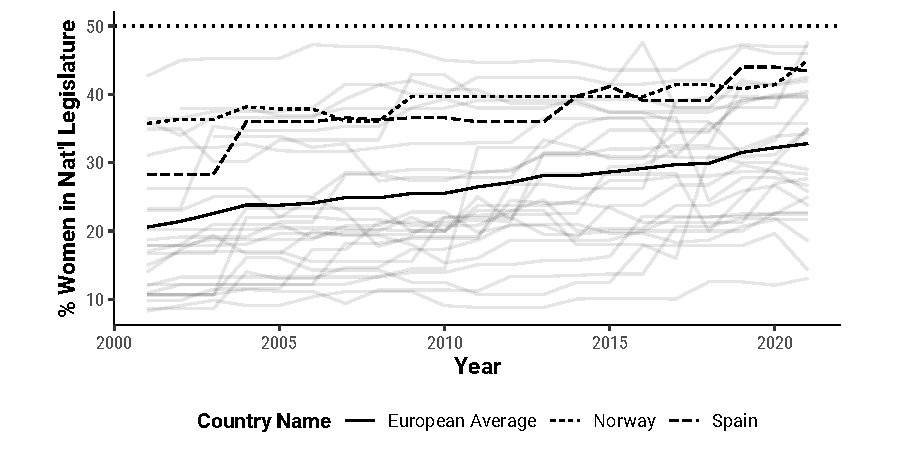
\includegraphics[width = 0.75\textwidth]{../output/figures/csts_plot.pdf}
    \caption{Share of female legislators in national legislatures (lower houses) across European democracies (World Bank, 2023).}
    \label{fig:csts_plot}
\end{figure}

Evaluating the gender gap in political careers under PR is thus important for improving representation and democratic legitimacy. If women, once elected, have shorter tenures in office or miss out on promotion to senior office, their representation might still carry less weight, as they wield less power and experience in legislative processes. Moreover, if women suffer from diminished effects of being elected on future career progression, this might also contribute to a greater gender gap in representation at higher levels of political office.

One key aspect that may drive the gender gap in political careers is whether there is a difference in the effect of being elected on running again and winning again as the most proximate candidate-levels outcomes of winning office. Any gender differential in the effect of being re-elected will have knock-on effects on future downstream career outcomes (such as running for or winning election to the national legislature). Studying this first outcome therefore sheds light on where the `leaky pipeline' begins, and is, so far, understudied for the domain of PR \citep{smrek2020}.

\subsection{When Does PR Create Similar Incumbency Advantages for Men and Women?}

How, if at all, should we expect incumbency advantages under PR to differ by candidates' gender? More candidate-centred (i.e., open-list) systems, in which voters can determine the ranking of individual candidates, may render women more vulnerable to voter and systemic biases, and lead to a smaller incumbency advantage compared to men.

Table \ref{tab:inc_mechanisms} summarizes the argument. The primary incumbency advantage mechanism in closed-list systems -- rank increases due to seniority -- is unlikely to produce a gender gap, even if party elites are unconditionally biased against women. By contrast, a key mechanism in open-list PR systems -- an increase in personal votes due to name recognition -- may be reduced for women and produce a smaller incumbency advantage for female candidates if voters are biased or update less on female incumbents due to systemic bias. Altogether, closed- and open-list PR systems have different mechanisms through which the incumbency advantage operates. This, in turn, affects the gender gap in incumbency advantages -- irrespective of any unconditional differences in how likely men or women are to win office. Below, I elaborate on the incumbency mechanisms and their vulnerability towards gender biases in each setting.

\begin{table}[thbp]
    \centering\begin{tabular}{lcc}
        \toprule
         & \textbf{Closed-list} & \textbf{Open-list} \\
        \cmidrule(lr){1-3}
        Incumbency Effect Mechanisms & & \\
        \, \emph{Party-driven} &  Seniority  & Seniority \\
        & Resource Advantage & Resource Advantage \\
        & (rank advance) & (pre-vote rank advance) \\[2mm]
        \, \emph{Voter-driven}  &                          & Name Recognition  \\
                  & & (pref vote increase) \\[2mm]
       Gender Gap Mechanisms & Social Learning (\textbf{+}) & Social Learning (\textbf{+}) \\
                   & & Voter Bias (\textbf{-}) \\
                   & & Systemic Bias (\textbf{-}) \\
    \bottomrule
    \end{tabular}
    \caption{Main Incumbency Advantage Mechanisms under Proportional Representation}
    \label{tab:inc_mechanisms}
\end{table}

\paragraph*{Closed-list PR.} In closed-list PR, the rank order of list positions decides individuals' electoral fortunes: higher list ranks translate into greater electoral security. Mechanically -- as long as voters' decision what party to vote for does not depend on the position of individual candidates -- any incumbency advantage for barely elected politicians must come from an improved list rank.\footnote{The larger the district magnitude, the easier this assumption becomes to satisfy. With dozens of candidates on a party list, voters are unlikely to switch their ballot to another party because of a single candidate that they dislike.} Put differently, candidates who are just barely elected move up to a safer list position with a higher chance of winning office in the next election. This mechanism is often institutionalized as a seniority norm in closed-list PR systems \citep[cf.][]{cirone2020}. Alternatively, even where no strong official seniority norm exists, incumbents (compared to non-incumbents) may be able to marshal significantly greater resources and stronger networks at their disposal in order to occupy any better ranked list positions when vacancies open up \citep{trounstine2010modern,nunez2018clientelistic}.

Note that party elites may treat male and female candidates quite differently in an unconditional sense: across the whole set of available list positions, they may, on average, rank women in lower positions; they may also assign female candidates to more (or less) competitive districts. There are two primary explanations for this phenomenon: one is that party elites are biased against female candidates themselves (which is discussed below); the other is that they engage in strategic ranking behavior in order to maximize the party's vote share. In practice, however, there is limited evidence that voters -- who cast votes for whole party lists, not individual candidates -- are highly sensitive to the gender composition of the party list \citep{bagues2020a}, especially in elections with high district magnitude.

However, when comparing incumbency advantages among barely elected winners -- that is, thinking about the additional effect \emph{conditional} on winning office -- we need to consider whether party elites' behavior shows any meaningful gender difference in response to getting elected. The question here is no longer whether women experience greater obstacles towards being elected overall, but whether, once they are elected (and in comparison to men in a similar position), they experience similar rank improvements and hence incumbency advantages of a similar magnitude as male candidates.

More specifically, consider two distinct scenarios regarding party elite bias, with different implications for the incumbency gender gap under closed-list PR. First, assume that party elites treat male and female candidates equally across the whole list; hence, both male and female barely elected winners are of the same quality. Quality can, for example, mean greater effectiveness as a policymaker, responsiveness to voters \citep{anzia2011}, or greater success in securing funding for the municipality. Why should the party leadership advance male winners faster towards safer list positions than female winners? One answer could be that parties decide candidate placement strategically in order attract voters who are biased towards or prefer male candidates. If such voters and punish lists with too many women at the top, parties may want to boost male incumbents further and award them more advantageous positions. However, as mentioned before, there is limited evidence party lists that increase the share of women on the list are being punished at the ballot box \citep{bagues2020a}.


Second, party leadership may still exhibit unconditional negative biases towards women -- for example, in the form of lower initial placements or a penalty to their perceived quality \citep{luhiste2015,murray2012,krook2014}. One corollary of this assumption is that female candidates in the sample of barely elected or barely losing candidates will likely be, on average, of higher quality than men in comparable positions \citep{ashworth2021,besley2017}.\footnote{This follows from women having to overcome the bias term in the first place in order to advance to the threshold position, similar to \citet{ashworth2021}.}

If a female candidate who overcomes the initial bias term (e.g. with high quality on the aforementioned dimensions such as lobbying more effectively on behalf of the municipality) and proceeds through the list ranks towards the set of barely elected candidates, it is hard to imagine why parties would further increase their negative bias of women as a result of being elected. Another reason why parties ought to be consistent in their treatment of barely elected candidates is strategic incentives: if the party were to deny women an incumbency advantage (of a similar magnitude as men's), they would be less likely to run and compete in the first place. Put differently, it would be counterproductive to recruit female candidates in the first place, put them in competitive list positions, only to deny them further advancement.

If anything, parties should reduce their negative stereotypes upon observing a female candidate in office perform well: their perception should move closer to the candidate's true ability. If this is the case, and the elites' initial perception was biased downward, women should actually experience a \emph{greater} incumbency advantage than men. Alternatively, female candidates who have overcome initial hurdles and succeeded into the set of list ranks around the election threshold may have greater access to resources and political connections than men of similar list rank -- which female winners may be able to turn into a differentially greater incumbency advantage. An important caveat to this argument is that women may suffer from lower persistence in political careers even after winning elections due to asymmetric outside factors (e.g., higher divorce rates, see \citet{folke2020}), or more general differences in persistence or motivation to run for office \citep{lawless2005, wasserman2020,ashworth2021}).

\paragraph*{Open-list PR.} In open-list (and more candidate-centred) PR systems, part of the incumbency advantage comes from voters awarding elected candidates a boost in preference votes, therefore making it more likely that they will be re-elected \citep{dahlgaard2016, dettman2017, jankowski2021}.\footnote{\citet{fiva2018a}, also studying Norwegian local elections, find the overall effect of incumbency on personal vote shares to be small and statistically indistinguishable from zero. This is likely the result of a particular operationalisation of personal vote share. I discuss this issue further in Appendix \ref{app:norway_pv_estimation} and show that my results -- demonstrating that there is a meaningful effect for male candidates -- hold up across different operationalisations.} In lower-level, low-information elections, such as municipal elections, voters rarely observe the quality of candidates precisely. Instead, they might follow established heuristics in the form of incumbency status, (pre-vote) list rank, and name recognition \citep{dettman2017}. Voters typically only have a limited number of preference votes (e.g. in Norway, one-quarter of the council size) that they can allocate across the party list.\footnote{If parties can still decide the order in which candidates appear on the ballot, they may still be able to affect candidates' success, which is strongly correlated with the initial list position (Appendix \ref{app:pv_by_rank}). In that sense, parties in open-list determine which candidates enter the set of \emph{viable} candidates, but do not have fully discrete power to decide who gets elected.}

In this context, women may experience a diminished incumbency advantage if a subset of voters awards their preference votes to incumbent men, but not women. Consider a pool of voters in which some voters allocate preference votes based on candidates' true quality (perhaps with a noisy, but unbiased signal), while others use name recognition and incumbency as a heuristic; a subset of these heuristic voters only awards preference votes to male incumbents.

Women may still be able to win initial election, carried forward by unbiased voters. However, barely elected men will experience a greater increase in preference votes than barely elected women thanks to male-favoring heuristic voters. (Appendix \ref{app:theorysim} illustrates this argument further with a toy model simulation). With a smaller increase in preference votes, women will also observe a smaller increase in their probability of winning again as an effect of barely winning.\footnote{As in the closed-list case, my theoretical argument does not make a claim about an unconditional difference in candidate type between male and female candidates. If women suffer from a `sticky floor', the entire threshold sample of female candidates may be of higher quality compared to the respective male one. Yet, any alternative explanation focussed on differential selection needs to explain why there is an additional effect for men (or women) coming into force as a result of being barely elected. One such potential alternative could be that, as in closed-list PR, high-quality women have access to more expansive political networks or resources which, once elected, becomes differentially more useful as an incumbent. This would attenuate any negative gender gap in incumbency advantages in open-list PR.}

There may be multiple, observationally equivalent, reasons why some voters do not award preference votes to female incumbents. One answer may be simple voter bias. A rich literature studying unconditional voter biases against women yields ambiguous results \citep{krook2014,krook2018,golder2017a,ragauskas2019}. Survey experiments and quasi-experimental evidence conducted in plurality settings suggest that unconditional voter biases against women exist, but may be context- and party-specific \citep{anzia2019,eymmoud2017, horiuchi2020,cipullo2021}. It is less costly for voters to act on their biases in an open-list PR system: they can vote for co-partisans and thus need not trade off ideological proximity with a preference for candidates of a certain sex \citep[cf. aversive sexism, ][]{batista2020electoral}. This stands in contrast to closed-list PR, where voters with a dislike for the gender composition of their preferred list only have the alternative of voting for another list, and will have to decide between ideological proximity and gender preference. Existing literature also focusses on voter biases preventing women from being elected in the first place; it remains an open question through what channels voter bias may affect typical incumbency mechanisms, and whether voters change their biases in response to women getting elected.\footnote{For example, male-preferring voters may increase their observable bias after the election of a woman as they update on the probability of a woman elected and/or societal preferences.}

If it is voter bias that drives this gender gap, then we should expect to see a more pronounced gap in right-wing parties where we think that voters in these parties are either more personally biased, or subject to greater systemic biases (e.g. read more biased newspapers). Another reason this could hold true is that men form the majority of right-wing voters, and and may prefer to vote for candidates of the same gender -- either because of their own bias towards similar candidates, or because they expect male candidates to be a closer match based on policy preferences and salience of represented issues (e.g. on social issues regarding gender equality).

Finally, systemic bias, rather than voter bias, may account for the gender differential in preference vote increases: if local media report less frequently or less positively about female incumbents, then they may attain smaller name recognition bonuses, and will accrue smaller preference vote boosts despite (heuristic) voters themselves being unbiased.

In sum, my argument leads to the following expectation for open-list PR: the differential increase in preference votes as an effect of winning is an incumbency advantage mechanism that is voter-driven, therefore only available in open-list PR, and will only kick in for incumbent men and women, but not for barely losing candidates. As a consequence, we should observe a smaller incumbency advantage for women compared to men.

% ----------------------------
% SECTION 3 -- DATA AND DESIGN
% ----------------------------

\section{Data and Design}

How can we study the gender gap in political careers, and incumbency advantages more specifically, under proportional representation? In this section, I describe my case selection, data sources, and research design.

\subsection{Cases and Data}

In an ideal world, my case selection would exploit within-country (and within-election) variation in electoral rules to mitigate the concern of unobserved cross-country differences. Unfortunately, no such straightforward setting exists that would allow for estimation with sufficient statistical power.\footnote{I do leverage variation in Norway's electoral rules across tiers of government later in the paper. However, the results from higher-order elections are noisy, as heterogeneity-in-discontinuity designs require a lot of data for sufficient power.} Instead, I turn to a comparison of local elections across countries. By studying local elections -- the typical entry point for political careers -- we can understand whether electoral systems can have repercussions for women's political careers that cascade into higher levels of office, and contribute to fewer and less experienced female candidates in more senior offices \citep{cirone2020}.

To estimate the gender gap in incumbency advantages, I use local elections between 2003 and 2019 in two countries -- Norway (open-list) and Spain (closed-list), along with supplementary data from Poland's open-list county elections.\footnote{In both cases, this is the widest range of elections for which data is available. Given the overall increasing trend in women's representation over time, including data from years prior will yield a diminishing contribution to improved statistical power; moreover, it is unclear if estimating the gender gap from more than two decades ago would yield informative results about today's career dynamics.}

In Norway's form of open-list PR, voters cast preferences for individual candidates \emph{within} a party, which ultimately determines list rankings and, consequently, which candidates are successful in winning a seat. Party elites do come up with an \emph{ex ante} ordering of candidates appearing on the ballot. They also award a `pre-advantage' status to a limited number of candidates that allocates them additional preference votes compared to non-advantaged candidates.\footnote{Each candidate with pre-advantage is awarded a bonus number of preference votes equal to 25\% of all votes cast for the party list.} These two features distinguish Norway's electoral system (and lead some to call it semi-open). Nonetheless, it is ultimately voters' allocation of preference votes that decides on the \emph{ex post} rank ordering.\footnote{Voters' preference votes have proved decisive in electing about 25\% of candidates -- see footnote 3.} Norway's municipal elections are set on a fixed four-year cycle and determine the composition of the municipal council, which then elects the mayor. The competition in these elections is organised along the lines of the national party system, with a 'left' and a 'right' block. Overall, there are 356 municipalities in Norway, which form the lowest rung of the country's administrative structure. Although there is no legally binding gender quota in Norway's municipal elections, some parties on the left have imposed a voluntary one. However, these quotas only enforce the overall number of women on the list, whereas their ultimate ranking is still up to the voter's preference votes. For this reason, these quotas are unlikely to exert much `bite' in the context of the close loser/winner threshold sample.

By contrast, Spain's elections at the most local level of politics use closed-list PR. Voters can only cast their ballot for fixed lists of candidates put forward by political parties; the order of list rankings on the ballot is ex ante determined by the local party leadership. These elections are also held on a fixed four-year cycle (that coincides with Norway's, meaning that local elections are held in the same year in each country), and are also dominated by lists representing the dominant national parties -- especially PP and PSOE, who retain the institutional strength and depth to contest the vast majority of these elections. Since 2007, municipalities over the threshold of 3,000 population (5,000 between 2003 and 2007) have a legally binding quota that requires party lists to field at least 40\% candidates (although the quota is silent on where they are placed).\footnote{Appendix \ref{app:below_quota} shows that my results are unlikely to be driven by the quota rule.} There are slightly over 8,000 municipalities in Spain; those with fewer than 250 inhabitants use a different electoral system (block voting) and are excluded from the analysis below. Above the municipality, there are two additional layers of regional government (provinces, autonomous communities).

Apart from the different electoral system, the two cases share many similarities. Both countries feature indirectly elected municipal executives at the local level and hold elections in a regular, fixed four-year cycle. Importantly, both countries also rank highly in terms of their overall share of women's representation in the national legislature, as well as in lower-ranked levels of government.\footnote{In the analysis sample of bare losers and bare winners, 38\% of candidates in Norwegian local elections and 35\% in Spanish local elections are women. See also Figure \ref{fig:csts_plot}} They also rank below average in terms of societal biases against women: The UN Gender Social Norms Index reports that about 20\% of respondents in Norway showed a negative bias towards women in politics; the proportion was close to 30\% in Spain.
Despite great care to account for differences between the two cases, and additional analyses consistent with the argument, it is important to stress that the cross-country comparison nonetheless remains suggestive: we still require more work to credibly estimate the true effect of different shades of PR on the gender gap in political careers.

I collect my data for this analysis from two main sources. Data on elections and candidates in Norway come from \citet{fiva2020}, who helpfully already code unique candidate identifiers across multiple election cycles. I drop all candidates that the original authors flagged as inconsistent, as well as those from minor or non-partisan lists.\footnote{The data source flags around 30\% of observations in the threshold sample as belonging to municipalities where non-threshold candidates' preference vote records may be missing (usually from minor parties). However, all of the candidates in the threshold sample itself feature fully recorded preference votes, list rank and election outcomes. Including flagged municipalities is therefore unlikely to affect data quality in the threshold sample itself. Appendix \ref{app:norway_restricted} reports results from a more restricted sample and finds no meaningful difference in the results.} Data on elections and candidates in Spain come from the country's Ministry of Interior (\texttt{http://www.infoelectoral.mir.es}). To link candidate records across time, I converted candidate names to lower case, substituted common abbreviations and linked records if the Jaro-Winkler distance between two full names in the same municipality was less than 0.1.\footnote{The Jaro-Winkler distance measures the edit distance between two strings: a lower score implies fewer edits are necessary to move from one string to another.} Because the original data do not report candidates' gender before 2007, I classified their gender in 2003 based on the probability that the same first name was assigned as either male or female in subsequent elections.\footnote{I fit a linear regression model predicting gender on post-2003 observations' first name, and use the fitted model to predict first names' gender in 2003. I drop observations whose first name only appears in 2003.}

In both cases, I drop observations from cities with a population above 250,000 to ensure that locations with unusually high district magnitude and, in some cases, additional institutional powers, do not drive my results.\footnote{For example, the municipality of Oslo merges two layers of government (municipal and regional) into one. Some of Spain's largest municipalities such as Madrid or Barcelona, also feature exceptionally high-profile local politics with national coverage, far larger budgets and greater policy-making powers. There are two municipalities in Norway and six in Spain that are above the chosen population threshold. My results do not change meaningfully when retaining them in the data.} Moreover, in order to maintain the as-if random assumption around the threshold, I follow \citet{fiva2018a} and restrict my sample to candidates whose list rank meant that they were the last one within their party to win a seat or the first ones to be defeated.

\subsection{Empirical Strategy}

\subsubsection{Defining the Gender Gap in the Incumbency Advantage}

I first discuss the estimand of interest before introducing the estimator and empirical design. Put simply, in each country, I am interested in the gender gap (the difference between men and women) in the effect of being elected (the `incumbency effect') on the candidate's future electoral trajectory -- whether they run again and whether they are re-elected. This \emph{difference} between two causal estimates, which I call the gender gap in the incumbency advantage, is formally defined as follows (using potential outcomes notation):

\begin{equation}
\tau_F - \tau_M = (E[Y_{1i} | s_i = F] - E[Y_{0i} | s_i = F]) - (E[Y_{1i} | s_i = M] - E[Y_{0i} | s_i = M])
\end{equation}

where $Y$ denotes the (potential) outcome of interest, and $s_i$ is the candidate's gender.
This set-up is closely related to estimating the moderation effect of gender on the incumbency effect, although the difference in heterogeneous effects subsumes both the causal effect of gender and that of correlated attributes \citep{bansak2021}.\footnote{
    Throughout this paper, I estimate the incumbency effect with respect to gender as a 'bundle' of characteristics \citep[cf.][]{sen2016}. This is different from estimating the effect of a female candidate counterfactually running as a man (but with all other characteristics kept constant otherwise \citep{marshall2021}).
}

My key outcomes after the first election are whether the candidate \emph{runs again} in the next election, and whether they \emph{win} in the next election. Following \citet{demagalhaes2015}, I am interested in the unconditional effect of winning in $t$ on election in $t+1$ -- that is, if a candidate does not run again in $t + 1$, they are coded as a `0' on re-election.\footnote{Conditioning on running again in the future runs the risk of introducing post-treatment bias. See also \citet{hyytinen2018a,cirone2020}.} I focus on the next election outcome as my primary interest, because it is the immediate next step in politicians' careers. If a gender gap already exists at this stage, it will proliferate into future outcomes such as running (or winning) in $t + 2$ or running (or winning) in higher-order elections. Estimating the gender gap at the first stepping stone therefore provides the most direct measurement of the level of gender inequity.

\subsubsection{Estimating the Gender Gap Using A Heterogeneity-in-Discontinuity Design}

How can we estimate the theoretical quantity of interest? A typical regression discontinuity (RD) design, widely applied in the study of incumbency effects \citep[e.g.][]{lee2001a,demagalhaes2015,folke2016d}, compares candidates who have just missed out on being elected by a few votes to those who have just crossed the threshold and found themselves elected. The design recovers the local average treatment effect of being elected. It retains its causal interpretation when restricted to a comparison within a subgroup, in which case the RD design recovers the subgroup-specific local average treatment effect.

While the incumbency effect \emph{within} each gender can be causally identified using a regression discontinuity between bare winners and bare losers, the \emph{difference} between the two conditional effects is not causally identified \citep{wasserman2020,brown2019}. Male and female candidates around the election threshold may differ from one another on a number of observable as well as unobservable characteristics. In that sense, the main objective of the paper, consistent with the previously defined estimand, is to estimate whether there is heterogeneity in the magnitude of the incumbency effect based on candidates' gender (and the bundle of differences associated with it).

To study the heterogeneity in the incumbency effect between male and female candidates, I estimate the following heterogeneity-in-discontinuity specification:

\begin{align}
\begin{split}
    y_{it} & = f(MV_{it}) + \beta_1 D_{it} + \beta_2 F_{it} + f(MV_{it}, D_{it}) + f(MV_{it}, F_{it}) +  \\
    &  \ \beta_3 (D_{it} \times F_{it}) + f(D_{it}, F_{it}, MV_{it}) + \theta_{i} + \phi_{it} + \epsilon_{it}
\end{split}
\end{align}

\noindent where $MV$ denotes the margin of victory (the running variable), $D$ is a dummy for whether the candidate is elected or not, and $F$ is a dummy for whether the candidate is female. $i$ is a subscript for the individual candidate running in an election at time $t$. In this setup, $\hat{\beta_1}$ recovers the incumbency effect for males, and $\hat{\beta_3}$ recovers the gender gap in the incumbency effect.
I also include county or province ($\theta_i$) and year-by-party fixed effects ($\phi_{it}$). Unless noted otherwise, I report robust standard errors clustered by municipality.

Throughout the paper, I present estimates using local linear regression with first-order polynomials \citep[cf.][]{gelman2018} and a uniform kernel.\footnote{My results remain robust to dropping fixed effects or using other common (e.g., triangular) kernels (cf. Appendices \ref{app:kernelchoice} and \ref{app:nofe}).} Because the estimation of the treatment effect in either group depends on the functional form of the conditional expectation function modelling the outcome at the threshold, my estimates might be biased if my functional form $f(MV)$ is misspecified. I therefore also report results using a second-order polynomial specification in Appendix \ref{app:rd_polynomial}. Finally, the estimates from regression discontinuity may be sensitive to the chosen bandwidth around the threshold. To compute the optimal bandwidth on which I fit my specification, I use Calonico, Cattaneo and Titiunik's (\citeyear{calonico2014}) approach when run on the full sample (including both men and women).\footnote{I follow \citet{cipullo2021} in this approach.} Again, to show robustness across modelling choices, I also present estimates when the bandwidth is set to one-half and twice the optimal width in the main tables, and show robustness to further bandwidth choices in Appendix \ref{app:bandwidth_sensitivity}.

As with every RD-based design, my identification assumptions may be confounded if candidates have the ability to sort themselves around the threshold, or if parties can anticipate the election result with high accuracy, thus successfully predicting which list ranks will be elected. I report the typical robustness checks (continuity in density around the threshold and covariate balance) in Appendices \ref{app:density_checks} and  \ref{app:density_covariates}.

\subsubsection{Identifying Bare Winners And Bare Losers In Proportional Representation}

In the context of PR elections, constructing the running variable and identifying which candidates came close to barely losing or barely winning is not as straightforward as in the archetypal plurality case \citep{lee2001a,lee2008, fiva2016,fiva2018b}. To do so, I use and extend methods developed and applied by \citet{folke2014} and \citet{fiva2018a} in the context of closed-list and open-list PR elections, respectively. I describe both of these methods in greater detail in Appendix \ref{app:pr_running}.

% --------------------------
% SECTION 4 -- MAIN RESULTS
% --------------------------

\section{Main Results: Negative Gender Gap In Open-List, But Not Closed-List PR}

\begin{figure}[htbp]
    \centering
    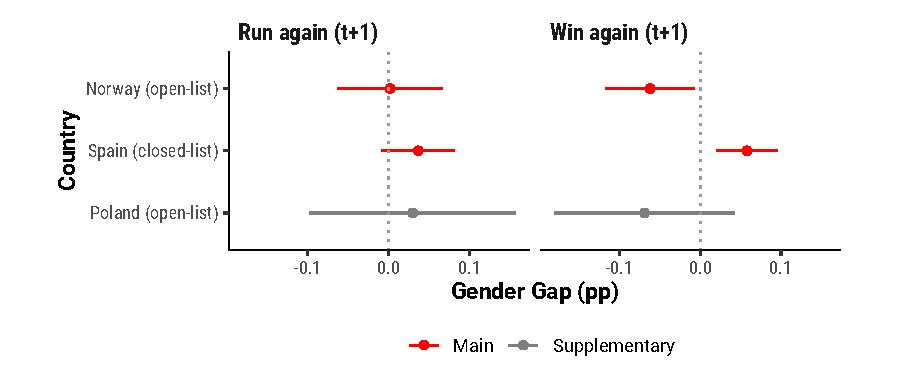
\includegraphics[width = 0.8\textwidth]{../output/figures/coef_summary.pdf}
    \caption{\textbf{Estimated Gender Gap in Incumbency Advantages Across Cases.} Point estimates from preferred heterogeneity-in-discontinuity specifications, with 95\% Confidence Intervals.}
    \label{fig:coef_summary}
\end{figure}


Figure \ref{fig:coef_summary} plots the difference in estimated incumbency effects between men and women for local elections in Norway (open-list) and Spain (closed-list), along with noisier, supplementary, estimates from Polish county-level elections (open-list).
There is no statistically significant gender gap in the effect of winning on running again in any country.
There is, however, a pronounced contrast in the effect on winning again: in Norway, women suffer from a far smaller incumbency advantage than their male colleagues (by about 7 pp), whereas female candidates in Spain experience a differentially larger incumbency advantage than men (by about 6 pp). Both estimates are statistically significant at conventional levels.
The gender gap under open-list PR likely replicates to similar settings outside Norway, as the results for Poland suggest (see Appendix \ref{app:poland}).

\begin{figure}[!htb]
    \centering
    \begin{subfigure}[t]{0.98\textwidth}
        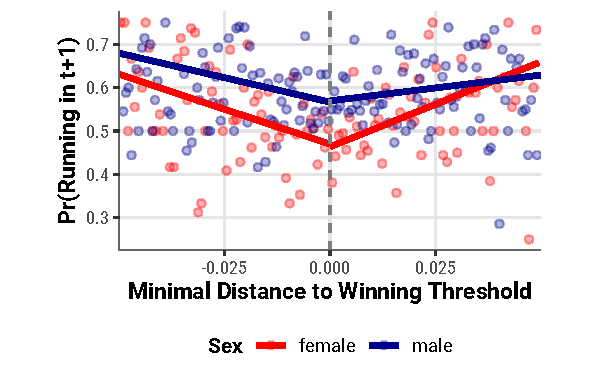
\includegraphics[width = 0.48\textwidth]{../output/figures/norway_run_again.pdf}
        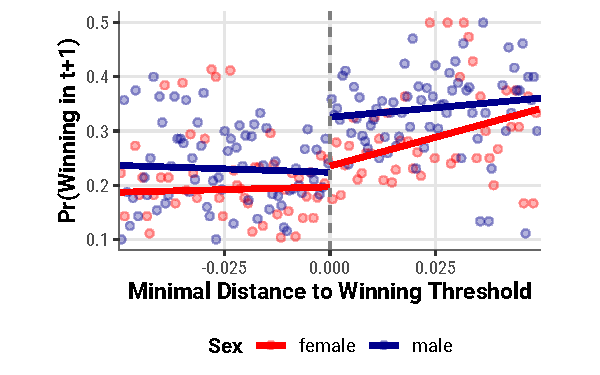
\includegraphics[width = 0.48\textwidth]{../output/figures/norway_win_again.pdf}
        \caption{Norwegian Local Elections \label{fig:main_plot_norway}}
    \end{subfigure}
    \begin{subfigure}[t]{0.98\textwidth}
        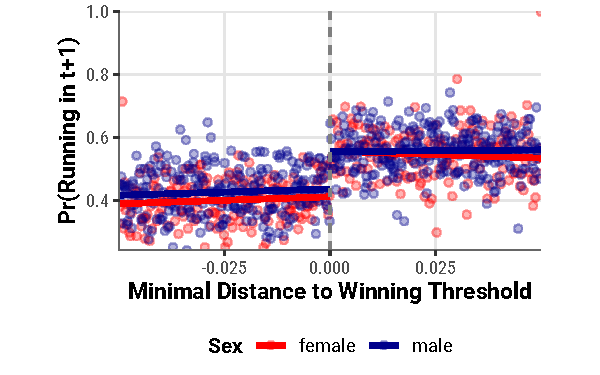
\includegraphics[width = 0.48\textwidth]{../output/figures/spain_run_again.pdf}
        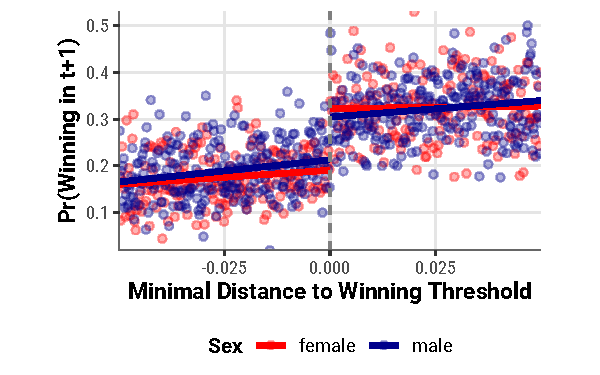
\includegraphics[width = 0.48\textwidth]{../output/figures/spain_win_again.pdf}
        \caption{Spanish Local Elections \label{fig:main_plot_spain}}
    \end{subfigure}
    \caption{\textbf{Effect of Winning Election on Running Again and Winning Again, By Gender And Case.} The visual regression discontinuities compare bare winners and bare losers by candidates' gender.}
    \label{fig:main_plot}
\end{figure}


Figure \ref{fig:main_plot} presents these findings in a graphical representation of the difference in discontinuities. Panel (a) shows the data from Norwegian open-list elections. Women, while unconditionally less likely to run again (left panel), do not suffer from any additional disadvantage in \emph{running again} compared to men once elected:
losing an election does not diminish women's persistence differentially. While barely winning increases the probability of \emph{winning again} for candidates of either gender (right panel), the effect is clearly greater for male candidates (4 percentage points for women vs. 10 percentage points for men). This matches the results from Figure \ref{fig:coef_summary}. Turning to Spanish closed-list elections in (b), we similarly observe no gender difference in the effect of winning on running again; candidates of either gender experience an increase of approximately 9 percentage points in the probability of winning again as a result of getting elected. Unlike in the Norwegian case, the Figure does not show a visually obvious gender gap; if anything, the effect appears somewhat larger for women.

In the remainder of this section, I parse these headline results in greater detail and provide additional results to guard against likely alternative explanations.

\subsection{Norway (Open-List PR)}

Turning to Norway's open-list elections first, Table \ref{tab:norway_main} backs up the graphical intuition with formal evidence in the form of heterogeneity-in-discontinuity estimates. Columns 1 to 3 report estimates of the effect of winning on running again in $t + 1$. Both the effect of being elected, as well as the gender gap coefficient, are close to zero across all bandwidth choices.

\begin{table}

\caption{\label{tab:norway_main} \textbf{Difference-in-Discontinuity Estimates For Incumbency Advantage In Norwegian Municipalities.} Women face diminished incumbency effect on winning again.}
\centering
\fontsize{9}{11}\selectfont
\begin{threeparttable}
\begin{tabular}[t]{lS[
              input-symbols=(),
              table-format=-1.3,
              table-space-text-pre    = (,
              table-space-text-post   = ),
              input-open-uncertainty  =,
              input-close-uncertainty = ,
              table-align-text-post = false]S[
              input-symbols=(),
              table-format=-1.3,
              table-space-text-pre    = (,
              table-space-text-post   = ),
              input-open-uncertainty  =,
              input-close-uncertainty = ,
              table-align-text-post = false]S[
              input-symbols=(),
              table-format=-1.3,
              table-space-text-pre    = (,
              table-space-text-post   = ),
              input-open-uncertainty  =,
              input-close-uncertainty = ,
              table-align-text-post = false]S[
              input-symbols=(),
              table-format=-1.3,
              table-space-text-pre    = (,
              table-space-text-post   = ),
              input-open-uncertainty  =,
              input-close-uncertainty = ,
              table-align-text-post = false]S[
              input-symbols=(),
              table-format=-1.3,
              table-space-text-pre    = (,
              table-space-text-post   = ),
              input-open-uncertainty  =,
              input-close-uncertainty = ,
              table-align-text-post = false]S[
              input-symbols=(),
              table-format=-1.3,
              table-space-text-pre    = (,
              table-space-text-post   = ),
              input-open-uncertainty  =,
              input-close-uncertainty = ,
              table-align-text-post = false]}
\toprule
\multicolumn{1}{c}{ } & \multicolumn{3}{c}{Run (t + 1)} & \multicolumn{3}{c}{Win (t + 1)} \\
\cmidrule(l{3pt}r{3pt}){2-4} \cmidrule(l{3pt}r{3pt}){5-7}
  & \multicolumn{1}{c}{(1)} & \multicolumn{1}{c}{(2)} & \multicolumn{1}{c}{(3)} & \multicolumn{1}{c}{(4)} & \multicolumn{1}{c}{(5)} & \multicolumn{1}{c}{(6)}\\
\midrule
Elected & 0.002 & -0.010 & 0.016 & 0.107 & 0.102 & 0.109\\
 & (0.019) & (0.016) & (0.024) & (0.017) & (0.015) & (0.021)\\
\addlinespace
Female & -0.097 & -0.092 & -0.085 & -0.027 & -0.024 & -0.026\\
 & (0.021) & (0.018) & (0.026) & (0.018) & (0.015) & (0.021)\\
\addlinespace
Elected x Female & 0.002 & 0.024 & -0.030 & -0.062 & -0.047 & -0.096\\
 & (0.033) & (0.028) & (0.039) & (0.028) & (0.024) & (0.034)\\
\addlinespace \midrule \addlinespace
Bandwidth & 0.054 & 0.11 & 0.027 & 0.05 & 0.099 & 0.025\\
BW Type & \multicolumn{1}{c}{Optimal} & \multicolumn{1}{c}{2x Opt} & \multicolumn{1}{c}{0.5x Opt} & \multicolumn{1}{c}{Optimal} & \multicolumn{1}{c}{2x Opt} & \multicolumn{1}{c}{0.5x Opt}\\
Outcome Mean & 0.564 & 0.575 & 0.551 & 0.261 & 0.263 & 0.257\\
N (left) & \multicolumn{1}{c}{4617} & \multicolumn{1}{c}{5529} & \multicolumn{1}{c}{3667} & \multicolumn{1}{c}{4502} & \multicolumn{1}{c}{5428} & \multicolumn{1}{c}{3549}\\
N (right) & \multicolumn{1}{c}{4666} & \multicolumn{1}{c}{5590} & \multicolumn{1}{c}{3711} & \multicolumn{1}{c}{4551} & \multicolumn{1}{c}{5489} & \multicolumn{1}{c}{3592}\\
\bottomrule
\end{tabular}
\begin{tablenotes}[para]
\item All estimates are reported with robust standard errors clustered at the municipality level in parentheses. Each observation is a candidate's election attempt. 'Elected' is an indicator for observations where the candidate obtained a seat in the municipal council. 'Female' is an indicator for observations identified as female. `Elected` times `Female` is the interaction between the two variables. Other coefficients (running variable) reported in Table I1. Regression run on all candidates in elections between 2003 and 2015. 
\end{tablenotes}
\end{threeparttable}
\end{table}

Columns 3 to 6 report the effect of winning on the probability of winning again in $t + 1$. For men, there is an increase of about 10 pp., which is statistically significant at all conventional levels. The interaction coefficient suggests that the incumbency advantage for women is approximately 6 pp. lower, which corresponds to a 60\% decrease in the magnitude of the effect. Although the precise magnitude of the difference between men and women varies between 5 and 10 pp. depending on the bandwidth, all interaction estimates are statistically significant.\footnote{For further robustness checks, Appendix \ref{app:bandwidth_sensitivity} reports the coefficients for a wide range of bandwidths. The results are also robust to dropping all municipalities in which some personal votes for candidates outside the threshold sample are recorded as missing (Appendix \ref{app:norway_restricted}), as well as to dropping outlying cities with very high populations (Appendix \ref{app:norway_outliers}).}

Together, these results constitute first evidence that female candidates in an open-list setting may suffer from a diminished incumbency advantage.

\subsection{Spain (Closed-List PR)}

I now turn to the results from closed-list elections in Spanish municipalities.

The formal estimates in Table \ref{tab:spain_main} corroborate the visual inspection and offer more precise results.
Once again, columns 1 to 3 report the effect of winning on running again in the next election.
There is a large and significant effect of winning on running again for men -- an approximately 10 percentage point increase, in line with the result from Figure \ref{fig:main_plot_spain}.
In this case, the gender gap is close to zero and statistically insignificant:
the effect of winning an election on running again appears to be of a very similar (or slightly larger in the case of some bandwidths) magnitude for women.

\begin{table}

\caption{\label{tab:spain_main} \textbf{Difference-in-Discontinuity Estimates For Incumbency Advantage In Spanish Municipalities}. Women likely enjoy a larger effect of winning on their probability to win again.}
\centering
\fontsize{9}{11}\selectfont
\begin{threeparttable}
\begin{tabular}[t]{lS[
              input-symbols=(),
              table-format=-1.3,
              table-space-text-pre    = (,
              table-space-text-post   = ),
              input-open-uncertainty  =,
              input-close-uncertainty = ,
              table-align-text-post = false]S[
              input-symbols=(),
              table-format=-1.3,
              table-space-text-pre    = (,
              table-space-text-post   = ),
              input-open-uncertainty  =,
              input-close-uncertainty = ,
              table-align-text-post = false]S[
              input-symbols=(),
              table-format=-1.3,
              table-space-text-pre    = (,
              table-space-text-post   = ),
              input-open-uncertainty  =,
              input-close-uncertainty = ,
              table-align-text-post = false]S[
              input-symbols=(),
              table-format=-1.3,
              table-space-text-pre    = (,
              table-space-text-post   = ),
              input-open-uncertainty  =,
              input-close-uncertainty = ,
              table-align-text-post = false]S[
              input-symbols=(),
              table-format=-1.3,
              table-space-text-pre    = (,
              table-space-text-post   = ),
              input-open-uncertainty  =,
              input-close-uncertainty = ,
              table-align-text-post = false]S[
              input-symbols=(),
              table-format=-1.3,
              table-space-text-pre    = (,
              table-space-text-post   = ),
              input-open-uncertainty  =,
              input-close-uncertainty = ,
              table-align-text-post = false]}
\toprule
\multicolumn{1}{c}{ } & \multicolumn{3}{c}{Run (t + 1)} & \multicolumn{3}{c}{Win (t + 1)} \\
\cmidrule(l{3pt}r{3pt}){2-4} \cmidrule(l{3pt}r{3pt}){5-7}
  & \multicolumn{1}{c}{(1)} & \multicolumn{1}{c}{(2)} & \multicolumn{1}{c}{(3)} & \multicolumn{1}{c}{(4)} & \multicolumn{1}{c}{(5)} & \multicolumn{1}{c}{(6)}\\
\midrule
Elected & 0.109 & 0.119 & 0.100 & 0.072 & 0.095 & 0.076\\
 & (0.014) & (0.010) & (0.020) & (0.012) & (0.008) & (0.017)\\
\addlinespace
Female & -0.024 & -0.032 & -0.012 & -0.032 & -0.026 & -0.033\\
 & (0.016) & (0.012) & (0.022) & (0.013) & (0.009) & (0.018)\\
\addlinespace
Elected x Female & 0.037 & 0.033 & 0.018 & 0.058 & 0.045 & 0.057\\
 & (0.023) & (0.017) & (0.032) & (0.019) & (0.013) & (0.027)\\
\addlinespace \midrule \addlinespace
Bandwidth & 0.032 & 0.064 & 0.016 & 0.035 & 0.071 & 0.018\\
BW Type & \multicolumn{1}{c}{Optimal} & \multicolumn{1}{c}{2x Opt} & \multicolumn{1}{c}{0.5x Opt} & \multicolumn{1}{c}{Optimal} & \multicolumn{1}{c}{2x Opt} & \multicolumn{1}{c}{0.5x Opt}\\
Outcome Mean & 0.486 & 0.483 & 0.485 & 0.256 & 0.251 & 0.254\\
N (left) & \multicolumn{1}{c}{14840} & \multicolumn{1}{c}{26294} & \multicolumn{1}{c}{7984} & \multicolumn{1}{c}{16223} & \multicolumn{1}{c}{28426} & \multicolumn{1}{c}{8726}\\
N (right) & \multicolumn{1}{c}{14729} & \multicolumn{1}{c}{26886} & \multicolumn{1}{c}{7825} & \multicolumn{1}{c}{16159} & \multicolumn{1}{c}{29072} & \multicolumn{1}{c}{8530}\\
\bottomrule
\end{tabular}
\begin{tablenotes}[para]
\item All estimates are reported with robust standard errors clustered at the municipality level in parentheses. Other coefficients (running variable) reported in Table I2. See Table 2 for additional details.
\end{tablenotes}
\end{threeparttable}
\end{table}

Columns 4 to 6 provide clear evidence that the incumbency effect on winning again is at least as great, if not bigger, for women.
Men experience an incumbency effect of an approximately 7 percentage point increase in their probability of winning the next election.\footnote{See Appendix \ref{app:rd_polynomial} for robustness to polynomial order, and Appendix \ref{app:bandwidth_sensitivity} for robustness to bandwidth choice. I also leverage the large number of observations in order to estimate a diff-in-diff sufficiently close to the threshold (within 1 percentage point) in Appendix \ref{app:spain_did}. The estimates are consistent with the results from Table~\ref{tab:spain_main}, and further point towards no large gender gap in the effect of winning on running again.} The gender gap coefficient is positive, and statistically significant at the optimal bandwidth (though not at other values), suggesting that the incumbency advantage is an additional 5 to 6 percentage points larger for women. This set of results suggests that women in Spanish local elections enjoy a somewhat \emph{greater} incumbency advantage than their male colleagues -- much in contrast to the findings in Norway's open-list PR setting.\footnote{In Appendix \ref{app:spain_by_party}, I check for any meaningful differences if I estimate the heterogeneity-in-discontinuity separately for either of Spain's two major parties. Second, in Appendix \ref{app:spain_by_quota}, I evaluate whether the results are meaningfully different for municipalities above that implemented a legally binding gender quota -- mandating that at least 40\% of all candidates be women -- versus those that did not. I do not find evidence of a negative gender gap for women across either type of municipality. In Appendix \ref{app:hetero_spain}, I also find no meaningful evidence that estimates differ by cities' population size, although the positive gender gap may be attenuated towards zero in cities in the highest population tercile.}

All told, the direct comparison between the results from Norway's open-list and Spain's closed-list elections is consistent with the theoretical argument that women suffer from disadvantages in incumbency effects where voters can determine individual candidates' list rankings. Still, on its own, this comparison cannot rule out that fundamental differences between Norway and Spain drive the set of results.

\subsection{Countries' Idiosyncracies Unlikely To Drive Gender Gap Difference}

Is the contrast in gender gap estimates the result of countries' idiosyncratic characteristics, rather than the product of electoral rules?

In Appendix \ref{app:case_extension}, I compare the gender gap in incumbency advantages across different electoral systems within the same country (Norway), and use the case of Poland's open-list local elections to demonstrate that the negative gender gap is not just an artefact of Norway's local politics.

Overall, the finding of a gender gap in incumbency advantages replicates for the same electoral system across different countries, but not for different electoral systems within the same country. This weakens (but cannot fully rule out) concerns about case selection driving the results and is consistent with the claim that differences in the type of proportional representation may affect the gender gap in political careers.

\subsection{Differential Selection Of Candidates Into Sample Unlikely To Drive Gender Gap}
\label{sec:diffsec}

In addition to concerns about the cross-country comparison discussed just above, we may also worry about threats to inference within any one case: if candidates' gender is also correlated with other characteristics, Norway's open-list results may simply reflect parties' or voters' preferences for the associated attribute, rather than gender itself \citep{bansak2021,teele2018}. Alternatively, female candidates in the threshold sample may run in different electoral environments (e.g. parties or geographies) that lead to smaller incumbency advantages \citep{folke2016a}. In both of these cases, differential selection into the sample could threaten the inference drawn from the observed gender gap.

I present two checks to guard against this explanation. First, I substitute gender with age and experience as conditioning variables in the difference-in-discontinuities setup in the Norwegian case.\footnote{Unfortunately, this is not possible to replicate in the Spanish case due to a lack of available candidate covariates.} My results in Appendix \ref{app:age_rd} suggest that there is no difference in the magnitude of the incumbency advantage between older and younger, or more and less experienced candidates.

Second, using a matching approach discussed in \citet{bansak2021} and \citet{bansak2022}, I compare female candidates to male candidates who are most similar on a number of individual- and election-level attributes. In Appendix \ref{app:matching}, I present results from various matched comparisons that remain consistent with my main findings.

Jointly, these results offer suggestive evidence that gender itself, rather than a correlated attribute, is a major factor driving the observed gender gap in incumbency advantages -- even though caveats about the finite nature of available covariates remain.

% -----------------------
% SECTION 5 - MECHANISMS
% -----------------------

\section{Mechanisms Behind the Gender Gap in Open-List PR}

What mechanism accounts for the stark difference in gender-specific incumbency advantages under open-list PR in Norway? In this section, I show that the gender gap is most pronounced among candidates in right-wing parties. I also find that voters in right-wing parties award a smaller increase in preference votes to female candidates as a result of being barely elected. This channel, mechanically unavailable in closed-list PR, is likely to contribute to women's smaller incumbency advantage in open-list settings. Put differently, this section provides suggestive evidence that the more candidate-centric nature of open-list PR opens the door to voter or systemic biases disproportionately affecting female candidates.

\subsection{Women's Disadvantage Concentrated in Right-Wing Parties}

\begin{table}[!h]

\caption{\label{tab:norway_by_party_inc} \textbf{Difference-in-Discontinuity Estimates For Incumbency Advantage In Norwegian Municipalities, By Political Party Group.}}
\centering
\fontsize{9}{11}\selectfont
\begin{threeparttable}
\begin{tabular}[t]{lS[
              input-symbols=(),
              table-format=-2.3,
              table-space-text-pre    = (,
              table-space-text-post   = ),
              input-open-uncertainty  =,
              input-close-uncertainty = ,
              table-align-text-post = false]S[
              input-symbols=(),
              table-format=-2.3,
              table-space-text-pre    = (,
              table-space-text-post   = ),
              input-open-uncertainty  =,
              input-close-uncertainty = ,
              table-align-text-post = false]S[
              input-symbols=(),
              table-format=-2.3,
              table-space-text-pre    = (,
              table-space-text-post   = ),
              input-open-uncertainty  =,
              input-close-uncertainty = ,
              table-align-text-post = false]S[
              input-symbols=(),
              table-format=-2.3,
              table-space-text-pre    = (,
              table-space-text-post   = ),
              input-open-uncertainty  =,
              input-close-uncertainty = ,
              table-align-text-post = false]}
\toprule
\multicolumn{1}{c}{ } & \multicolumn{2}{c}{Run (t+1)} & \multicolumn{2}{c}{Win (t+1)} \\
\cmidrule(l{3pt}r{3pt}){2-3} \cmidrule(l{3pt}r{3pt}){4-5}
  & \multicolumn{1}{c}{(1)} & \multicolumn{1}{c}{(2)} & \multicolumn{1}{c}{(3)} & \multicolumn{1}{c}{(4)}\\
\midrule
Elected & 0.022 & 0.005 & 0.086 & 0.126\\
 & (0.031) & (0.026) & (0.027) & (0.024)\\
\addlinespace
Female & -0.079 & -0.044 & -0.015 & -0.001\\
 & (0.034) & (0.030) & (0.027) & (0.025)\\
\addlinespace
Elected x Female & -0.040 & -0.014 & -0.053 & -0.089\\
 & (0.049) & (0.045) & (0.039) & (0.039)\\
\addlinespace \midrule \addlinespace
Parties & \multicolumn{1}{c}{Left} & \multicolumn{1}{c}{Right} & \multicolumn{1}{c}{Left} & \multicolumn{1}{c}{Right}\\
Bandwidth & 0.05 & 0.068 & 0.052 & 0.069\\
Outcome Mean & 0.546 & 0.59 & 0.253 & 0.26\\
N (left) & \multicolumn{1}{c}{1568} & \multicolumn{1}{c}{2382} & \multicolumn{1}{c}{1580} & \multicolumn{1}{c}{2388}\\
N (right) & \multicolumn{1}{c}{1589} & \multicolumn{1}{c}{2413} & \multicolumn{1}{c}{1601} & \multicolumn{1}{c}{2419}\\
\bottomrule
\end{tabular}
\begin{tablenotes}[para]
\item All estimates are reported with robust standard errors clustered at the municipality level in parentheses. Each observation is a candidate's election attempt. Other coefficients reported in Table I3.
\end{tablenotes}
\end{threeparttable}
\end{table}

Is the gender gap in the incumbency advantage persistent across parties from the entire spectrum of political ideologies? Both parties and voters following a more socially conservative ideology might be more inclined to exhibit a negative bias towards women, thus diminishing their incumbency advantage.\footnote{Appendix \ref{app:spain_by_party} repeats the same procedure for the Spanish case. } Although merely suggestive, a stark contrast between party families may also point towards voter bias, rather than universal, systemic bias, as a key mechanism.

I estimate the heterogeneity-in-discontinuity separately on subsamples of candidates from left-leaning and right-leaning parties and report the results in Table \ref{tab:norway_by_party_inc}.\footnote{Parties classified as 'left' are Labour and the Socialist Left. Parties classified as `right' are the Conservatives, (the right-wing populist) Progress, the Christian Democratic Party, and the Liberal Party, corresponding to the two 'coalition blocs' in Norwegian politics. I exclude the Centre Party, which has joined both left-wing and right-wing coalitions in recent decades.}  Columns 1 and 2 report the effect of winning on running again by subsample. Although noisier than the main results, we see the same finding replicated as in Table \ref{tab:norway_main}. There is no meaningful effect of being elected on running again in the next election for male candidates; nor is there a statistically significant difference in the effect between genders.

Columns 3 and 4 report the effect of winning on whether the candidate is elected in the next election. In left-wing parties, both the absolute incumbency effect for men, as well as the magnitude of the gender gap are smaller. Though the point estimate still suggests a 5 pp. lower incumbency advantage for women, the gender gap coefficient is no longer statistically significant in this subsample. By contrast, the gender gap is more pronounced in right-wing parties.

Here, male candidates who are bare winners enjoy an almost 13 percentage points higher chance of being re-elected (compared to male bare losers). For female candidates, however, this incumbency advantage is estimated to be almost 9 percentage points smaller, a statistically significant difference.


\subsection{Voters, Rather Than Party, May Drive Gender Gap}

Do party elites or voters drive the diminished incumbency advantage for women? Exploiting the specific rules of Norway's open-list elections, I fit the heterogeneity-in-discontinuity design on additional outcomes pertaining to the next election and provide suggestive evidence that right-wing voters' behavior contributes to the diminished incumbency advantage for women.

Recall that, party elites draw up an \emph{ex ante} ranking of candidates on the list, and award a \emph{pre-advantage} to select candidates (who receive a boost in preference vote shares as a result). However, if party elites are less likely to award these improvements to incumbent female candidates, this could explain the diminished incumbency advantage even though voters are no less likely to vote for women. Alternatively, if party elites exhibit no bias in the \emph{ex ante} placement of women, but there is a gender gap in the increase in preference votes awarded by voters upon winning the first time, then voters' male-favoring voting behavior may contribute to the diminished incumbency advantage for women.

\begin{table}[!h]

\caption{\label{tab:norway_by_party_mech} \textbf{Mechanisms leading to lower incumbency advantage: Difference-in-Discontinuity Estimates On Additional Outcomes, Norway.}}
\centering
\fontsize{9}{11}\selectfont
\begin{threeparttable}
\begin{tabular}[t]{lS[
              input-symbols=(),
              table-format=-2.3,
              table-space-text-pre    = (,
              table-space-text-post   = ),
              input-open-uncertainty  =,
              input-close-uncertainty = ,
              table-align-text-post = false]S[
              input-symbols=(),
              table-format=-2.3,
              table-space-text-pre    = (,
              table-space-text-post   = ),
              input-open-uncertainty  =,
              input-close-uncertainty = ,
              table-align-text-post = false]S[
              input-symbols=(),
              table-format=-2.3,
              table-space-text-pre    = (,
              table-space-text-post   = ),
              input-open-uncertainty  =,
              input-close-uncertainty = ,
              table-align-text-post = false]S[
              input-symbols=(),
              table-format=-2.3,
              table-space-text-pre    = (,
              table-space-text-post   = ),
              input-open-uncertainty  =,
              input-close-uncertainty = ,
              table-align-text-post = false]S[
              input-symbols=(),
              table-format=-2.3,
              table-space-text-pre    = (,
              table-space-text-post   = ),
              input-open-uncertainty  =,
              input-close-uncertainty = ,
              table-align-text-post = false]S[
              input-symbols=(),
              table-format=-2.3,
              table-space-text-pre    = (,
              table-space-text-post   = ),
              input-open-uncertainty  =,
              input-close-uncertainty = ,
              table-align-text-post = false]S[
              input-symbols=(),
              table-format=-2.3,
              table-space-text-pre    = (,
              table-space-text-post   = ),
              input-open-uncertainty  =,
              input-close-uncertainty = ,
              table-align-text-post = false]S[
              input-symbols=(),
              table-format=-2.3,
              table-space-text-pre    = (,
              table-space-text-post   = ),
              input-open-uncertainty  =,
              input-close-uncertainty = ,
              table-align-text-post = false]}
\toprule
\multicolumn{1}{c}{ } & \multicolumn{2}{c}{Orig. Rank Advance} & \multicolumn{2}{c}{Actual Rank Advance} & \multicolumn{2}{c}{Pre-Ad. (t+1)} & \multicolumn{2}{c}{Pers.V. Share (t+1)} \\
\cmidrule(l{3pt}r{3pt}){2-3} \cmidrule(l{3pt}r{3pt}){4-5} \cmidrule(l{3pt}r{3pt}){6-7} \cmidrule(l{3pt}r{3pt}){8-9}
  & \multicolumn{1}{c}{(1)} & \multicolumn{1}{c}{(2)} & \multicolumn{1}{c}{(3)} & \multicolumn{1}{c}{(4)} & \multicolumn{1}{c}{(5)} & \multicolumn{1}{c}{(6)} & \multicolumn{1}{c}{(7)} & \multicolumn{1}{c}{(8)}\\
\midrule
Elected & 0.088 & 0.066 & 0.026 & 0.044 & 0.037 & 0.058 & 0.003 & 0.005\\
 & (0.026) & (0.020) & (0.028) & (0.021) & (0.019) & (0.019) & (0.002) & (0.001)\\
\addlinespace
Female & 0.003 & -0.003 & -0.031 & 0.011 & 0.017 & 0.049 & -0.003 & 0.000\\
 & (0.027) & (0.023) & (0.029) & (0.023) & (0.022) & (0.021) & (0.003) & (0.002)\\
\addlinespace
Elected x Female & -0.063 & -0.034 & -0.013 & -0.062 & 0.001 & -0.041 & 0.001 & -0.005\\
 & (0.038) & (0.034) & (0.039) & (0.032) & (0.031) & (0.033) & (0.004) & (0.003)\\
\addlinespace \midrule \addlinespace
Parties & \multicolumn{1}{c}{Left} & \multicolumn{1}{c}{Right} & \multicolumn{1}{c}{Left} & \multicolumn{1}{c}{Right} & \multicolumn{1}{c}{Left} & \multicolumn{1}{c}{Right} & \multicolumn{1}{c}{Left} & \multicolumn{1}{c}{Right}\\
Bandwidth & 0.068 & 0.092 & 0.061 & 0.097 & 0.033 & 0.055 & 0.025 & 0.052\\
Outcome Mean & 0.257 & 0.253 & 0.229 & 0.211 & 0.119 & 0.163 & 0.0204 & 0.0175\\
N (left) & \multicolumn{1}{c}{1655} & \multicolumn{1}{c}{2620} & \multicolumn{1}{c}{1624} & \multicolumn{1}{c}{2662} & \multicolumn{1}{c}{1421} & \multicolumn{1}{c}{2203} & \multicolumn{1}{c}{446} & \multicolumn{1}{c}{840}\\
N (right) & \multicolumn{1}{c}{1676} & \multicolumn{1}{c}{2655} & \multicolumn{1}{c}{1645} & \multicolumn{1}{c}{2698} & \multicolumn{1}{c}{1441} & \multicolumn{1}{c}{2229} & \multicolumn{1}{c}{458} & \multicolumn{1}{c}{856}\\
\bottomrule
\end{tabular}
\begin{tablenotes}[para]
\item All estimates are reported with robust standard errors clustered at the municipality level in parentheses. Each observation is a candidate's election attempt. Other coefficients reported in Table I4.
\end{tablenotes}
\end{threeparttable}
\end{table}

Table \ref{tab:norway_by_party_mech} reports the results.
Because previous results suggest that the gender gap is most pronounced in right-wing parties, I fit the specification separately on left-wing and right-wing candidates.\footnote{The results are substantively similar when fitting second-order polynomials (Appendix \ref{app:norway_mech_poly}).}

In columns 1 and 2, I investigate whether winning an election renders candidates more likely to advance in \emph{ex ante} list rank in the next election. Across both left- and right-wing parties, male winners enjoy a significant increase in their probability of improving their ex ante rank as a result of winning. I find no statistically significant gender gap, although the point estimates are still signed negative.
In columns 3 and 4, examine whether candidates advanced in \emph{ex post} ranks -- after voters cast their preferences. In left-leaning parties, neither men nor women enjoy a statistically significant effect. By contrast, in right-wing parties, male winners are 4 percentage points more likely to improve their ex-post rank in the next election. The gender gap, close to significant at conventional levels, suggests that this effect is 6 percentage points \emph{lower} for women. Contrasting this with the previous columns, it suggests that most of the diminished incumbency advantage that women face in right-wing parties comes from voters.

Another way of examining whether party elites are responsible for holding back female winners is to look at awarding pre-advantage status. Columns 5 and 6 suggest that men enjoy an increased probability (4 to 6 pp.) of receiving pre-advantage status when elected. In neither case, however, do we find a statistically significant gender gap in the effect of being elected on attaining pre-advantage.

Finally, I turn to the effect of winning on the share of preference votes received in the next election.\footnote{\label{fn:pv_robust}These estimates report the effect on the share of preference votes \emph{relative to all votes cast in the municipality}. Measuring personal votes is somewhat more challenging than previously discussed binary outcomes.
Appendix \ref{app:norway_pv_estimation} shows robustness to different operationalisations of personal vote measures.} For these specifications, I drop municipalities flagged as having incomplete personal vote records and condition the sample on running again in the first place.\footnote{
    Unlike previous binary outcomes, it is less clear that imputing "0" personal votes for those not running again is justifiable. Following \citet{demagalhaes2015}, conditioning is only problematic if barely elected and barely defeated candidates exhibit different probabilities of running again, which I do not observe in this context. Appendix \ref{app:norway_pv_data} discusses the sample restriction further and shows that results are consistent (though noisier) when including all observations.
} On average, male left-wing candidates, upon being elected, can expect a 0.3 percentage point (0.5 in right-wing parties) higher preference vote share in the next election. While the estimate is small in absolute size, it is meaningful in relation to candidates' average preference vote share of 2 (1.75) percentage points, representing a 15\% (28\%) increase for the average candidate in the sample. We see a stark difference in the estimated gender gap between the two party groups. In left-wing parties, the coefficient is close to zero, whereas in right-wing parties, it is negative, statistically significant, and drives the incumbency advantage in preference votes for women back to zero.

Overall, these results, though with the caveat of large uncertainty, point towards right-wing voters rewarding female candidates for being elected with a smaller increase in personal votes as an important factor in explaining the gender gap. An increase in personal votes as a meaningful incumbency advantage mechanism may thus not be available to all candidates to the same extent \citep{fiva2018a}. Although I cannot precisely estimate whether women also face diminished effects for outcomes solely determined by party leadership, my results suggest that, at worst, both voters and party elites -- perhaps responding strategically -- play a role in decreasing women's incumbency advantage.

\section{Conclusion}

Do different forms of proportional representation feature gender gaps in political careers? This paper is among the first to evaluate gender gaps in incumbency advantages under PR.
Under closed-list PR, voters are unable to determine individual candidates' list positions: consequently, female candidates are likely shielded from voters' biases and experience incumbency effects that are equal to or greater than men's. Meanwhile, under open-list PR, female candidates may suffer from diminished incumbency advantages as incumbency effect mechanisms operate through voter-based name recognition channels, which may be more vulnerable to gender stereotyping. I provide direct evidence of the contrast in incumbency gender gaps between open- and closed-list PR; and also offer suggestive evidence that voters' ability to choose between individual candidates in open-list PR allows for voter or systemic biases to enter and hold back women's incumbency advantages.

Jointly, the results in this paper point towards the role that electoral rules play not only for the \emph{overall} share of women elected but also whether female candidates, once elected, enjoy equitable political careers. This finding highlights how gender imbalances can remain present through differential incumbency advantages and higher turnover even if the overall share of women elected begins to reach full equality. It may also help explain why, despite an increase in the nominal share of women, downstream outcomes such as municipal fiscal policy might not change \citep{ferreira2014,bagues2020}. Overall, this suggests that electoral systems which achieve nominally equitable descriptive representation may not guarantee fully equitable substantive representation.

The paper's findings come with caveats that also point towards promising avenues for future research. First, more work is needed to provide more direct and more precise evidence for theorized mechanisms.
Second, additional work is also needed to test whether my findings generalize beyond the selected cases, in particular with respect to other variants of open-list (and flexible-list) PR. This is especially important as other countries use different forms of this family of electoral systems: these variants vary in the degree to which they allow voters to rank individual candidates, and may therefore also affect the magnitude of the incumbency gender gap. Lastly, we should also research the gender gap in women's promotion to higher-ranked offices, thus studying whether the `leaky pipeline' is indeed responsible for women's underrepresentation in higher levels of politics, and compare the results with similar studies under plurality \citep{wasserman2020,brown2019,cipullo2021}.

It is also important to emphasize that, even beyond concerns about limiting voter's influence over who gets elected, closed-list PR is far from a panacea for equal representation: even with improved incumbency advantages, women are still a far way off from achieving equal representation. Further research is also needed into whether female candidates achieve similar rates of promotion into more senior offices, and whether parties still select female candidates strategically \citep{verge2019parties}. Put differently, my results do not speak to the problem of `sticky floors' \citep{cipullo2021}: women may struggle to get elected in the first place, and parties might still disadvantage women \emph{unconditionally} by placing them in lower or unwinnable ranks. Still, this paper demonstrates that parties, policymakers and electoral reformers should also consider the impacts of electoral systems on gender differences throughout candidates' entire career trajectory.


\singlespacing

\setstretch{0.6}
\setlength\bibsep{3pt}
\renewcommand*{\bibfont}{\small}
\bibliographystyle{apsr_fs.bst}
\bibliography{Spain_Careers.bib}



\clearpage

\appendix
\setstretch{1}
\counterwithin{figure}{section}
\counterwithin{table}{section}
\renewcommand{\thetable}{\Alph{section}\arabic{table}}
\renewcommand{\thefigure}{\Alph{section}\arabic{figure}}
\setcounter{page}{1}

\addcontentsline{toc}{section}{Appendix} % Add the appendix text to the document TOC
\part{Online Appendix} % Start the appendix part

Intended for online publication only.

\parttoc % Insert the appendix TOC

\pagebreak

\section{Illustrative Simulation of Open-List Theory}
\label{app:theorysim}

My argument in the paper rests on the idea that in open-list PR, female incumbents may receive a smaller boost in preference votes compared to male incumbents, thereby inducing a smaller effect of winning on the probability of winning again (incumbency advantage). In this appendix, I sketch out a toy model explaining what conditions may induce such a result.

\subsection{Setup}

In this toy model, I focus on candidates running in one party across two elections, in $t = 0$ and $t = 1$. To keep exposition simple, I assume that the party always fields 8 candidates and is slated to win 4 seats. Under the open-list system resembling Norway's (without pre-advantage votes), the party first draws up a list of candidates; voters then assign (up to) 4 preference votes. The four candidates with the highest preference vote share then win election.

\noindent \textbf{Timing of the Game.} \\

\textbf{Election at $t = 0$}

\begin{enumerate}
    \item Draw 2 initial incumbents with quality $\theta_i \sim \mathcal{U}[0.5, 1]$ and 6 additional candidates with quality $\theta_i \sim \mathcal{U}[0, 1]$. Here and thereafter, assume that every candidate drawn has an equal chance of being male and female.
    \item The party elites observe a noisy (and possibly biased) quality signal, $\hat{\theta_i}$ and rank the initial list in descending order.
    \item A unit mass of voters, comprising a share $p$ of (unbiased) quality-oriented voters, a share $r$ of (unbiased) heuristic voters, and a share $q$ of biased heuristic voters, casts their preference votes.
    \item  The election is resolved; 4 successful candidates are designated as new incumbents.
\end{enumerate}

\textbf{Election at $t = 1$}

\begin{enumerate}
    \item Candidates from the previous election decide whether to run again; vacant candidacies are filled up with new draws, as before, with $\theta_i \sim \mathcal{U}[0, 1]$.
    \item Incumbents who run again increase their quality $\theta_i$ by $0.05$.
    \item  Once more, the party elites observe $\hat{\theta_i}$ and rank the initial list in descending order.
    \item  The same unit mass of voters casts their preference votes; the election is then resolved.
\end{enumerate}

\paragraph*{Actors and Steps.}


\emph{Party Elites.} Party elites observe a noisy and possibly biased quality signal:

\begin{equation}
\hat{\theta}_i = \theta_i + b_i \cdot 1(Female) + v_i \cdot 1(Incumbent) + u_i
\end{equation}

where $b_i \leq 0$ is a bias term for female candidates, $v_i \geq 0$ is a bias term for incumbents, and $u_i \sim \mathcal{N}(0, 0.05)$ is the noise term.

\emph{Voters.} There are three types of voters.

\begin{enumerate}
    \item Quality-oriented voters observe a noisy signal $\tilde{\theta} = \theta + e_i$ where $e_i \sim \mathcal{N}(0, 0.1)$.
    \item  Heuristic voters award preference votes to incumbents first. If there are fewer incumbents than available preference votes, they will award the remaining preference votes to non-incumbent candidates in descending list rank order, irrespective of gender.
    \item Biased heuristic voters award preference votes in a similar manner to unbiased heuristic voters, except that they skip any and all female candidates.
\end{enumerate}

Of the unit mass of voters, there are $p$ quality-oriented voters, $r$ heuristic voters, and $q$ biased heuristic voters.

\emph{Candidates.} At the beginning of $t = 1$, candidates who ran in $t = 0$ have to decide whether to run again. Incumbents will do so with probability $\pi_1 = 0.8$, while non-incumbents will do so with $\pi_0 = 0.4$.

\subsection{Simulation}

I simulate the model described above for different parameter values (scenarios). For every scenario, I run 100 iterations of 200 simulations each.

I present the distribution of the probability of winning for three different subgroups of candidates at time $t = 1$:

\begin{enumerate}
    \item $Pr(Win_{t_1} | Won_{t_0})$, the win rate among incumbents;
    \item $Pr(Win_{t_1} | Lost_{t_0})$, the win rate among previous losers;
    \item $Pr(Win_{t_1} | Non-incumbent_{t_1})$, the win rate among all non-incumbents running in $t = 1$. This statistic gives us a sense of whether women face a `sticky floor' in getting elected in the first place.
\end{enumerate}

I introduce four different scenarios; for each scenario I run two sets of simulations: one with no party bias ($b_i = 0$) and one with some party bias ($b_i = -0.1$) against women, respectively. I also keep the party bias towards incumbents, $v_i = 0.1$ throughout.

\subsection{Results}

Figure \ref{fig:theory_sim} shows the shares of candidates (previous winners, previous losers, non-incumbents) who win in $t = 1$.
Within each panel, we observe the probability of winning for candidates who won in $t = 0$, for candidates who lost in $t = 0$, and, in a lighter shade, for non-incumbents who ran in $t = 1$ (i.e., the unconditional probability of winning for non-incumbents).

\begin{figure}[htbp]
    \centering
    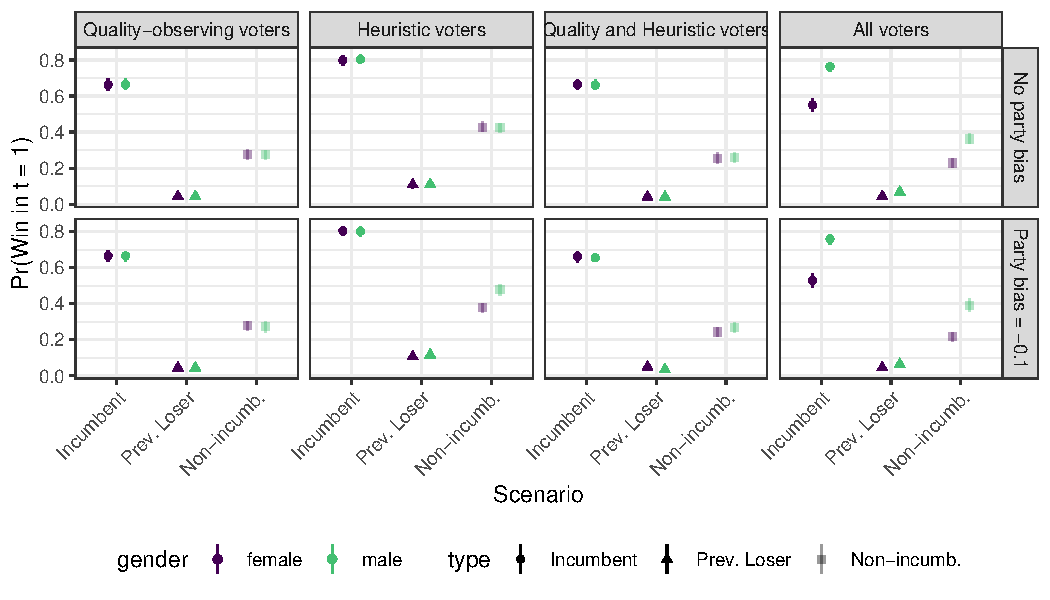
\includegraphics{../output/figures/theory_sim.pdf}
    \caption{Simulation results showing probability of election for candidate subgroups across scenarios}
    \label{fig:theory_sim}
\end{figure}

Crucially, we see no gender gaps between previous winners and previous losers across the first three scenarios. It is only when we add the biased heuristic voters into the election that we see that female candidates observe a smaller increase in their win probability as a result of incumbency when compared to men.


\pagebreak
\section{RD Robustness Checks: Main Results}

In this section, I offer a number of checks to confirm that the main results in the paper are not sensitive to different specifications of the RD design.

\subsection{Functional Form}
\label{app:rd_polynomial}

In this section, I assess the robustness of the main RD estimates with respect to functional form. Tables \ref{tab:norway_main_poly2} and \ref{tab:spain_main_poly2} below report the results from the main specification fitted with second-order polynomials. The results are consistent with the estimates from the linear specification.

\subsubsection{Norway}

\begin{table}[!h]

\caption{\label{tab:norway_main_poly2} \textbf{Difference-in-Discontinuity Estimates from Norway with Second-Order Polynomial.}}
\centering
\fontsize{9}{11}\selectfont
\begin{threeparttable}
\begin{tabular}[t]{lS[
              input-symbols=(),
              table-format=-1.3,
              table-space-text-pre    = (,
              table-space-text-post   = ),
              input-open-uncertainty  =,
              input-close-uncertainty = ,
              table-align-text-post = false]S[
              input-symbols=(),
              table-format=-1.3,
              table-space-text-pre    = (,
              table-space-text-post   = ),
              input-open-uncertainty  =,
              input-close-uncertainty = ,
              table-align-text-post = false]S[
              input-symbols=(),
              table-format=-1.3,
              table-space-text-pre    = (,
              table-space-text-post   = ),
              input-open-uncertainty  =,
              input-close-uncertainty = ,
              table-align-text-post = false]S[
              input-symbols=(),
              table-format=-1.3,
              table-space-text-pre    = (,
              table-space-text-post   = ),
              input-open-uncertainty  =,
              input-close-uncertainty = ,
              table-align-text-post = false]S[
              input-symbols=(),
              table-format=-1.3,
              table-space-text-pre    = (,
              table-space-text-post   = ),
              input-open-uncertainty  =,
              input-close-uncertainty = ,
              table-align-text-post = false]S[
              input-symbols=(),
              table-format=-1.3,
              table-space-text-pre    = (,
              table-space-text-post   = ),
              input-open-uncertainty  =,
              input-close-uncertainty = ,
              table-align-text-post = false]}
\toprule
\multicolumn{1}{c}{ } & \multicolumn{3}{c}{Run (t + 1)} & \multicolumn{3}{c}{Win (t + 1)} \\
\cmidrule(l{3pt}r{3pt}){2-4} \cmidrule(l{3pt}r{3pt}){5-7}
  & \multicolumn{1}{c}{(1)} & \multicolumn{1}{c}{(2)} & \multicolumn{1}{c}{(3)} & \multicolumn{1}{c}{(4)} & \multicolumn{1}{c}{(5)} & \multicolumn{1}{c}{(6)}\\
\midrule
Elected & 0.000 & -0.011 & 0.022 & 0.106 & 0.100 & 0.112\\
 & (0.019) & (0.016) & (0.023) & (0.017) & (0.015) & (0.022)\\
\addlinespace
Female & -0.083 & -0.080 & -0.097 & -0.025 & -0.020 & -0.032\\
 & (0.020) & (0.018) & (0.023) & (0.017) & (0.014) & (0.019)\\
\addlinespace
Elected x Female & -0.015 & 0.003 & -0.030 & -0.074 & -0.058 & -0.091\\
 & (0.032) & (0.029) & (0.038) & (0.029) & (0.025) & (0.035)\\
\addlinespace \midrule \addlinespace
Bandwidth & 0.11 & 0.22 & 0.055 & 0.091 & 0.18 & 0.045\\
BW Type & \multicolumn{1}{c}{Optimal} & \multicolumn{1}{c}{2x Opt} & \multicolumn{1}{c}{0.5x Opt} & \multicolumn{1}{c}{Optimal} & \multicolumn{1}{c}{2x Opt} & \multicolumn{1}{c}{0.5x Opt}\\
Outcome Mean & 0.576 & 0.587 & 0.565 & 0.263 & 0.262 & 0.261\\
N (left) & \multicolumn{1}{c}{5553} & \multicolumn{1}{c}{6537} & \multicolumn{1}{c}{4660} & \multicolumn{1}{c}{5314} & \multicolumn{1}{c}{6216} & \multicolumn{1}{c}{4384}\\
N (right) & \multicolumn{1}{c}{5614} & \multicolumn{1}{c}{6609} & \multicolumn{1}{c}{4709} & \multicolumn{1}{c}{5373} & \multicolumn{1}{c}{6283} & \multicolumn{1}{c}{4431}\\
\bottomrule
\end{tabular}
\begin{tablenotes}[para]
\item All estimates are reported with robust standard errors clustered at the municipality level in parentheses. Each observation is a candidate's election attempt. 'Elected' is an indicator for observations where the candidate obtained a seat in the municipal council. 'Female' is an indicator for observations identified as female. `Elected` times `Female` is the interaction between the two variables. Other coefficients not reported. Regression run on all candidates in elections between 2003 and 2015.
\end{tablenotes}
\end{threeparttable}
\end{table}

\clearpage
\subsubsection{Spain}

\begin{table}[!h]

\caption{\label{tab:spain_main_poly2} \textbf{Difference-in-Discontinuity Estimates from Spain with Second-Order Polynomial.}.}
\centering
\fontsize{9}{11}\selectfont
\begin{threeparttable}
\begin{tabular}[t]{lS[
              input-symbols=(),
              table-format=-1.3,
              table-space-text-pre    = (,
              table-space-text-post   = ),
              input-open-uncertainty  =,
              input-close-uncertainty = ,
              table-align-text-post = false]S[
              input-symbols=(),
              table-format=-1.3,
              table-space-text-pre    = (,
              table-space-text-post   = ),
              input-open-uncertainty  =,
              input-close-uncertainty = ,
              table-align-text-post = false]S[
              input-symbols=(),
              table-format=-1.3,
              table-space-text-pre    = (,
              table-space-text-post   = ),
              input-open-uncertainty  =,
              input-close-uncertainty = ,
              table-align-text-post = false]S[
              input-symbols=(),
              table-format=-1.3,
              table-space-text-pre    = (,
              table-space-text-post   = ),
              input-open-uncertainty  =,
              input-close-uncertainty = ,
              table-align-text-post = false]S[
              input-symbols=(),
              table-format=-1.3,
              table-space-text-pre    = (,
              table-space-text-post   = ),
              input-open-uncertainty  =,
              input-close-uncertainty = ,
              table-align-text-post = false]S[
              input-symbols=(),
              table-format=-1.3,
              table-space-text-pre    = (,
              table-space-text-post   = ),
              input-open-uncertainty  =,
              input-close-uncertainty = ,
              table-align-text-post = false]}
\toprule
\multicolumn{1}{c}{ } & \multicolumn{3}{c}{Run (in t+1)} & \multicolumn{3}{c}{Win (in t+1)} \\
\cmidrule(l{3pt}r{3pt}){2-4} \cmidrule(l{3pt}r{3pt}){5-7}
  & \multicolumn{1}{c}{(1)} & \multicolumn{1}{c}{(2)} & \multicolumn{1}{c}{(3)} & \multicolumn{1}{c}{(4)} & \multicolumn{1}{c}{(5)} & \multicolumn{1}{c}{(6)}\\
\midrule
Elected & 0.095 & 0.116 & 0.075 & 0.076 & 0.087 & 0.074\\
 & (0.020) & (0.014) & (0.029) & (0.014) & (0.010) & (0.020)\\
\addlinespace
Female & -0.014 & -0.014 & 0.008 & -0.027 & -0.030 & -0.037\\
 & (0.023) & (0.017) & (0.032) & (0.015) & (0.010) & (0.021)\\
\addlinespace
Elected x Female & 0.043 & 0.021 & 0.011 & 0.045 & 0.053 & 0.056\\
 & (0.032) & (0.023) & (0.046) & (0.022) & (0.016) & (0.031)\\
\addlinespace \midrule \addlinespace
Bandwidth & 0.036 & 0.072 & 0.018 & 0.059 & 0.12 & 0.029\\
BW Type & \multicolumn{1}{c}{Optimal} & \multicolumn{1}{c}{2x Opt} & \multicolumn{1}{c}{0.5x Opt} & \multicolumn{1}{c}{Optimal} & \multicolumn{1}{c}{2x Opt} & \multicolumn{1}{c}{0.5x Opt}\\
Outcome Mean & 0.487 & 0.481 & 0.486 & 0.253 & 0.244 & 0.255\\
N (left) & \multicolumn{1}{c}{16564} & \multicolumn{1}{c}{28924} & \multicolumn{1}{c}{8917} & \multicolumn{1}{c}{24559} & \multicolumn{1}{c}{40700} & \multicolumn{1}{c}{13705}\\
N (right) & \multicolumn{1}{c}{16568} & \multicolumn{1}{c}{29555} & \multicolumn{1}{c}{8708} & \multicolumn{1}{c}{25132} & \multicolumn{1}{c}{40620} & \multicolumn{1}{c}{13587}\\
\bottomrule
\end{tabular}
\begin{tablenotes}[para]
\item All estimates are reported with robust standard errors clustered at the municipality level in parentheses. Each observation is a candidate's election attempt. 'Elected' is an indicator for observations where the candidate obtained a seat in the municipal council. 'Female' is an indicator for observations identified as female. `Elected` times `Female` is the interaction between the two variables. Other coefficients not reported. Regression run on all candidates in elections between 2003 and 2015.
\end{tablenotes}
\end{threeparttable}
\end{table}

\clearpage
\subsection{Bandwidth Sensitivity}
\label{app:bandwidth_sensitivity}

Tables \ref{tab:norway_main} and \ref{tab:spain_main} report results of the heterogeneity-in-discontinuity specification with optimal bandwidth as selected by \citet{calonico2014} on the full sample, along with one-half and double that bandwidth. Below, I plot the coefficient estimates of interest with additional bandwidth parameters to ascertain that the results are robust to the choice of bandwidth.

\subsubsection{Norway}
\begin{figure}[!htb]
    \centering
    \begin{subfigure}[t]{0.48\textwidth}
    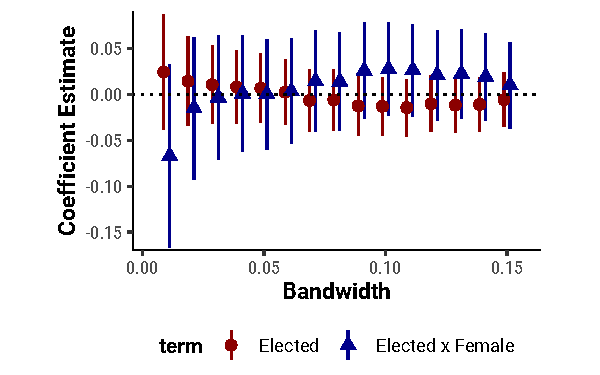
\includegraphics[width = 1 \textwidth]{../output/figures/norway_run_again_bw.pdf}
    \caption{Running in $t+1$}
    \end{subfigure}%
    \begin{subfigure}[t]{0.48\textwidth}
    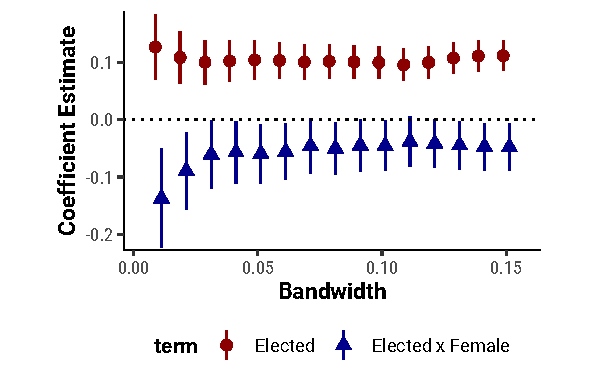
\includegraphics[width = 1 \textwidth]{../output/figures/norway_win_again_bw.pdf}
    \caption{Winning in $t+1$}
    \end{subfigure}
    \caption{\textbf{Bandwidth Sensitivity Check (Norway).} The plot shows the RD coefficients for `Elected` and `Elected x Female` in the case of Norway for different bandwidth choices.}
    \label{fig:norway_bw_sens}
\end{figure}

\clearpage
\subsubsection{Spain}
\begin{figure}[!htb]
    \centering
    \begin{subfigure}[t]{0.48\textwidth}
    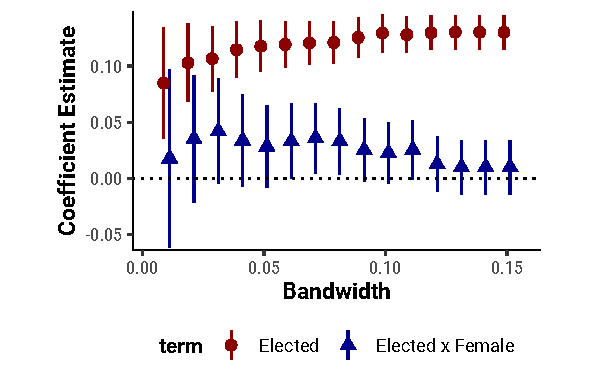
\includegraphics[width = 1 \textwidth]{../output/figures/spain_run_again_bw.pdf}
    \caption{Running in $t+1$}
    \end{subfigure}%
    \begin{subfigure}[t]{0.48\textwidth}
    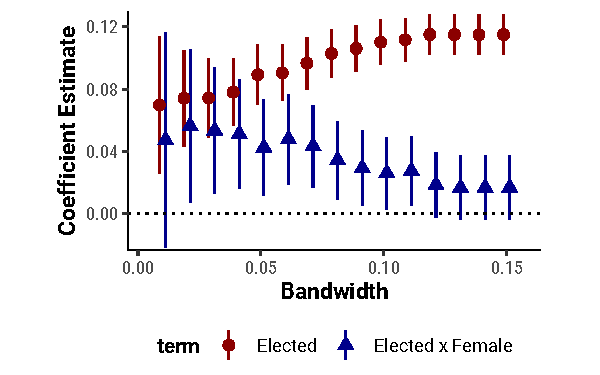
\includegraphics[width = 1 \textwidth]{../output/figures/spain_win_again_bw.pdf}
    \caption{Winning in $t+1$}
    \end{subfigure}
    \caption{\textbf{Bandwidth Sensitivity Check (Spain).} The plot shows the RD coefficients for `Elected` and `Elected x Female` in the case of Spain for different bandwidth choices.}
    \label{fig:spain_bw_sens}
\end{figure}

\clearpage
\pagebreak

\subsection{Kernel Choice}
\label{app:kernelchoice}

Below, I present estimates from the main specification with triangular, rather than uniform kernels. The results are very similar to the preferred estimates in the main body of the paper in both countries.

\begin{table}[!h]

\caption{\label{tab:norway_main_tri} \textbf{Difference-in-Discontinuity Estimates For Incumbency Advantage In Norwegian Municipalities, with triangular kernels.} Women Face Diminished Incumbency Effect On Winning Again.}
\centering
\fontsize{9}{11}\selectfont
\begin{threeparttable}
\begin{tabular}[t]{lS[
              input-symbols=(),
              table-format=-1.3,
              table-space-text-pre    = (,
              table-space-text-post   = ),
              input-open-uncertainty  =,
              input-close-uncertainty = ,
              table-align-text-post = false]S[
              input-symbols=(),
              table-format=-1.3,
              table-space-text-pre    = (,
              table-space-text-post   = ),
              input-open-uncertainty  =,
              input-close-uncertainty = ,
              table-align-text-post = false]S[
              input-symbols=(),
              table-format=-1.3,
              table-space-text-pre    = (,
              table-space-text-post   = ),
              input-open-uncertainty  =,
              input-close-uncertainty = ,
              table-align-text-post = false]S[
              input-symbols=(),
              table-format=-1.3,
              table-space-text-pre    = (,
              table-space-text-post   = ),
              input-open-uncertainty  =,
              input-close-uncertainty = ,
              table-align-text-post = false]S[
              input-symbols=(),
              table-format=-1.3,
              table-space-text-pre    = (,
              table-space-text-post   = ),
              input-open-uncertainty  =,
              input-close-uncertainty = ,
              table-align-text-post = false]S[
              input-symbols=(),
              table-format=-1.3,
              table-space-text-pre    = (,
              table-space-text-post   = ),
              input-open-uncertainty  =,
              input-close-uncertainty = ,
              table-align-text-post = false]}
\toprule
\multicolumn{1}{c}{ } & \multicolumn{3}{c}{Run (t + 1)} & \multicolumn{3}{c}{Win (t + 1)} \\
\cmidrule(l{3pt}r{3pt}){2-4} \cmidrule(l{3pt}r{3pt}){5-7}
  & \multicolumn{1}{c}{(1)} & \multicolumn{1}{c}{(2)} & \multicolumn{1}{c}{(3)} & \multicolumn{1}{c}{(4)} & \multicolumn{1}{c}{(5)} & \multicolumn{1}{c}{(6)}\\
\midrule
Elected & 0.011 & -0.003 & 0.018 & 0.106 & 0.102 & 0.112\\
 & (0.020) & (0.017) & (0.025) & (0.018) & (0.015) & (0.022)\\
\addlinespace
Female & -0.089 & -0.089 & -0.081 & -0.031 & -0.030 & -0.022\\
 & (0.023) & (0.019) & (0.027) & (0.019) & (0.016) & (0.024)\\
\addlinespace
Elected x Female & -0.019 & 0.007 & -0.040 & -0.071 & -0.053 & -0.102\\
 & (0.035) & (0.030) & (0.041) & (0.030) & (0.025) & (0.037)\\
\addlinespace \midrule \addlinespace
Bandwidth & 0.054 & 0.11 & 0.027 & 0.05 & 0.099 & 0.025\\
BW Type & \multicolumn{1}{c}{Optimal} & \multicolumn{1}{c}{2x Opt} & \multicolumn{1}{c}{0.5x Opt} & \multicolumn{1}{c}{Optimal} & \multicolumn{1}{c}{2x Opt} & \multicolumn{1}{c}{0.5x Opt}\\
Outcome Mean & 0.564 & 0.575 & 0.551 & 0.261 & 0.263 & 0.257\\
N (left) & \multicolumn{1}{c}{4617} & \multicolumn{1}{c}{5529} & \multicolumn{1}{c}{3667} & \multicolumn{1}{c}{4502} & \multicolumn{1}{c}{5428} & \multicolumn{1}{c}{3549}\\
N (right) & \multicolumn{1}{c}{4666} & \multicolumn{1}{c}{5590} & \multicolumn{1}{c}{3711} & \multicolumn{1}{c}{4551} & \multicolumn{1}{c}{5489} & \multicolumn{1}{c}{3592}\\
\bottomrule
\end{tabular}
\begin{tablenotes}[para]
\item All estimates are reported with robust standard errors clustered at the municipality level in parentheses. Each observation is a candidate's election attempt. 'Elected' is an indicator for observations where the candidate obtained a seat in the municipal council. 'Female' is an indicator for observations identified as female. `Elected` times `Female` is the interaction between the two variables. Other coefficients not reported. Regression run on all candidates in elections between 2003 and 2015.
\end{tablenotes}
\end{threeparttable}
\end{table}

\begin{table}[!h]

\caption{\label{tab:spain_main_tri} \textbf{Difference-in-Discontinuity Estimates For Incumbency Advantage In Spanish Municipalities, with triangular kernels}. Women enjoy a larger effect of winning on their probability to win again.}
\centering
\fontsize{9}{11}\selectfont
\begin{threeparttable}
\begin{tabular}[t]{lS[
              input-symbols=(),
              table-format=-1.3,
              table-space-text-pre    = (,
              table-space-text-post   = ),
              input-open-uncertainty  =,
              input-close-uncertainty = ,
              table-align-text-post = false]S[
              input-symbols=(),
              table-format=-1.3,
              table-space-text-pre    = (,
              table-space-text-post   = ),
              input-open-uncertainty  =,
              input-close-uncertainty = ,
              table-align-text-post = false]S[
              input-symbols=(),
              table-format=-1.3,
              table-space-text-pre    = (,
              table-space-text-post   = ),
              input-open-uncertainty  =,
              input-close-uncertainty = ,
              table-align-text-post = false]S[
              input-symbols=(),
              table-format=-1.3,
              table-space-text-pre    = (,
              table-space-text-post   = ),
              input-open-uncertainty  =,
              input-close-uncertainty = ,
              table-align-text-post = false]S[
              input-symbols=(),
              table-format=-1.3,
              table-space-text-pre    = (,
              table-space-text-post   = ),
              input-open-uncertainty  =,
              input-close-uncertainty = ,
              table-align-text-post = false]S[
              input-symbols=(),
              table-format=-1.3,
              table-space-text-pre    = (,
              table-space-text-post   = ),
              input-open-uncertainty  =,
              input-close-uncertainty = ,
              table-align-text-post = false]}
\toprule
\multicolumn{1}{c}{ } & \multicolumn{3}{c}{Run (t + 1)} & \multicolumn{3}{c}{Win (t + 1)} \\
\cmidrule(l{3pt}r{3pt}){2-4} \cmidrule(l{3pt}r{3pt}){5-7}
  & \multicolumn{1}{c}{(1)} & \multicolumn{1}{c}{(2)} & \multicolumn{1}{c}{(3)} & \multicolumn{1}{c}{(4)} & \multicolumn{1}{c}{(5)} & \multicolumn{1}{c}{(6)}\\
\midrule
Elected & 0.103 & 0.116 & 0.093 & 0.075 & 0.088 & 0.074\\
 & (0.016) & (0.011) & (0.022) & (0.013) & (0.009) & (0.019)\\
\addlinespace
Female & -0.018 & -0.027 & -0.005 & -0.030 & -0.026 & -0.030\\
 & (0.018) & (0.013) & (0.025) & (0.014) & (0.010) & (0.019)\\
\addlinespace
Elected x Female & 0.038 & 0.031 & 0.020 & 0.055 & 0.046 & 0.049\\
 & (0.025) & (0.018) & (0.035) & (0.021) & (0.015) & (0.029)\\
\addlinespace \midrule \addlinespace
Bandwidth & 0.032 & 0.064 & 0.016 & 0.035 & 0.071 & 0.018\\
BW Type & \multicolumn{1}{c}{Optimal} & \multicolumn{1}{c}{2x Opt} & \multicolumn{1}{c}{0.5x Opt} & \multicolumn{1}{c}{Optimal} & \multicolumn{1}{c}{2x Opt} & \multicolumn{1}{c}{0.5x Opt}\\
Outcome Mean & 0.486 & 0.483 & 0.485 & 0.256 & 0.251 & 0.254\\
N (left) & \multicolumn{1}{c}{14840} & \multicolumn{1}{c}{26294} & \multicolumn{1}{c}{7984} & \multicolumn{1}{c}{16223} & \multicolumn{1}{c}{28426} & \multicolumn{1}{c}{8726}\\
N (right) & \multicolumn{1}{c}{14729} & \multicolumn{1}{c}{26886} & \multicolumn{1}{c}{7825} & \multicolumn{1}{c}{16159} & \multicolumn{1}{c}{29072} & \multicolumn{1}{c}{8530}\\
\bottomrule
\end{tabular}
\begin{tablenotes}[para]
\item All estimates are reported with robust standard errors clustered at the municipality level in parentheses.
\end{tablenotes}
\end{threeparttable}
\end{table}

\clearpage
\pagebreak

\subsection{Estimates without Fixed Effects}
\label{app:nofe}

Below, I show results from heterogeneity-in-discontinuity specifications mirroring the main specification, but estimated without fixed effects. This specification matches the heterogeneity-in-discontinuities estimator discussed in \citet{bansak2022}. The results are very similar.

\begin{table}[!h]

\caption{\label{tab:norway_main_nofe} \textbf{Difference-in-Discontinuity Estimates For Incumbency Advantage In Norwegian Municipalities, without fixed effects.} Women Face Diminished Incumbency Effect On Winning Again.}
\centering
\fontsize{9}{11}\selectfont
\begin{threeparttable}
\begin{tabular}[t]{lS[
              input-symbols=(),
              table-format=-1.3,
              table-space-text-pre    = (,
              table-space-text-post   = ),
              input-open-uncertainty  =,
              input-close-uncertainty = ,
              table-align-text-post = false]S[
              input-symbols=(),
              table-format=-1.3,
              table-space-text-pre    = (,
              table-space-text-post   = ),
              input-open-uncertainty  =,
              input-close-uncertainty = ,
              table-align-text-post = false]S[
              input-symbols=(),
              table-format=-1.3,
              table-space-text-pre    = (,
              table-space-text-post   = ),
              input-open-uncertainty  =,
              input-close-uncertainty = ,
              table-align-text-post = false]S[
              input-symbols=(),
              table-format=-1.3,
              table-space-text-pre    = (,
              table-space-text-post   = ),
              input-open-uncertainty  =,
              input-close-uncertainty = ,
              table-align-text-post = false]S[
              input-symbols=(),
              table-format=-1.3,
              table-space-text-pre    = (,
              table-space-text-post   = ),
              input-open-uncertainty  =,
              input-close-uncertainty = ,
              table-align-text-post = false]S[
              input-symbols=(),
              table-format=-1.3,
              table-space-text-pre    = (,
              table-space-text-post   = ),
              input-open-uncertainty  =,
              input-close-uncertainty = ,
              table-align-text-post = false]}
\toprule
\multicolumn{1}{c}{ } & \multicolumn{3}{c}{Run (t + 1)} & \multicolumn{3}{c}{Win (t + 1)} \\
\cmidrule(l{3pt}r{3pt}){2-4} \cmidrule(l{3pt}r{3pt}){5-7}
  & \multicolumn{1}{c}{(1)} & \multicolumn{1}{c}{(2)} & \multicolumn{1}{c}{(3)} & \multicolumn{1}{c}{(4)} & \multicolumn{1}{c}{(5)} & \multicolumn{1}{c}{(6)}\\
\midrule
Elected & -0.002 & -0.014 & 0.014 & 0.110 & 0.104 & 0.110\\
 & (0.019) & (0.016) & (0.023) & (0.017) & (0.015) & (0.021)\\
\addlinespace
Female & -0.106 & -0.099 & -0.092 & -0.025 & -0.023 & -0.022\\
 & (0.021) & (0.018) & (0.026) & (0.017) & (0.015) & (0.021)\\
\addlinespace
Elected x Female & 0.008 & 0.032 & -0.031 & -0.069 & -0.050 & -0.099\\
 & (0.033) & (0.028) & (0.039) & (0.028) & (0.024) & (0.035)\\
\addlinespace \midrule \addlinespace
Bandwidth & 0.054 & 0.11 & 0.027 & 0.05 & 0.099 & 0.025\\
BW Type & \multicolumn{1}{c}{Optimal} & \multicolumn{1}{c}{2x Opt} & \multicolumn{1}{c}{0.5x Opt} & \multicolumn{1}{c}{Optimal} & \multicolumn{1}{c}{2x Opt} & \multicolumn{1}{c}{0.5x Opt}\\
Outcome Mean & 0.564 & 0.575 & 0.551 & 0.261 & 0.263 & 0.257\\
N (left) & \multicolumn{1}{c}{4617} & \multicolumn{1}{c}{5529} & \multicolumn{1}{c}{3667} & \multicolumn{1}{c}{4502} & \multicolumn{1}{c}{5428} & \multicolumn{1}{c}{3549}\\
N (right) & \multicolumn{1}{c}{4666} & \multicolumn{1}{c}{5590} & \multicolumn{1}{c}{3711} & \multicolumn{1}{c}{4551} & \multicolumn{1}{c}{5489} & \multicolumn{1}{c}{3592}\\
\bottomrule
\end{tabular}
\begin{tablenotes}[para]
\item All estimates are reported with robust standard errors clustered at the municipality level in parentheses. Each observation is a candidate's election attempt. 'Elected' is an indicator for observations where the candidate obtained a seat in the municipal council. 'Female' is an indicator for observations identified as female. `Elected` times `Female` is the interaction between the two variables. Other coefficients not reported. Regression run on all candidates in elections between 2003 and 2015.
\end{tablenotes}
\end{threeparttable}
\end{table}

\begin{table}[!h]

\caption{\label{tab:spain_main_nofe} \textbf{Difference-in-Discontinuity Estimates For Incumbency Advantage In Spanish Municipalities, Without Fixed Effects}. Women enjoy a larger effect of winning on their probability to win again.}
\centering
\fontsize{9}{11}\selectfont
\begin{threeparttable}
\begin{tabular}[t]{lS[
              input-symbols=(),
              table-format=-1.3,
              table-space-text-pre    = (,
              table-space-text-post   = ),
              input-open-uncertainty  =,
              input-close-uncertainty = ,
              table-align-text-post = false]S[
              input-symbols=(),
              table-format=-1.3,
              table-space-text-pre    = (,
              table-space-text-post   = ),
              input-open-uncertainty  =,
              input-close-uncertainty = ,
              table-align-text-post = false]S[
              input-symbols=(),
              table-format=-1.3,
              table-space-text-pre    = (,
              table-space-text-post   = ),
              input-open-uncertainty  =,
              input-close-uncertainty = ,
              table-align-text-post = false]S[
              input-symbols=(),
              table-format=-1.3,
              table-space-text-pre    = (,
              table-space-text-post   = ),
              input-open-uncertainty  =,
              input-close-uncertainty = ,
              table-align-text-post = false]S[
              input-symbols=(),
              table-format=-1.3,
              table-space-text-pre    = (,
              table-space-text-post   = ),
              input-open-uncertainty  =,
              input-close-uncertainty = ,
              table-align-text-post = false]S[
              input-symbols=(),
              table-format=-1.3,
              table-space-text-pre    = (,
              table-space-text-post   = ),
              input-open-uncertainty  =,
              input-close-uncertainty = ,
              table-align-text-post = false]}
\toprule
\multicolumn{1}{c}{ } & \multicolumn{3}{c}{Run (t + 1)} & \multicolumn{3}{c}{Win (t + 1)} \\
\cmidrule(l{3pt}r{3pt}){2-4} \cmidrule(l{3pt}r{3pt}){5-7}
  & \multicolumn{1}{c}{(1)} & \multicolumn{1}{c}{(2)} & \multicolumn{1}{c}{(3)} & \multicolumn{1}{c}{(4)} & \multicolumn{1}{c}{(5)} & \multicolumn{1}{c}{(6)}\\
\midrule
Elected & 0.109 & 0.120 & 0.097 & 0.074 & 0.097 & 0.080\\
 & (0.014) & (0.010) & (0.020) & (0.012) & (0.008) & (0.017)\\
\addlinespace
Female & -0.020 & -0.030 & -0.010 & -0.029 & -0.023 & -0.026\\
 & (0.016) & (0.012) & (0.022) & (0.013) & (0.009) & (0.018)\\
\addlinespace
Elected x Female & 0.034 & 0.031 & 0.019 & 0.054 & 0.043 & 0.054\\
 & (0.023) & (0.017) & (0.032) & (0.019) & (0.014) & (0.027)\\
\addlinespace \midrule \addlinespace
Bandwidth & 0.032 & 0.064 & 0.016 & 0.035 & 0.071 & 0.018\\
BW Type & \multicolumn{1}{c}{Optimal} & \multicolumn{1}{c}{2x Opt} & \multicolumn{1}{c}{0.5x Opt} & \multicolumn{1}{c}{Optimal} & \multicolumn{1}{c}{2x Opt} & \multicolumn{1}{c}{0.5x Opt}\\
Outcome Mean & 0.486 & 0.483 & 0.485 & 0.256 & 0.251 & 0.254\\
N (left) & \multicolumn{1}{c}{14840} & \multicolumn{1}{c}{26294} & \multicolumn{1}{c}{7984} & \multicolumn{1}{c}{16223} & \multicolumn{1}{c}{28426} & \multicolumn{1}{c}{8726}\\
N (right) & \multicolumn{1}{c}{14729} & \multicolumn{1}{c}{26886} & \multicolumn{1}{c}{7825} & \multicolumn{1}{c}{16159} & \multicolumn{1}{c}{29072} & \multicolumn{1}{c}{8530}\\
\bottomrule
\end{tabular}
\begin{tablenotes}[para]
\item All estimates are reported with robust standard errors clustered at the municipality level in parentheses.
\end{tablenotes}
\end{threeparttable}
\end{table}

\clearpage

\subsection{Estimates conditional on running again}

The results below report the gender gap in the effect of winning again \emph{conditional} on running again. These results should be treated with caution, as the decision to run again is also affected by the treatment. Nonetheless, they can help ease concerns about alternative explanations of the gender gaprelated to differential selection into running again after winning office.

\begin{table}

\caption{\label{tab:norway_main} \textbf{Difference-in-Discontinuity Estimates For Incumbency Advantage In Norwegian Municipalities, Conditional on Running Again.}}
\centering
\fontsize{9}{11}\selectfont
\begin{threeparttable}
\begin{tabular}[t]{lS[
              input-symbols=(),
              table-format=-1.3,
              table-space-text-pre    = (,
              table-space-text-post   = ),
              input-open-uncertainty  =,
              input-close-uncertainty = ,
              table-align-text-post = false]S[
              input-symbols=(),
              table-format=-1.3,
              table-space-text-pre    = (,
              table-space-text-post   = ),
              input-open-uncertainty  =,
              input-close-uncertainty = ,
              table-align-text-post = false]S[
              input-symbols=(),
              table-format=-1.3,
              table-space-text-pre    = (,
              table-space-text-post   = ),
              input-open-uncertainty  =,
              input-close-uncertainty = ,
              table-align-text-post = false]}
\toprule
\multicolumn{1}{c}{ } & \multicolumn{3}{c}{Win (t + 1)} \\
\cmidrule(l{3pt}r{3pt}){2-4}
  & \multicolumn{1}{c}{(1)} & \multicolumn{1}{c}{(2)} & \multicolumn{1}{c}{(3)}\\
\midrule
Elected & 0.179 & 0.182 & 0.163\\
 & (0.023) & (0.020) & (0.028)\\
\addlinespace
Female & 0.011 & 0.014 & -0.002\\
 & (0.028) & (0.022) & (0.033)\\
\addlinespace
Elected x Female & -0.073 & -0.061 & -0.068\\
 & (0.040) & (0.033) & (0.050)\\
\addlinespace \midrule \addlinespace
Bandwidth & 0.062 & 0.12 & 0.031\\
BW Type & \multicolumn{1}{c}{Optimal} & \multicolumn{1}{c}{2x Opt} & \multicolumn{1}{c}{0.5x Opt}\\
Outcome Mean & 0.464 & 0.457 & 0.467\\
N (left) & \multicolumn{1}{c}{2727} & \multicolumn{1}{c}{3288} & \multicolumn{1}{c}{2146}\\
N (right) & \multicolumn{1}{c}{2734} & \multicolumn{1}{c}{3316} & \multicolumn{1}{c}{2154}\\
\bottomrule
\end{tabular}
\begin{tablenotes}[para]
\item All estimates are reported with robust standard errors clustered at the municipality level in parentheses. 
\end{tablenotes}
\end{threeparttable}
\end{table}

\begin{table}

\caption{\label{tab:spain_main_conditional} \textbf{Difference-in-Discontinuity Estimates For Incumbency Advantage In Spanish Municipalities, Conditional On Running Again}.}
\centering
\fontsize{9}{11}\selectfont
\begin{threeparttable}
\begin{tabular}[t]{lS[
              input-symbols=(),
              table-format=-1.3,
              table-space-text-pre    = (,
              table-space-text-post   = ),
              input-open-uncertainty  =,
              input-close-uncertainty = ,
              table-align-text-post = false]S[
              input-symbols=(),
              table-format=-1.3,
              table-space-text-pre    = (,
              table-space-text-post   = ),
              input-open-uncertainty  =,
              input-close-uncertainty = ,
              table-align-text-post = false]S[
              input-symbols=(),
              table-format=-1.3,
              table-space-text-pre    = (,
              table-space-text-post   = ),
              input-open-uncertainty  =,
              input-close-uncertainty = ,
              table-align-text-post = false]}
\toprule
\multicolumn{1}{c}{ } & \multicolumn{3}{c}{Win (t + 1)} \\
\cmidrule(l{3pt}r{3pt}){2-4}
  & \multicolumn{1}{c}{(1)} & \multicolumn{1}{c}{(2)} & \multicolumn{1}{c}{(3)}\\
\midrule
Elected & 0.031 & 0.063 & 0.042\\
 & (0.020) & (0.014) & (0.028)\\
\addlinespace
Female & -0.046 & -0.024 & -0.051\\
 & (0.024) & (0.017) & (0.032)\\
\addlinespace
Elected x Female & 0.076 & 0.054 & 0.089\\
 & (0.032) & (0.023) & (0.043)\\
\addlinespace \midrule \addlinespace
Bandwidth & 0.036 & 0.072 & 0.018\\
BW Type & \multicolumn{1}{c}{Optimal} & \multicolumn{1}{c}{2x Opt} & \multicolumn{1}{c}{0.5x Opt}\\
Outcome Mean & 0.525 & 0.521 & 0.523\\
N (left) & \multicolumn{1}{c}{6884} & \multicolumn{1}{c}{11825} & \multicolumn{1}{c}{3727}\\
N (right) & \multicolumn{1}{c}{9099} & \multicolumn{1}{c}{16099} & \multicolumn{1}{c}{4759}\\
\bottomrule
\end{tabular}
\begin{tablenotes}[para]
\item All estimates are reported with robust standard errors clustered at the municipality level in parentheses.
\end{tablenotes}
\end{threeparttable}
\end{table}

\clearpage


\pagebreak

\section{RD Robustness Checks: Identification Assumptions}

In this section, I discuss additional checks verifying that there is no sorting around the RD threshold.

\subsection{Continuity Around Threshold}
\label{app:density_checks}

In order for the regression discontinuity design to identify the causal effect of being elected within each gender, the key assumption is continuity around the threshold -- that is, observations on either side of the threshold are comparable in all respects except for the treatment assignment and the outcome.

\begin{figure}[!htb]
    \centering
    \begin{subfigure}[t]{0.48\textwidth}
    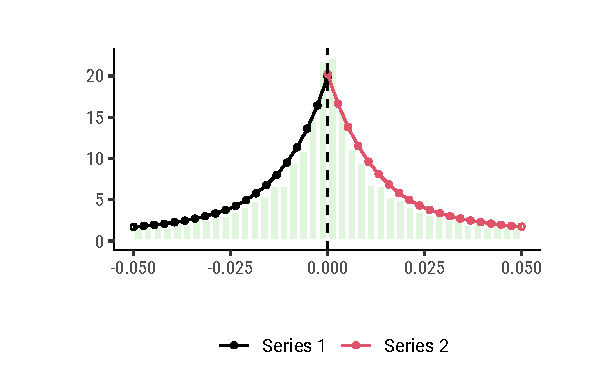
\includegraphics[width = 1 \textwidth]{../output/figures/norway_density.pdf}
    \caption{Norway}
    \end{subfigure}%
    \begin{subfigure}[t]{0.48\textwidth}
    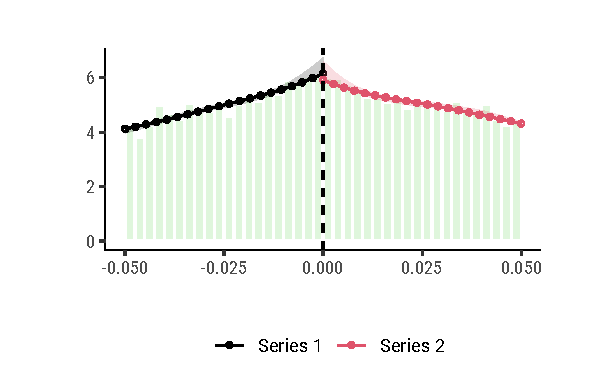
\includegraphics[width = 1 \textwidth]{../output/figures/spain_density.pdf}
    \caption{Spain}
    \end{subfigure}
    \caption{\textbf{No Discontinuity in Running Variable Density Around Threshold.} The plots show a local linear regression fitted on the density of the running variable.}
    \label{fig:continuity_assumption}
\end{figure}

\pagebreak
\subsection{Continuity in Share Of Female Candidates}
\label{app:density_covariates}

Similarly, if there is no sorting around the threshold, we should observe no discontinuous jump in the share of female candidates at the threshold. Figure \ref{fig:density_covariates} confirms that this is the case.

\begin{figure}[!htb]
    \centering
    \begin{subfigure}[t]{0.48\textwidth}
    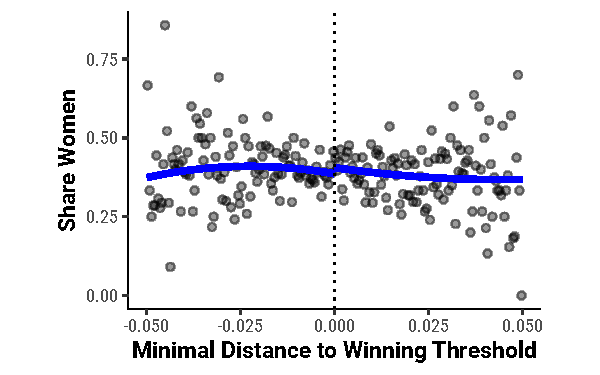
\includegraphics[width = 1 \textwidth]{../output/figures/norway_share_female.pdf}
    \caption{Norway}
    \end{subfigure}%
    \begin{subfigure}[t]{0.48\textwidth}
    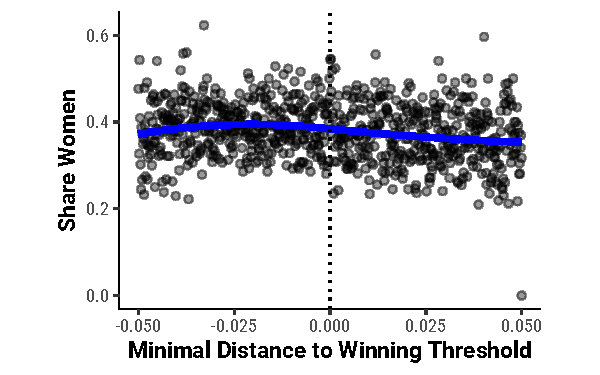
\includegraphics[width = 1 \textwidth]{../output/figures/spain_share_female.pdf}
    \caption{Spain}
    \end{subfigure}
    \caption{\textbf{No Discontinuity in Share Of Female Candidates Around Threshold.} The plots show a local quadratic regression predicting the share of female candidates around the threshold.}
    \label{fig:density_covariates}
\end{figure}

\pagebreak


\section{Identifying Close Winners and Losers under Proportional Representation}
\label{app:pr_running}

In the context of PR elections, constructing the running variable and identifying which candidates came close to barely losing or barely winning is not as straightforward as in the archetypal plurality case \citep{lee2001a,lee2008, fiva2016,fiva2018b}. These individual-level measures are different from \citet{blais2009} and \citet{cox2020}, who measure competitiveness at the district level.



% Make clear that although the overall empirical strategy for the two cases is near identical, the way the running variable is constructed is different -- much in the same way we would construct different running variables for plurality and PR.

\paragraph*{Norway (open-list).} I am constructing the margin of victory (running variable) following \citet{fiva2018a}. Effectively, the strategy identifies bare winners and bare winners within each party as those candidates who have just about gained enough preference votes (or just about missed out on enough preference votes) to be elected (to be defeated).\footnote{One issue with this choice of running variable is that the observations closest to either side of the threshold are likely to have greater population and district magnitude. This follows from the distribution of personal votes across the number of candidates within a list -- very tight margins (e.g. less than a percentage point) are more likely when there are many candidates with similar, small shares of personal votes. Although this issue does not confound the LATE estimate at the threshold (since units do not sort according to treatment status), it does pose a problem of adequate functional form for outcomes such as personal vote shares in $t+1$. See Appendix \ref{app:norway_pv_estimation} for more details.} The as-if random element comes from the distribution of preference votes across candidates of the same list. Following Fiva and Rohr's notation, the margin of victory for candidate $i$ on party list $l$ is defined as:

\begin{equation}
MV_{il} = \begin{cases}
\frac{Poll_{il} - Poll_{l}^{S_l + 1}}{PartyVotes_l} \ \text{if elected} \\
\frac{Poll_{il} - Poll_{l}^{S_l}}{PartyVotes_l} \ \text{if not elected} \\
\end{cases}
\end{equation}

where $Poll_{il}$ denotes candidates' personal vote share, $Poll_l^{S_l + 1}$ denotes the vote share of party $l$'s first loser, and $Poll_l^S$ denotes the vote share of party $l$'s last winner. $PartyVotes_l$ is the total number of votes cast for party $l$. In other words, I construct the margin of victory  using the difference in personal votes between candidate $i$ and the vote threshold to winning a seat, normalized by the total number of votes the party obtained.

I construct the running variable in the same way for my supplementary analysis of county-level elections in Poland.

\paragraph*{Spain (closed-list).} I construct the running variable following \cite{folke2014} and calculate a `minimum distance' to winning (or losing) an extra seat for the legislator's party.\footnote{Note, in the original application of this method, the algorithm does not account for electoral thresholds below which parties are excluded from the seat allocation altogether. In the Spanish case, there is a 4\% threshold. However, because of low district magnitudes, the \emph{effective} threshold necessary for parties to clear to win seats, is typically higher than this. Still, I exclude candidates from lists that scored less than 10\% in an election from my sample to ensure that the minimum distance calculated is not affected by the legal threshold.} The as-if random element comes from the discontinuous translation from parties' vote shares to a discrete number of seats, where a small perturbation in the vote share may lead to a different candidate winning the last available seat. I compute the smallest change in the vote share distribution that would cause a party to either lose or win an additional seat. In other words, in each municipal election, I identify the closest winner (the last seat assigned) and the closest loser (the first candidate to miss out on a seat), and calculate the necessary change vote share to flip the last seat from the winner to the loser.

Note that the setup of the running variable in the two countries identifies bare winners and bare losers in different ways.
%In Norway, the running variable is defined with respect to the within-party distribution of votes: the pair of barely losing and barely winning candidates therefore appears in every party list in every election, unless a party has obtained no seats. In Spain, on the other hand, I can only compare the barely losing candidate of one list with the barely winning candidate of another list (as I am exploiting the as-if random assignment of the last seat between parties). This means that the \emph{dimensions} of the running variable are not comparable to one another.
However, since my quantity of interest is the LATE subgroup estimate at the threshold, both running variables identify bare winners and bare losers in their respective electoral context. It is typical for different electoral systems to require different operationalisations of the margin of victory. See \citet{eggers2015a} for plurality, \citet{folke2014,fiva2018b,fiva2016} for closed-list PR, \citet{folke2016d,fiva2018a} for open-list PR. Moreover, since I am using party-by-year fixed effects in my specifications, my results in Norway are also not driven by selection of candidates into specific parties.

\pagebreak
\clearpage

\section{Testing the Gender Gap Across Systems And Countries}
\label{app:case_extension}

\subsection{Same Country, Different Electoral System: Likely No Gender Gap}


\begin{table}

\caption{\label{tab:norway_national} \textbf{Probabilities of Winning Re-Election in Norway's National Elections (Difference-in-Differences).} }
\centering
\fontsize{9}{11}\selectfont
\begin{threeparttable}
\begin{tabular}[t]{lS[
              input-symbols=(),
              table-format=-2.3,
              table-space-text-pre    = (,
              table-space-text-post   = ),
              input-open-uncertainty  =,
              input-close-uncertainty = ,
              table-align-text-post = false]S[
              input-symbols=(),
              table-format=-2.3,
              table-space-text-pre    = (,
              table-space-text-post   = ),
              input-open-uncertainty  =,
              input-close-uncertainty = ,
              table-align-text-post = false]S[
              input-symbols=(),
              table-format=-2.3,
              table-space-text-pre    = (,
              table-space-text-post   = ),
              input-open-uncertainty  =,
              input-close-uncertainty = ,
              table-align-text-post = false]S[
              input-symbols=(),
              table-format=-2.3,
              table-space-text-pre    = (,
              table-space-text-post   = ),
              input-open-uncertainty  =,
              input-close-uncertainty = ,
              table-align-text-post = false]S[
              input-symbols=(),
              table-format=-2.3,
              table-space-text-pre    = (,
              table-space-text-post   = ),
              input-open-uncertainty  =,
              input-close-uncertainty = ,
              table-align-text-post = false]S[
              input-symbols=(),
              table-format=-2.3,
              table-space-text-pre    = (,
              table-space-text-post   = ),
              input-open-uncertainty  =,
              input-close-uncertainty = ,
              table-align-text-post = false]S[
              input-symbols=(),
              table-format=-2.3,
              table-space-text-pre    = (,
              table-space-text-post   = ),
              input-open-uncertainty  =,
              input-close-uncertainty = ,
              table-align-text-post = false]S[
              input-symbols=(),
              table-format=-2.3,
              table-space-text-pre    = (,
              table-space-text-post   = ),
              input-open-uncertainty  =,
              input-close-uncertainty = ,
              table-align-text-post = false]}
\toprule
\multicolumn{1}{c}{ } & \multicolumn{6}{c}{Win (t+1)} \\
\cmidrule(l{3pt}r{3pt}){2-7}
  & \multicolumn{1}{c}{(1)} & \multicolumn{1}{c}{(2)} & \multicolumn{1}{c}{(3)} & \multicolumn{1}{c}{(4)} & \multicolumn{1}{c}{(5)} & \multicolumn{1}{c}{(6)}\\
\midrule
Elected & 0.290 & 0.282 & 0.261 & 0.257 & 0.236 & 0.252\\
 & (0.051) & (0.046) & (0.053) & (0.045) & (0.073) & (0.068)\\
\addlinespace
Female & -0.064 & -0.052 & -0.047 & -0.030 & -0.069 & -0.013\\
 & (0.035) & (0.031) & (0.043) & (0.040) & (0.061) & (0.068)\\
\addlinespace
Elected x Female & 0.101 & 0.111 & 0.098 & 0.102 & 0.028 & 0.004\\
 & (0.058) & (0.049) & (0.069) & (0.062) & (0.090) & (0.087)\\
\addlinespace
\midrule
R2 & 0.143 & 0.193 & 0.130 & 0.199 & 0.116 & 0.232\\
RMSE & 0.43 & 0.42 & 0.43 & 0.41 & 0.45 & 0.42\\
Bandwidth & \multicolumn{1}{c}{All} & \multicolumn{1}{c}{All} & \multicolumn{1}{c}{0.10} & \multicolumn{1}{c}{0.10} & \multicolumn{1}{c}{0.05} & \multicolumn{1}{c}{0.05}\\
N & \multicolumn{1}{c}{648} & \multicolumn{1}{c}{648} & \multicolumn{1}{c}{566} & \multicolumn{1}{c}{566} & \multicolumn{1}{c}{355} & \multicolumn{1}{c}{355}\\
Outcome Mean & \multicolumn{1}{c}{0.312} & \multicolumn{1}{c}{0.312} & \multicolumn{1}{c}{0.309} & \multicolumn{1}{c}{0.309} & \multicolumn{1}{c}{0.349} & \multicolumn{1}{c}{0.349}\\
Region FE & \multicolumn{1}{c}{Y} & \multicolumn{1}{c}{Y} & \multicolumn{1}{c}{Y} & \multicolumn{1}{c}{Y} & \multicolumn{1}{c}{Y} & \multicolumn{1}{c}{Y}\\
Year FE & \multicolumn{1}{c}{Y} & \multicolumn{1}{c}{N} & \multicolumn{1}{c}{Y} & \multicolumn{1}{c}{N} & \multicolumn{1}{c}{Y} & \multicolumn{1}{c}{N}\\
Year x Party FE & \multicolumn{1}{c}{N} & \multicolumn{1}{c}{Y} & \multicolumn{1}{c}{N} & \multicolumn{1}{c}{Y} & \multicolumn{1}{c}{N} & \multicolumn{1}{c}{Y}\\
\bottomrule
\end{tabular}
\begin{tablenotes}[para]
\item All estimates are reported with robust standard errors clustered at the election district level in parentheses. Each observation is a candidate's election attempt. Regression run on all candidates in national elections between 2003 and 2009.
\end{tablenotes}
\end{threeparttable}
\end{table}

Is the gender gap in incumbency advantages restricted to open-list PR, or is it a more general feature of Norwegian elections? Regional and national elections in Norway use a form of closed-list PR in which voters have far less control over individual candidates' placements than in local elections. If the gender gap in incumbency advantages is due to open-list PR, we should not see a similar gap in these higher-order elections. \footnote{It is possible that the gender gap may be attenuated at higher levels of office if only the highest-ability female candidates can overcome repeated gender gaps at lower, open-list rungs of the office pipeline, and party elites select with less bias in higher-level closed-list PR elections.
     }
As these higher-level electoral settings (with fewer candidates and fewer marginal seats) leave me underpowered for a heterogeneity-in-discontinuity design, I estimate a difference-in-difference specification among barely elected and barely losing candidates for all national and county elections between 2000 and 2012 using data from \citet{fiva2018c}.\footnote{These estimates may be biased, as candidates away from the threshold may no longer be quasi-randomly assigned to winning or losing their election bid. Still, \citet{fiva2016} employ the same strategy.
% {\color{red} If we expected women to perform worse, though, wouldn't we think that the bias moves the interaction coefficient away from zero?}
}

Table \ref{tab:norway_national} reports the estimates from the difference-in-differences specification fitted on national elections. Columns (1) and (2) leverage all barely elected or losing candidates. The gender gap coefficient is positive and significant. Columns (3) and (4) use a bandwidth of 10 percentage points (so barely candidates who win/lose by a large margin, and likely feature different characteristics are no longer included) with virtually unchanged point estimates. Finally, columns (5) and (6) use a bandwidth of 5 percentage points. The gender gap shrinks close to zero. Although it does not turn negative, it comes with large standard errors, rendering this bandwidth estimate difficult to interpret.

In addition, Appendix \ref{app:norway_elex_nat} reports additional results for county-level elections. I observe the same pattern as in national elections, although the point estimates come with even greater uncertainty.
% Unlike in the national election case, I do not have candidate-level estimates of how marginal their election was, and thus cannot restrict the bandwidth.
% Instead, I split the borderline sample into left and right-wing parties and find that the results are consistent with my theory.

While these results come with caveats, they remain consistent with the argument that the features of open-list PR, rather than a unique characteristic of Norwegian politics across open- and closed-list elections, drive the negative gender gap found at the local level.

% I examine whether elections at the \emph{regional} level, where voters have far less control over individual list rankings, exhibit a similar gender gap.\footnote{Here, voters can still cast preference votes, but they only become meaningful in very rare cases. In practice, studies of Norwegian politics (e.g. \citet{cirone2020}) treat this tier of elections as closed-list.} As the higher-level electoral setting would leave me underpowered for a heterogeneity-in-discontinuity design, I estimate a difference-in-differences specification among borderline elected and borderline losing candidates for all county elections between 2003 and 2015, and report the results in Table \ref{tab:norway_regional}.\footnote{These estimates may be biased, as candidates away from the threshold may no longer be quasi-randomly assigned to winning or losing their election bid. Although restricting the sample to borderline elected/losing candidates, and restricting the bandwidth helps with this issue, some of the candidates may still plausibly anticipate their rank as certainly losing / winning. Still, \citet{fiva2016} employ the same strategy.
% % {\color{red} If we expected women to perform worse, though, wouldn't we think that the bias moves the interaction coefficient away from zero?}
% }
% The coefficient on the gender gap (columns 1 and 2) is close to zero and statistically insignificant.\footnote{Note that the gender gap grows positive and larger in magnitude for the subsample of candidates in right-wing parties. This is consistent with the suggestion that, if anything, party elites with initial biases against women update positively upon observing them in office.} When splitting the sample by party family, I estimate a greater positive gender gap in right-wing parties, which is consistent with the `social learning' hypothesis.

\clearpage
\subsubsection{No Evidence of Negative Gender Gap in County-Level Elections}
\label{app:norway_elex_nat}

\begin{table}

\caption{\label{tab:norway_regional} \textbf{Probabilities of Winning Re-Election in Norway's Regional Elections.}. Female incumbents are unlikely to experience a smaller incumbency advantage than men in this context. }
\centering
\fontsize{9}{11}\selectfont
\begin{threeparttable}
\begin{tabular}[t]{lS[
              input-symbols=(),
              table-format=-2.3,
              table-space-text-pre    = (,
              table-space-text-post   = ),
              input-open-uncertainty  =,
              input-close-uncertainty = ,
              table-align-text-post = false]S[
              input-symbols=(),
              table-format=-2.3,
              table-space-text-pre    = (,
              table-space-text-post   = ),
              input-open-uncertainty  =,
              input-close-uncertainty = ,
              table-align-text-post = false]S[
              input-symbols=(),
              table-format=-2.3,
              table-space-text-pre    = (,
              table-space-text-post   = ),
              input-open-uncertainty  =,
              input-close-uncertainty = ,
              table-align-text-post = false]S[
              input-symbols=(),
              table-format=-2.3,
              table-space-text-pre    = (,
              table-space-text-post   = ),
              input-open-uncertainty  =,
              input-close-uncertainty = ,
              table-align-text-post = false]S[
              input-symbols=(),
              table-format=-2.3,
              table-space-text-pre    = (,
              table-space-text-post   = ),
              input-open-uncertainty  =,
              input-close-uncertainty = ,
              table-align-text-post = false]S[
              input-symbols=(),
              table-format=-2.3,
              table-space-text-pre    = (,
              table-space-text-post   = ),
              input-open-uncertainty  =,
              input-close-uncertainty = ,
              table-align-text-post = false]S[
              input-symbols=(),
              table-format=-2.3,
              table-space-text-pre    = (,
              table-space-text-post   = ),
              input-open-uncertainty  =,
              input-close-uncertainty = ,
              table-align-text-post = false]S[
              input-symbols=(),
              table-format=-2.3,
              table-space-text-pre    = (,
              table-space-text-post   = ),
              input-open-uncertainty  =,
              input-close-uncertainty = ,
              table-align-text-post = false]}
\toprule
\multicolumn{1}{c}{ } & \multicolumn{6}{c}{Win (in t+1)} \\
\cmidrule(l{3pt}r{3pt}){2-7}
  & \multicolumn{1}{c}{(1)} & \multicolumn{1}{c}{(2)} & \multicolumn{1}{c}{(3)} & \multicolumn{1}{c}{(4)} & \multicolumn{1}{c}{(5)} & \multicolumn{1}{c}{(6)}\\
\midrule
Elected & 0.183 & 0.164 & 0.106 & 0.121 & 0.153 & 0.156\\
 & (0.036) & (0.039) & (0.052) & (0.055) & (0.059) & (0.059)\\
\addlinespace
Female & -0.051 & -0.056 & -0.056 & -0.032 & -0.091 & -0.092\\
 & (0.032) & (0.036) & (0.068) & (0.072) & (0.050) & (0.050)\\
\addlinespace
Elected x Female & 0.015 & 0.015 & 0.019 & -0.007 & 0.064 & 0.061\\
 & (0.051) & (0.054) & (0.076) & (0.079) & (0.075) & (0.076)\\
\addlinespace
\midrule
R2 & 0.058 & 0.098 & 0.069 & 0.117 & 0.057 & 0.073\\
RMSE & 0.42 & 0.41 & 0.42 & 0.41 & 0.43 & 0.43\\
Parties & \multicolumn{1}{c}{All} & \multicolumn{1}{c}{All} & \multicolumn{1}{c}{Left} & \multicolumn{1}{c}{Left} & \multicolumn{1}{c}{Right} & \multicolumn{1}{c}{Right}\\
N & \multicolumn{1}{c}{1700} & \multicolumn{1}{c}{1700} & \multicolumn{1}{c}{412} & \multicolumn{1}{c}{412} & \multicolumn{1}{c}{825} & \multicolumn{1}{c}{825}\\
Outcome Mean & \multicolumn{1}{c}{0.248} & \multicolumn{1}{c}{0.248} & \multicolumn{1}{c}{0.257} & \multicolumn{1}{c}{0.257} & \multicolumn{1}{c}{0.273} & \multicolumn{1}{c}{0.273}\\
Region FE & \multicolumn{1}{c}{Y} & \multicolumn{1}{c}{Y} & \multicolumn{1}{c}{Y} & \multicolumn{1}{c}{Y} & \multicolumn{1}{c}{Y} & \multicolumn{1}{c}{Y}\\
Year FE & \multicolumn{1}{c}{Y} & \multicolumn{1}{c}{N} & \multicolumn{1}{c}{Y} & \multicolumn{1}{c}{N} & \multicolumn{1}{c}{Y} & \multicolumn{1}{c}{N}\\
Year x Party FE & \multicolumn{1}{c}{N} & \multicolumn{1}{c}{Y} & \multicolumn{1}{c}{N} & \multicolumn{1}{c}{Y} & \multicolumn{1}{c}{N} & \multicolumn{1}{c}{Y}\\
\bottomrule
\end{tabular}
\begin{tablenotes}[para]
\item All estimates are reported with robust standard errors clustered at the region level in parentheses. Each observation is a candidate's election attempt. 'Elected' is an indicator for observations where the candidate obtained a seat in the municipal council. 'Female' is an indicator for observations identified as female. `Elected` times `Female` is the interaction between the two variables. Regression run on all candidates in regional elections between 2003 and 2015.
\end{tablenotes}
\end{threeparttable}
\end{table}

\subsection{Different Country, Same Electoral System: Gender Gap Replicates}
\label{app:poland}

Alternatively, is the gender gap in Norway's open-list elections idiosyncratic to only this set of elections? If the claim about the effect of electoral systems holds, the negative gender gap ought to replicate in other countries using a similar electoral system. I implement this test by fitting the main heterogeneity-in-discontinuity specification on county-level elections from Poland, which also use open-list PR.\footnote{I restrict my sample to candidates from the two main parties -- Civic Platform (PO), and Law and Order (PiS) -- running in the 2010 and 2014 elections at the county level. I leave out the 2018 elections for two reasons, both of which are likely to affect candidates' career trajectories. First, an electoral reform extended office tenure length from four to five years starting in 2018. Second, Civic Platform merged with several other parties to form a broad opposition alliance.}

The estimates of the gender gap in Polish county-level, open-list elections, albeit less precise, match those from Norwegian municipalities. I report the full set of estimates below. Male candidates enjoy an approximately 10 percentage point higher probability of winning in the next election as a result of getting elected. Women, however, experience an incumbency advantage that is about 6 percentage points smaller. Although, with a much smaller sample, the point estimates are not statistically significant at conventional levels, they are consistent across multiple bandwidth specifications and of a very similar magnitude as those in Norway.

The sample includes all threshold candidates from Poland's major two parties (Civic Platform, Law and Order) at the time of the 2010 election running for election in counties or cities with county powers. These elections are one level up from local elections (where council members are elected using plurality or plurality at-large).

For running again, the results suggest that men enjoy a 10-12 percentage point increase in their probability of running again upon being elected the first time. Here, the gender gap coefficient is positive but highly insignificant and exhibits meaningful variance across the bandwidth choices. For winning again, the incumbency advantage for men is around 13 percentage points. The gender gap is negative and suggests that the incumbency advantage diminishes by about 7 percentage points for women.

\begin{table}

\caption{\label{tab:poland_main} \textbf{Difference-in-Discontinuity Estimates For Incumbency Advantage In Polish Counties and County-Like Cities.} The gender gap is similar in magnitude to that of Norwegian municipalities.}
\centering
\fontsize{9}{11}\selectfont
\begin{threeparttable}
\begin{tabular}[t]{lS[
              input-symbols=(),
              table-format=-1.3,
              table-space-text-pre    = (,
              table-space-text-post   = ),
              input-open-uncertainty  =,
              input-close-uncertainty = ,
              table-align-text-post = false]S[
              input-symbols=(),
              table-format=-1.3,
              table-space-text-pre    = (,
              table-space-text-post   = ),
              input-open-uncertainty  =,
              input-close-uncertainty = ,
              table-align-text-post = false]S[
              input-symbols=(),
              table-format=-1.3,
              table-space-text-pre    = (,
              table-space-text-post   = ),
              input-open-uncertainty  =,
              input-close-uncertainty = ,
              table-align-text-post = false]S[
              input-symbols=(),
              table-format=-1.3,
              table-space-text-pre    = (,
              table-space-text-post   = ),
              input-open-uncertainty  =,
              input-close-uncertainty = ,
              table-align-text-post = false]S[
              input-symbols=(),
              table-format=-1.3,
              table-space-text-pre    = (,
              table-space-text-post   = ),
              input-open-uncertainty  =,
              input-close-uncertainty = ,
              table-align-text-post = false]S[
              input-symbols=(),
              table-format=-1.3,
              table-space-text-pre    = (,
              table-space-text-post   = ),
              input-open-uncertainty  =,
              input-close-uncertainty = ,
              table-align-text-post = false]}
\toprule
\multicolumn{1}{c}{ } & \multicolumn{3}{c}{Run (t + 1)} & \multicolumn{3}{c}{Win (t + 1)} \\
\cmidrule(l{3pt}r{3pt}){2-4} \cmidrule(l{3pt}r{3pt}){5-7}
  & \multicolumn{1}{c}{(1)} & \multicolumn{1}{c}{(2)} & \multicolumn{1}{c}{(3)} & \multicolumn{1}{c}{(4)} & \multicolumn{1}{c}{(5)} & \multicolumn{1}{c}{(6)}\\
\midrule
Elected & 0.109 & 0.110 & 0.122 & 0.134 & 0.121 & 0.157\\
 & (0.032) & (0.026) & (0.043) & (0.030) & (0.023) & (0.042)\\
\addlinespace
Female & -0.026 & -0.053 & -0.045 & -0.001 & -0.027 & 0.054\\
 & (0.047) & (0.037) & (0.056) & (0.035) & (0.027) & (0.049)\\
\addlinespace
Elected x Female & 0.030 & 0.048 & 0.001 & -0.069 & -0.057 & -0.116\\
 & (0.065) & (0.053) & (0.081) & (0.057) & (0.044) & (0.078)\\
\addlinespace \midrule \addlinespace
Bandwidth & 0.065 & 0.13 & 0.033 & 0.059 & 0.12 & 0.029\\
BW Type & \multicolumn{1}{c}{Optimal} & \multicolumn{1}{c}{2x Opt} & \multicolumn{1}{c}{0.5x Opt} & \multicolumn{1}{c}{Optimal} & \multicolumn{1}{c}{2x Opt} & \multicolumn{1}{c}{0.5x Opt}\\
Outcome Mean & 0.369 & 0.374 & 0.365 & 0.155 & 0.163 & 0.153\\
N (left) & \multicolumn{1}{c}{1227} & \multicolumn{1}{c}{1681} & \multicolumn{1}{c}{827} & \multicolumn{1}{c}{1160} & \multicolumn{1}{c}{1619} & \multicolumn{1}{c}{772}\\
N (right) & \multicolumn{1}{c}{1221} & \multicolumn{1}{c}{1673} & \multicolumn{1}{c}{822} & \multicolumn{1}{c}{1154} & \multicolumn{1}{c}{1611} & \multicolumn{1}{c}{767}\\
\bottomrule
\end{tabular}
\begin{tablenotes}[para]
\item All estimates are reported with robust standard errors clustered at the municipality level in parentheses. Each observation is a candidate's election attempt. 'Elected' is an indicator for observations where the candidate obtained a seat in the municipal council. 'Female' is an indicator for observations identified as female. `Elected` times `Female` is the interaction between the two variables. Other coefficients not reported. Regression run on all candidates from two main parties (PO, PiS) in county-level elections in 2010.
\end{tablenotes}
\end{threeparttable}
\end{table}


\pagebreak
\clearpage
\section{Additional Statistical Results: Norway}

In this section, I report supplementary analyses and additional results from the Norwegian case.

\subsection{Gender Gap Persists In Restricted Sample}
\label{app:norway_restricted}

Below, I report the results from Table \ref{tab:norway_main} estimated on the sample restricted to municipality-years in which no personal votes are recorded as missing. There are two reasons why these adjustments should have little effect. First, most records with missing personal votes are outside the sample of barely elected candidates -- candidates from minor parties or in very small municipalities. Second, even if personal vote information were missing, other election details such as list rank and whether the candidate is running, and winning (again) persist. This feature of the data should therefore not affect the main conclusions. Indeed, Table \ref{tab:norway_main_missing} demonstrates that this is the case, although the uncertainty associated with the estimates increases due to a smaller sample size.

\begin{table}[!h]

\caption{\label{tab:norway_main_missing} \textbf{Difference-in-Discontinuity Estimates For Incumbency Advantage In Norwegian Municipalities.} Run On Restricted Sample.}
\centering
\fontsize{9}{11}\selectfont
\begin{threeparttable}
\begin{tabular}[t]{lS[
              input-symbols=(),
              table-format=-1.3,
              table-space-text-pre    = (,
              table-space-text-post   = ),
              input-open-uncertainty  =,
              input-close-uncertainty = ,
              table-align-text-post = false]S[
              input-symbols=(),
              table-format=-1.3,
              table-space-text-pre    = (,
              table-space-text-post   = ),
              input-open-uncertainty  =,
              input-close-uncertainty = ,
              table-align-text-post = false]S[
              input-symbols=(),
              table-format=-1.3,
              table-space-text-pre    = (,
              table-space-text-post   = ),
              input-open-uncertainty  =,
              input-close-uncertainty = ,
              table-align-text-post = false]S[
              input-symbols=(),
              table-format=-1.3,
              table-space-text-pre    = (,
              table-space-text-post   = ),
              input-open-uncertainty  =,
              input-close-uncertainty = ,
              table-align-text-post = false]S[
              input-symbols=(),
              table-format=-1.3,
              table-space-text-pre    = (,
              table-space-text-post   = ),
              input-open-uncertainty  =,
              input-close-uncertainty = ,
              table-align-text-post = false]S[
              input-symbols=(),
              table-format=-1.3,
              table-space-text-pre    = (,
              table-space-text-post   = ),
              input-open-uncertainty  =,
              input-close-uncertainty = ,
              table-align-text-post = false]}
\toprule
\multicolumn{1}{c}{ } & \multicolumn{3}{c}{Run (t + 1)} & \multicolumn{3}{c}{Win (t + 1)} \\
\cmidrule(l{3pt}r{3pt}){2-4} \cmidrule(l{3pt}r{3pt}){5-7}
  & \multicolumn{1}{c}{(1)} & \multicolumn{1}{c}{(2)} & \multicolumn{1}{c}{(3)} & \multicolumn{1}{c}{(4)} & \multicolumn{1}{c}{(5)} & \multicolumn{1}{c}{(6)}\\
\midrule
Elected & 0.001 & -0.004 & 0.016 & 0.100 & 0.095 & 0.099\\
 & (0.024) & (0.020) & (0.029) & (0.021) & (0.018) & (0.025)\\
\addlinespace
Female & -0.098 & -0.090 & -0.063 & -0.032 & -0.027 & -0.017\\
 & (0.024) & (0.021) & (0.029) & (0.020) & (0.017) & (0.025)\\
\addlinespace
Elected x Female & 0.003 & 0.015 & -0.045 & -0.061 & -0.048 & -0.093\\
 & (0.038) & (0.031) & (0.045) & (0.033) & (0.028) & (0.041)\\
\addlinespace \midrule \addlinespace
Bandwidth & 0.053 & 0.11 & 0.027 & 0.049 & 0.098 & 0.025\\
BW Type & \multicolumn{1}{c}{Optimal} & \multicolumn{1}{c}{2x Opt} & \multicolumn{1}{c}{0.5x Opt} & \multicolumn{1}{c}{Optimal} & \multicolumn{1}{c}{2x Opt} & \multicolumn{1}{c}{0.5x Opt}\\
Outcome Mean & 0.561 & 0.573 & 0.545 & 0.259 & 0.26 & 0.253\\
N (left) & \multicolumn{1}{c}{3227} & \multicolumn{1}{c}{3853} & \multicolumn{1}{c}{2559} & \multicolumn{1}{c}{3156} & \multicolumn{1}{c}{3783} & \multicolumn{1}{c}{2486}\\
N (right) & \multicolumn{1}{c}{3272} & \multicolumn{1}{c}{3909} & \multicolumn{1}{c}{2599} & \multicolumn{1}{c}{3201} & \multicolumn{1}{c}{3839} & \multicolumn{1}{c}{2525}\\
\bottomrule
\end{tabular}
\begin{tablenotes}[para]
\item All estimates are reported with robust standard errors clustered at the municipality level in parentheses. Each observation is a candidate's election attempt. 'Elected' is an indicator for observations where the candidate obtained a seat in the municipal council. 'Female' is an indicator for observations identified as female. `Elected` times `Female` is the interaction between the two variables. Other coefficients not reported. Regression run on all candidates in elections between 2003 and 2015, excluding municipality-years in which at least some candidates are recorded as missing personal votes.
\end{tablenotes}
\end{threeparttable}
\end{table}

\clearpage
\subsection{Additional Outcomes Robust To Functional Form Choices}
\label{app:norway_mech_poly}

Below, I replicate Table \ref{tab:norway_by_party_mech} with second-order polynomials. The conclusions are unchanged, except for the gender gap in personal votes. As I discuss in Appendix \ref{app:norway_pv_estimation} below, estimation of the personal vote share can be challenging due to obstacles in operationalisation. When using alternative measures (for example raw personal vote counts) as an outcome, the gender gap in personal votes persists even with second-order polynomials (see Table \ref{tab:norway_pv_check_poly}).

\begin{table}[!h]

\caption{\label{tab:norway_by_party_mech_poly} \textbf{Difference-in-Discontinuity Estimates On Additional Outcomes, Norway, With Second-Order Polynomials.} The results remain broadly consistent.}
\centering
\fontsize{9}{11}\selectfont
\begin{threeparttable}
\begin{tabular}[t]{lS[
              input-symbols=(),
              table-format=-2.3,
              table-space-text-pre    = (,
              table-space-text-post   = ),
              input-open-uncertainty  =,
              input-close-uncertainty = ,
              table-align-text-post = false]S[
              input-symbols=(),
              table-format=-2.3,
              table-space-text-pre    = (,
              table-space-text-post   = ),
              input-open-uncertainty  =,
              input-close-uncertainty = ,
              table-align-text-post = false]S[
              input-symbols=(),
              table-format=-2.3,
              table-space-text-pre    = (,
              table-space-text-post   = ),
              input-open-uncertainty  =,
              input-close-uncertainty = ,
              table-align-text-post = false]S[
              input-symbols=(),
              table-format=-2.3,
              table-space-text-pre    = (,
              table-space-text-post   = ),
              input-open-uncertainty  =,
              input-close-uncertainty = ,
              table-align-text-post = false]S[
              input-symbols=(),
              table-format=-2.3,
              table-space-text-pre    = (,
              table-space-text-post   = ),
              input-open-uncertainty  =,
              input-close-uncertainty = ,
              table-align-text-post = false]S[
              input-symbols=(),
              table-format=-2.3,
              table-space-text-pre    = (,
              table-space-text-post   = ),
              input-open-uncertainty  =,
              input-close-uncertainty = ,
              table-align-text-post = false]S[
              input-symbols=(),
              table-format=-2.3,
              table-space-text-pre    = (,
              table-space-text-post   = ),
              input-open-uncertainty  =,
              input-close-uncertainty = ,
              table-align-text-post = false]S[
              input-symbols=(),
              table-format=-2.3,
              table-space-text-pre    = (,
              table-space-text-post   = ),
              input-open-uncertainty  =,
              input-close-uncertainty = ,
              table-align-text-post = false]}
\toprule
\multicolumn{1}{c}{ } & \multicolumn{2}{c}{Orig. Rank Advance} & \multicolumn{2}{c}{Actual Rank Advance} & \multicolumn{2}{c}{Pre-Ad. (t+1)} & \multicolumn{2}{c}{Pers.V. Share (t+1)} \\
\cmidrule(l{3pt}r{3pt}){2-3} \cmidrule(l{3pt}r{3pt}){4-5} \cmidrule(l{3pt}r{3pt}){6-7} \cmidrule(l{3pt}r{3pt}){8-9}
  & \multicolumn{1}{c}{(1)} & \multicolumn{1}{c}{(2)} & \multicolumn{1}{c}{(3)} & \multicolumn{1}{c}{(4)} & \multicolumn{1}{c}{(5)} & \multicolumn{1}{c}{(6)} & \multicolumn{1}{c}{(7)} & \multicolumn{1}{c}{(8)}\\
\midrule
Elected & 0.092 & 0.084 & 0.037 & 0.065 & 0.041 & 0.047 & 0.000 & 0.001\\
 & (0.031) & (0.024) & (0.032) & (0.024) & (0.025) & (0.023) & (0.003) & (0.003)\\
\addlinespace
Female & 0.011 & 0.001 & -0.023 & 0.008 & 0.034 & 0.053 & -0.001 & 0.000\\
 & (0.032) & (0.023) & (0.033) & (0.023) & (0.028) & (0.021) & (0.003) & (0.002)\\
\addlinespace
Elected x Female & -0.079 & -0.064 & -0.023 & -0.069 & -0.005 & -0.061 & 0.001 & 0.000\\
 & (0.048) & (0.043) & (0.046) & (0.039) & (0.042) & (0.040) & (0.004) & (0.004)\\
\addlinespace \midrule \addlinespace
Parties & \multicolumn{1}{c}{Left} & \multicolumn{1}{c}{Right} & \multicolumn{1}{c}{Left} & \multicolumn{1}{c}{Right} & \multicolumn{1}{c}{Left} & \multicolumn{1}{c}{Right} & \multicolumn{1}{c}{Left} & \multicolumn{1}{c}{Right}\\
Bandwidth & 0.068 & 0.092 & 0.061 & 0.097 & 0.033 & 0.055 & 0.025 & 0.052\\
Outcome Mean & 0.257 & 0.253 & 0.229 & 0.211 & 0.119 & 0.163 & 0.0204 & 0.0175\\
N (left) & \multicolumn{1}{c}{1655} & \multicolumn{1}{c}{2620} & \multicolumn{1}{c}{1624} & \multicolumn{1}{c}{2662} & \multicolumn{1}{c}{1421} & \multicolumn{1}{c}{2203} & \multicolumn{1}{c}{446} & \multicolumn{1}{c}{840}\\
N (right) & \multicolumn{1}{c}{1676} & \multicolumn{1}{c}{2655} & \multicolumn{1}{c}{1645} & \multicolumn{1}{c}{2698} & \multicolumn{1}{c}{1441} & \multicolumn{1}{c}{2229} & \multicolumn{1}{c}{458} & \multicolumn{1}{c}{856}\\
\bottomrule
\end{tabular}
\begin{tablenotes}[para]
\item All estimates are reported with robust standard errors clustered at the municipality level in parentheses. Each observation is a candidate's election attempt. 'Elected' is an indicator for observations where the candidate obtained a seat in the municipal council. 'Female' is an indicator for observations identified as female. `Elected` times `Female` is the interaction between the two variables. Other coefficients not reported. Regression run on all candidates in elections between 2003 and 2015.
\end{tablenotes}
\end{threeparttable}
\end{table}


% \clearpage
% \subsection{Norway: Voters Or Party?}
% \label{app:norway_voters_or_party}

% In this section of the Appendix, I provide additional results exploring whether voters or party elites drive the gender gap finding.

% \subsection{Advance to Executive Positions}
% \label{app:norway_mayor}

% Below, I test whether there is a gender gap in the effect of winning election on advancement to local executive office. Here, I exclude all observations in municipality-years that had directly elected mayors. Note, however, that these estimates do not constitute direct evidence for the claimed mechanism -- Norway has a gender quota for executive offices, meaning that the advantage that women seemingly enjoy may come from the fact that parties are forced to nominate the few elected women they have in order to meet the quota.

% Table \ref{tab:norway_mayor} reports the results on the sample across all parties, and left and right-wing candidates separately. There is a significant effect of being elected on the probability of attaining local executive office. The interaction coefficient is statistically insignificant in all three settings. If anything, women enjoy a \emph{greater} increase in their probability of advancing to local executive office upon winning.

% \input{../output/tables/norway_mayoral.tex}


\clearpage
\subsection{Estimating the Effect on Personal Votes}
\label{app:norway_pv_estimation}

One additional challenge in the Norwegian case is that larger municipalities are more likely to be close to the threshold, because differences in candidates' personal vote scores are likely to be smaller in districts with large district magnitude and a large number of candidates (e.g., two candidates at the threshold are more likely to be separated by just a small vote share if there are 50 other candidates on the list).

Fortunately, this does not raise concerns with the main results, where outcomes are binary, as we have seen that rates of running again and winning again are relatively constant (or linear) along the running variable (cf. Figure \ref{fig:main_plot}). It does, however, bring about a problem when using outcomes related to personal votes in $t+1$. Candidates closest to the threshold in $t$ are not only more likely to run in larger cities, they are also more likely to have smaller personal vote shares (compared to the total number of votes cast for either the party or in the municipality). While this does not violate the no-sorting condition \emph{across} the threshold, it introduces the threat of non-linear conditional expectation functions on either side of the threshold, which makes estimation of the true LATE much more difficult.

Figures \ref{app:norway_pv_plot1} and \ref{app:norway_pv_plot2} illustrate this problem. Figure \ref{app:norway_pv_plot1} plots the average town population for bins near the threshold. We see that candidates closest to the threshold are more likely to run in larger towns. Fortunately, in the case of raw personal votes (right panel), no significant non-linearities appear: towns near the threshold are larger, but with higher district magnitudes, threshold candidates are also placed further down the list, so their raw vote count does not change all that much. Note that any estimate of the gender gap in the effect of being elected on raw personal votes may be distorted if men and women, on average, receive different vote counts to start with. I find no evidence for this concern in the threshold sample, with the average male candidate receiving 52 personal votes in $t$, and the average female candidate receiving 51.

The story is different for measures of personal vote \emph{shares}. First, there are multiple ways to express the share: either as a share of all votes cast in the town ('Total Votes'), or as a share of all votes cast in the town for the candidate's particular party ('Party Votes', following \citet{fiva2018b}). In both cases, we observe that the outcome decreases severely close to the threshold, likely making estimation of the effect at the threshold more difficult. While an appealing operationalisation of candidates' preference votes (and hence reported in the main text), some of the additional estimates using share-based measures end up being overly noisy due to this issue.
% Still, with total votes at least some jump at the threshold is still visually discernible, or so it seems at least...

\begin{figure}[htbp]
    \centering
    \begin{subfigure}[t]{0.48\textwidth}
        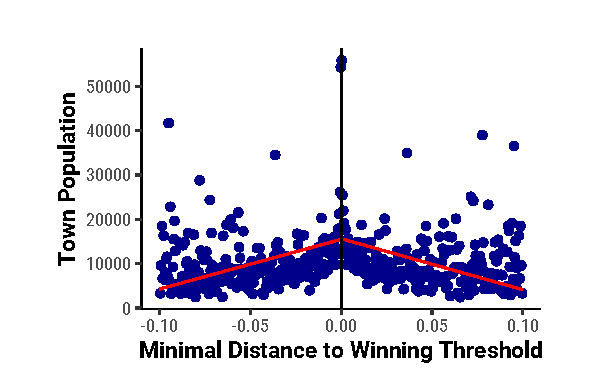
\includegraphics[width = 1 \textwidth]{../output/figures/norway_population.pdf}
        \caption{Municipality Population}
        \end{subfigure}%
        \begin{subfigure}[t]{0.48\textwidth}
        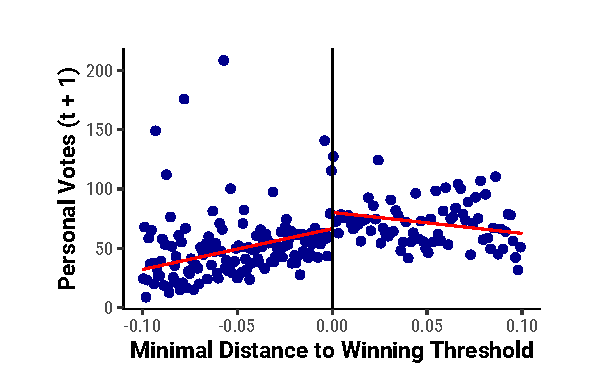
\includegraphics[width = 1 \textwidth]{../output/figures/norway_raw_pv.pdf}
        \caption{Raw Personal Votes (t + 1)}
        \end{subfigure}
    \caption{Distribution of Municipality Population size and Raw Personal Votes around Threshold}
    \label{app:norway_pv_plot1}
\end{figure}

\begin{figure}[htbp]
    \centering
    \begin{subfigure}[t]{0.48\textwidth}
        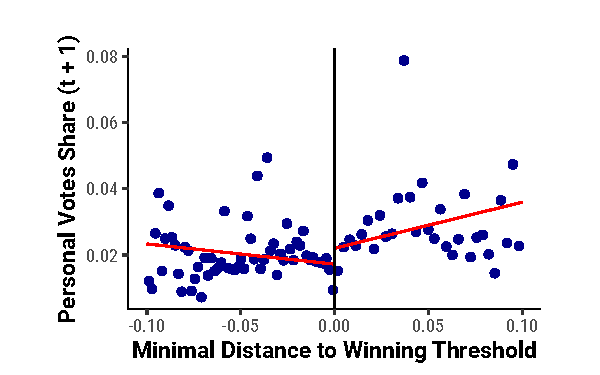
\includegraphics[width = 1 \textwidth]{../output/figures/norway_pv_share.pdf}
        \caption{Personal Vote / Total Votes (t + 1)}
        \end{subfigure}%
        \begin{subfigure}[t]{0.48\textwidth}
        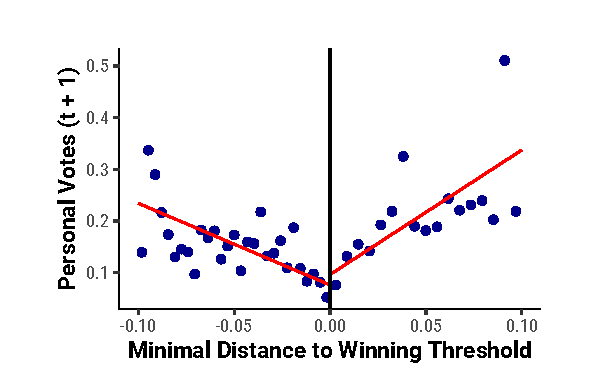
\includegraphics[width = 1 \textwidth]{../output/figures/norway_pv_share_p.pdf}
        \caption{Personal Vote / Party Votes (t + 1)}
        \end{subfigure}
    \caption{Distribution of Personal Vote Shares Around Threshold}
    \label{app:norway_pv_plot2}
\end{figure}


% \clearpage
% \subsubsection{Comparing Distribution of Personal Votes}

% As a simple check, we can plot the distribution of personal vote counts among barely elected candidates by candidate sex, and compare it to the distribution of personal votes in $t + 1$ among the same sample. Figure \ref{fig:pv_distribution} does exactly that. We see that at time $t$, the distribution of preference votes is almost exactly the same for either sex. When looking at the distribution of preference votes that these barely elected candidates received in the next election, we see that the distribution for men shifts slightly to the right compared to the one for women. This is further evidence that men receive a greater increase in personal votes as a result of being elected than female colleagues.

% \begin{figure}[htbp]
%     \centering
%     \begin{subfigure}[t]{0.48\textwidth}
%         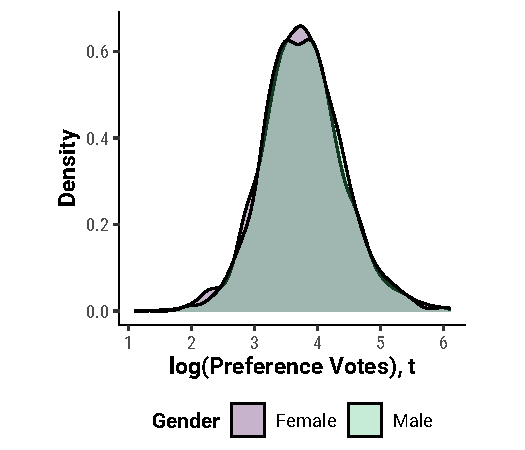
\includegraphics[width = 1 \textwidth]{../output/figures/pv_density_pre.pdf}
%         \caption{at $t$}
%         \end{subfigure}%
%         \begin{subfigure}[t]{0.48\textwidth}
%         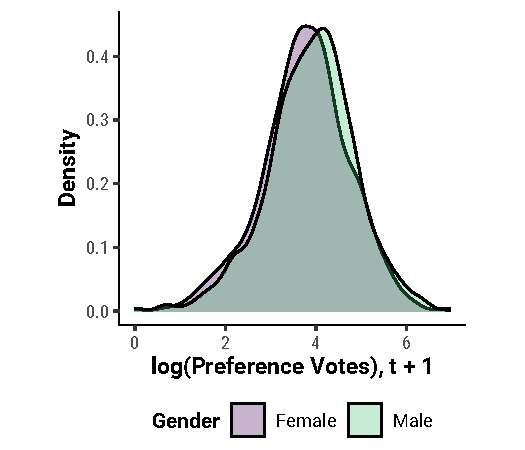
\includegraphics[width = 1 \textwidth]{../output/figures/pv_density_post.pdf}
%         \caption{at $t + 1$}
%         \end{subfigure}
%     \caption{Distribution of Personal Votes Among Borderline Elected}
%     \label{fig:pv_distribution}
% \end{figure}

\clearpage
\subsubsection{Robustness to Personal Vote Measurement}

Because of the aforementioned challenges, I estimate the heterogeneity-in-discontinuity specification with all the different outcome operationalisations discussed above. Table \ref{app:norway_pv_estimation} reports the results. The gender gap in the effect of incumbency on personal vote increases across right-wing parties persists across all specifications, although somewhat imprecisely estimated.

\begin{table}[!h]

\caption{\label{tab:norway_pv_check} \textbf{Sensitivity of Results to Different Personal Vote Measures.} The gender gap estimate is consistent across preferred measures.}
\centering
\fontsize{9}{11}\selectfont
\begin{threeparttable}
\begin{tabular}[t]{lcccccccc}
\toprule
\multicolumn{1}{c}{ } & \multicolumn{2}{c}{Raw PV} & \multicolumn{2}{c}{log(Raw PV)} & \multicolumn{2}{c}{PV / Total Votes} & \multicolumn{2}{c}{PV / Party Votes} \\
\cmidrule(l{3pt}r{3pt}){2-3} \cmidrule(l{3pt}r{3pt}){4-5} \cmidrule(l{3pt}r{3pt}){6-7} \cmidrule(l{3pt}r{3pt}){8-9}
  & \multicolumn{1}{c}{(1)} & \multicolumn{1}{c}{(2)} & \multicolumn{1}{c}{(3)} & \multicolumn{1}{c}{(4)} & \multicolumn{1}{c}{(5)} & \multicolumn{1}{c}{(6)} & \multicolumn{1}{c}{(7)} & \multicolumn{1}{c}{(8)}\\
\midrule
Elected & 13.842 & 23.573 & 0.243 & 0.340 & 0.003 & 0.005 & 0.012 & 0.031\\
 & (6.882) & (5.948) & (0.085) & (0.067) & (0.002) & (0.001) & (0.009) & (0.010)\\
\addlinespace
Female & -9.542 & 20.199 & -0.153 & -0.019 & -0.003 & 0.000 & 0.006 & 0.004\\
 & (8.383) & (27.847) & (0.100) & (0.101) & (0.003) & (0.002) & (0.008) & (0.011)\\
\addlinespace
Elected x Female & 12.549 & -34.571 & 0.095 & -0.229 & 0.001 & -0.005 & -0.009 & -0.024\\
 & (14.673) & (29.305) & (0.156) & (0.139) & (0.004) & (0.003) & (0.013) & (0.015)\\
\addlinespace \midrule \addlinespace
\addlinespace
Parties & \multicolumn{1}{c}{Left} & \multicolumn{1}{c}{Right} & \multicolumn{1}{c}{Left} & \multicolumn{1}{c}{Right} & \multicolumn{1}{c}{Left} & \multicolumn{1}{c}{Right} & \multicolumn{1}{c}{Left} & \multicolumn{1}{c}{Right}\\
Bandwidth & 0.067 & 0.093 & 0.05 & 0.073 & 0.025 & 0.052 & 0.013 & 0.046\\
Outcome Mean & 65.6 & 69.1 & 3.77 & 3.76 & 0.0204 & 0.0175 & 0.069 & 0.124\\
N (left) & \multicolumn{1}{c}{586} & \multicolumn{1}{c}{1019} & \multicolumn{1}{c}{553} & \multicolumn{1}{c}{941} & \multicolumn{1}{c}{446} & \multicolumn{1}{c}{840} & \multicolumn{1}{c}{352} & \multicolumn{1}{c}{791}\\
N (right) & \multicolumn{1}{c}{604} & \multicolumn{1}{c}{1048} & \multicolumn{1}{c}{564} & \multicolumn{1}{c}{962} & \multicolumn{1}{c}{458} & \multicolumn{1}{c}{856} & \multicolumn{1}{c}{358} & \multicolumn{1}{c}{803}\\
\bottomrule
\end{tabular}
\begin{tablenotes}[para]
\item All estimates are reported with robust standard errors clustered at the municipality level in parentheses. Each observation is a candidate's election attempt. 'Elected' is an indicator for observations where the candidate obtained a seat in the municipal council. 'Female' is an indicator for observations identified as female. `Elected` times `Female` is the interaction between the two variables. Other coefficients not reported. Regression run on all candidates in elections between 2003 and 2015.
\end{tablenotes}
\end{threeparttable}
\end{table}

\clearpage
\subsubsection{Robustness to Data Sample}
\label{app:norway_pv_data}

All analyses on personal vote outcomes so far were restricted to candidates in municipalities where all personal votes are recorded. This is important because we want our denominators for the shares to be right.  Still, for robustness's sake, I also report the estimates for the full sample in Table \ref{tab:norway_pv_check_no_drop}. Note that I can still extend the analyses to these additional observations because the personal vote measure(s) are not missing for the barely elected candidates -- they are merely missing for other (usually minor) candidates running in the municipality.

The estimates for raw personal vote and vote share (relative to total votes) remain consistent, and even gain some precision. The estimates for PV / Party Votes do change, however and are very noisy. This is, as mentioned before, likely due to the estimation challenge with this outcome in particular, where the results are sensitive to even a small degree of noise or measurement error.

\begin{table}[!h]

\caption{\label{tab:norway_pv_check_no_drop} \textbf{Sensitivity of Results to Different Personal Vote Measures.} Including Municipalities With Incomplete Personal Vote Data. }
\centering
\fontsize{9}{11}\selectfont
\begin{threeparttable}
\begin{tabular}[t]{lcccccccc}
\toprule
\multicolumn{1}{c}{ } & \multicolumn{2}{c}{Raw PV} & \multicolumn{2}{c}{log(Raw PV)} & \multicolumn{2}{c}{PV / Total Votes} & \multicolumn{2}{c}{PV / Party Votes} \\
\cmidrule(l{3pt}r{3pt}){2-3} \cmidrule(l{3pt}r{3pt}){4-5} \cmidrule(l{3pt}r{3pt}){6-7} \cmidrule(l{3pt}r{3pt}){8-9}
  & \multicolumn{1}{c}{(1)} & \multicolumn{1}{c}{(2)} & \multicolumn{1}{c}{(3)} & \multicolumn{1}{c}{(4)} & \multicolumn{1}{c}{(5)} & \multicolumn{1}{c}{(6)} & \multicolumn{1}{c}{(7)} & \multicolumn{1}{c}{(8)}\\
\midrule
Elected & 18.040 & 25.384 & 0.228 & 0.381 & 0.003 & 0.004 & 0.009 & 0.016\\
 & (6.289) & (4.625) & (0.068) & (0.056) & (0.002) & (0.001) & (0.007) & (0.009)\\
\addlinespace
Female & -3.911 & 16.047 & -0.098 & -0.018 & -0.002 & 0.001 & 0.004 & 0.012\\
 & (6.929) & (20.862) & (0.092) & (0.089) & (0.003) & (0.001) & (0.006) & (0.011)\\
\addlinespace
Elected x Female & 2.739 & -36.455 & 0.014 & -0.282 & 0.000 & -0.004 & -0.010 & -0.006\\
 & (11.299) & (22.658) & (0.133) & (0.127) & (0.003) & (0.002) & (0.011) & (0.014)\\
\addlinespace \midrule \addlinespace
\addlinespace
Parties & \multicolumn{1}{c}{Left} & \multicolumn{1}{c}{Right} & \multicolumn{1}{c}{Left} & \multicolumn{1}{c}{Right} & \multicolumn{1}{c}{Left} & \multicolumn{1}{c}{Right} & \multicolumn{1}{c}{Left} & \multicolumn{1}{c}{Right}\\
Bandwidth & 0.059 & 0.087 & 0.038 & 0.068 & 0.022 & 0.048 & 0.012 & 0.039\\
Outcome Mean & 60 & 64.8 & 3.69 & 3.66 & 0.0188 & 0.0168 & 0.0648 & 0.118\\
N (left) & \multicolumn{1}{c}{856} & \multicolumn{1}{c}{1457} & \multicolumn{1}{c}{769} & \multicolumn{1}{c}{1341} & \multicolumn{1}{c}{657} & \multicolumn{1}{c}{1166} & \multicolumn{1}{c}{519} & \multicolumn{1}{c}{1064}\\
N (right) & \multicolumn{1}{c}{861} & \multicolumn{1}{c}{1463} & \multicolumn{1}{c}{773} & \multicolumn{1}{c}{1343} & \multicolumn{1}{c}{663} & \multicolumn{1}{c}{1160} & \multicolumn{1}{c}{530} & \multicolumn{1}{c}{1068}\\
\bottomrule
\end{tabular}
\begin{tablenotes}[para]
\item All estimates are reported with robust standard errors clustered at the municipality level in parentheses. Each observation is a candidate's election attempt. 'Elected' is an indicator for observations where the candidate obtained a seat in the municipal council. 'Female' is an indicator for observations identified as female. `Elected` times `Female` is the interaction between the two variables. Other coefficients not reported. Regression run on all candidates in elections between 2003 and 2015.
\end{tablenotes}
\end{threeparttable}
\end{table}

\clearpage
\subsubsection{Robustness to Functional Form}

Finally, I also report estimates from specifications with second-order polynomials in Table \ref{tab:norway_pv_check_poly}. The results become a lot noisier; the general pattern of results, along with the estimates' sign and magnitude, still holds up for raw and logged personal vote counts. As discussed before, the specifications using share-based measures as an outcome are much more susceptible to noise -- especially with more demanding specifications such as second-order polynomials -- and should therefore be treated with caution.

\begin{table}[!h]

\caption{\label{tab:norway_pv_check_poly} \textbf{Sensitivity of Results to Different Personal Vote Measures, With Second-Order Polynomials.} The results become noisier, but remain consistent.}
\centering
\fontsize{9}{11}\selectfont
\begin{threeparttable}
\begin{tabular}[t]{lcccccccc}
\toprule
\multicolumn{1}{c}{ } & \multicolumn{2}{c}{Raw PV} & \multicolumn{2}{c}{log(Raw PV)} & \multicolumn{2}{c}{PV / Total Votes} & \multicolumn{2}{c}{PV / Party Votes} \\
\cmidrule(l{3pt}r{3pt}){2-3} \cmidrule(l{3pt}r{3pt}){4-5} \cmidrule(l{3pt}r{3pt}){6-7} \cmidrule(l{3pt}r{3pt}){8-9}
  & \multicolumn{1}{c}{(1)} & \multicolumn{1}{c}{(2)} & \multicolumn{1}{c}{(3)} & \multicolumn{1}{c}{(4)} & \multicolumn{1}{c}{(5)} & \multicolumn{1}{c}{(6)} & \multicolumn{1}{c}{(7)} & \multicolumn{1}{c}{(8)}\\
\midrule
Elected & 6.901 & 36.748 & 0.102 & 0.424 & 0.000 & 0.001 & 0.011 & 0.008\\
 & (9.262) & (7.169) & (0.107) & (0.090) & (0.003) & (0.003) & (0.009) & (0.012)\\
\addlinespace
Female & -11.687 & 33.684 & -0.126 & -0.002 & -0.001 & 0.000 & 0.005 & -0.006\\
 & (10.981) & (36.674) & (0.126) & (0.122) & (0.003) & (0.002) & (0.009) & (0.011)\\
\addlinespace
Elected x Female & 31.003 & -59.560 & 0.175 & -0.225 & 0.001 & 0.000 & -0.008 & -0.014\\
 & (20.053) & (37.342) & (0.204) & (0.182) & (0.004) & (0.004) & (0.014) & (0.018)\\
\addlinespace \midrule \addlinespace
\addlinespace
Parties & \multicolumn{1}{c}{Left} & \multicolumn{1}{c}{Right} & \multicolumn{1}{c}{Left} & \multicolumn{1}{c}{Right} & \multicolumn{1}{c}{Left} & \multicolumn{1}{c}{Right} & \multicolumn{1}{c}{Left} & \multicolumn{1}{c}{Right}\\
Bandwidth & 0.067 & 0.093 & 0.05 & 0.073 & 0.025 & 0.052 & 0.013 & 0.046\\
Outcome Mean & 65.6 & 69.1 & 3.77 & 3.76 & 0.0204 & 0.0175 & 0.069 & 0.124\\
N (left) & \multicolumn{1}{c}{586} & \multicolumn{1}{c}{1019} & \multicolumn{1}{c}{553} & \multicolumn{1}{c}{941} & \multicolumn{1}{c}{446} & \multicolumn{1}{c}{840} & \multicolumn{1}{c}{352} & \multicolumn{1}{c}{791}\\
N (right) & \multicolumn{1}{c}{604} & \multicolumn{1}{c}{1048} & \multicolumn{1}{c}{564} & \multicolumn{1}{c}{962} & \multicolumn{1}{c}{458} & \multicolumn{1}{c}{856} & \multicolumn{1}{c}{358} & \multicolumn{1}{c}{803}\\
\bottomrule
\end{tabular}
\begin{tablenotes}[para]
\item All estimates are reported with robust standard errors clustered at the municipality level in parentheses. Each observation is a candidate's election attempt. 'Elected' is an indicator for observations where the candidate obtained a seat in the municipal council. 'Female' is an indicator for observations identified as female. `Elected` times `Female` is the interaction between the two variables. Other coefficients not reported. Regression run on all candidates in elections between 2003 and 2015.
\end{tablenotes}
\end{threeparttable}
\end{table}

\clearpage
\subsection{Rank Position and Personal Votes}
\label{app:pv_by_rank}

Below, I plot the average number of personal votes by list rank, grouped by size of the council. We see that pre-vote rank ordering is a strong (though imperfect) predictor of the number of personal votes.

\begin{figure}[htbp]
    \centering
    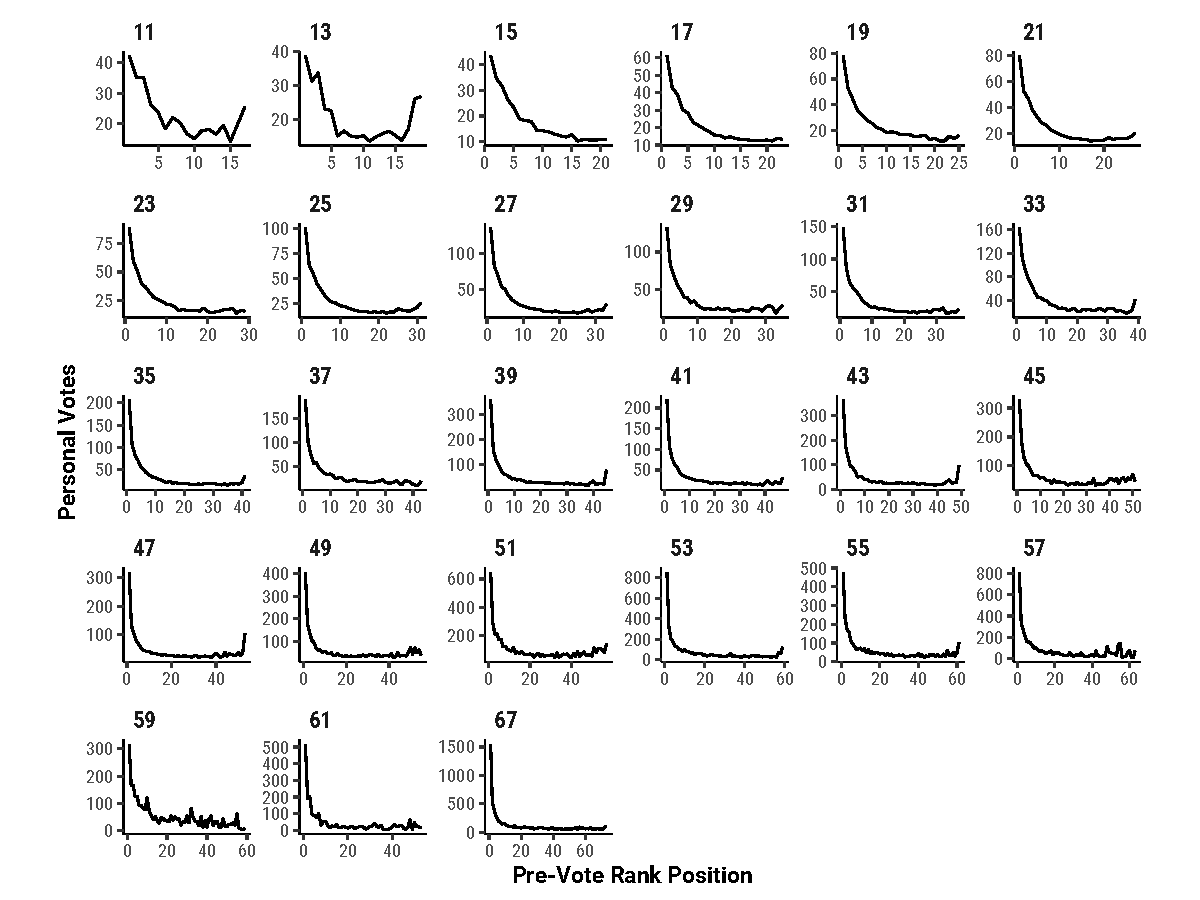
\includegraphics[width = .9\textwidth]{../output/figures/norway_pv_by_rank.pdf}
    \caption{Average number of personal votes, by list rank and council size.}
    \label{fig:pv_by_rank}
\end{figure}

\clearpage
\subsection{Differential Selection and Characteristics Correlated With Gender}
\label{app:age_rd}

Is the 'gender gap' specific to this characteristic, or do other candidate characteristics also moderate the incumbency advantage? Using the same difference-in-discontinuities specification as in the main results, I check whether there is a meaningful difference in incumbency effects between candidates below and above the median age. Unfortunately, due to data availability, I can only provide these estimates for Norway.

\begin{table}[!h]

\caption{\label{tab:norway_main_by_age} \textbf{Heterogeneity-in-Discontinuity Estimates For Incumbency Advantage In Norwegian Municipalities, By Age Group}. No Meaningful Difference Between Younger And Older Candidates.}
\centering
\fontsize{9}{11}\selectfont
\begin{threeparttable}
\begin{tabular}[t]{lS[
              input-symbols=(),
              table-format=-1.3,
              table-space-text-pre    = (,
              table-space-text-post   = ),
              input-open-uncertainty  =,
              input-close-uncertainty = ,
              table-align-text-post = false]S[
              input-symbols=(),
              table-format=-1.3,
              table-space-text-pre    = (,
              table-space-text-post   = ),
              input-open-uncertainty  =,
              input-close-uncertainty = ,
              table-align-text-post = false]S[
              input-symbols=(),
              table-format=-1.3,
              table-space-text-pre    = (,
              table-space-text-post   = ),
              input-open-uncertainty  =,
              input-close-uncertainty = ,
              table-align-text-post = false]S[
              input-symbols=(),
              table-format=-1.3,
              table-space-text-pre    = (,
              table-space-text-post   = ),
              input-open-uncertainty  =,
              input-close-uncertainty = ,
              table-align-text-post = false]S[
              input-symbols=(),
              table-format=-1.3,
              table-space-text-pre    = (,
              table-space-text-post   = ),
              input-open-uncertainty  =,
              input-close-uncertainty = ,
              table-align-text-post = false]S[
              input-symbols=(),
              table-format=-1.3,
              table-space-text-pre    = (,
              table-space-text-post   = ),
              input-open-uncertainty  =,
              input-close-uncertainty = ,
              table-align-text-post = false]}
\toprule
\multicolumn{1}{c}{ } & \multicolumn{3}{c}{Run (t + 1)} & \multicolumn{3}{c}{Win (t + 1)} \\
\cmidrule(l{3pt}r{3pt}){2-4} \cmidrule(l{3pt}r{3pt}){5-7}
  & \multicolumn{1}{c}{(1)} & \multicolumn{1}{c}{(2)} & \multicolumn{1}{c}{(3)} & \multicolumn{1}{c}{(4)} & \multicolumn{1}{c}{(5)} & \multicolumn{1}{c}{(6)}\\
\midrule
Elected & 0.007 & -0.002 & 0.013 & 0.076 & 0.075 & 0.064\\
 & (0.019) & (0.017) & (0.024) & (0.018) & (0.016) & (0.022)\\
\addlinespace
Age 48+ & 0.098 & 0.088 & 0.108 & -0.043 & -0.037 & -0.032\\
 & (0.020) & (0.018) & (0.024) & (0.015) & (0.014) & (0.019)\\
\addlinespace
Elected x Age 48+ & -0.012 & -0.002 & -0.023 & 0.013 & 0.018 & 0.012\\
 & (0.029) & (0.026) & (0.036) & (0.025) & (0.022) & (0.030)\\
\addlinespace \midrule \addlinespace
Bandwidth & 0.054 & 0.11 & 0.027 & 0.05 & 0.099 & 0.025\\
BW Type & \multicolumn{1}{c}{Optimal} & \multicolumn{1}{c}{2x Opt} & \multicolumn{1}{c}{0.5x Opt} & \multicolumn{1}{c}{Optimal} & \multicolumn{1}{c}{2x Opt} & \multicolumn{1}{c}{0.5x Opt}\\
Outcome Mean & 0.564 & 0.575 & 0.551 & 0.261 & 0.263 & 0.257\\
N (left) & \multicolumn{1}{c}{4617} & \multicolumn{1}{c}{5529} & \multicolumn{1}{c}{3667} & \multicolumn{1}{c}{4502} & \multicolumn{1}{c}{5428} & \multicolumn{1}{c}{3549}\\
N (right) & \multicolumn{1}{c}{4666} & \multicolumn{1}{c}{5590} & \multicolumn{1}{c}{3711} & \multicolumn{1}{c}{4551} & \multicolumn{1}{c}{5489} & \multicolumn{1}{c}{3592}\\
\bottomrule
\end{tabular}
\begin{tablenotes}[para]
\item All estimates are reported with robust standard errors clustered at the municipality level in parentheses. Each observation is a candidate's election attempt. 'Elected' is an indicator for observations where the candidate obtained a seat in the municipal council. 'Age 48+' is an indicator for candidates older than 47 at the time of the election. `Elected` times `Female` is the interaction between the two variables. Other coefficients not reported. Regression run on all candidates in elections between 2003 and 2015.
\end{tablenotes}
\end{threeparttable}
\end{table}

The results offer no evidence of any age-based gap in incumbency advantages.

Next, I also code candidates on whether they have run as candidate before or not. I use this binary 'experience' variable as an additional moderator for my heterogeneity-in-discontinuity design. As with age, I find no significant differential effect in the incumbency effect based on experience.

\begin{table}[!h]

\caption{\label{tab:norway_by_experience} \textbf{Difference-in-Discontinuity Estimates For Incumbency Advantage In Norwegian Municipalities, By Political Experience.} No Difference Between First-Time And Multiple-Time Candidates.}
\centering
\fontsize{9}{11}\selectfont
\begin{threeparttable}
\begin{tabular}[t]{lS[
              input-symbols=(),
              table-format=-1.3,
              table-space-text-pre    = (,
              table-space-text-post   = ),
              input-open-uncertainty  =,
              input-close-uncertainty = ,
              table-align-text-post = false]S[
              input-symbols=(),
              table-format=-1.3,
              table-space-text-pre    = (,
              table-space-text-post   = ),
              input-open-uncertainty  =,
              input-close-uncertainty = ,
              table-align-text-post = false]S[
              input-symbols=(),
              table-format=-1.3,
              table-space-text-pre    = (,
              table-space-text-post   = ),
              input-open-uncertainty  =,
              input-close-uncertainty = ,
              table-align-text-post = false]S[
              input-symbols=(),
              table-format=-1.3,
              table-space-text-pre    = (,
              table-space-text-post   = ),
              input-open-uncertainty  =,
              input-close-uncertainty = ,
              table-align-text-post = false]S[
              input-symbols=(),
              table-format=-1.3,
              table-space-text-pre    = (,
              table-space-text-post   = ),
              input-open-uncertainty  =,
              input-close-uncertainty = ,
              table-align-text-post = false]S[
              input-symbols=(),
              table-format=-1.3,
              table-space-text-pre    = (,
              table-space-text-post   = ),
              input-open-uncertainty  =,
              input-close-uncertainty = ,
              table-align-text-post = false]}
\toprule
\multicolumn{1}{c}{ } & \multicolumn{3}{c}{Run (t + 1)} & \multicolumn{3}{c}{Win (t + 1)} \\
\cmidrule(l{3pt}r{3pt}){2-4} \cmidrule(l{3pt}r{3pt}){5-7}
  & \multicolumn{1}{c}{(1)} & \multicolumn{1}{c}{(2)} & \multicolumn{1}{c}{(3)} & \multicolumn{1}{c}{(4)} & \multicolumn{1}{c}{(5)} & \multicolumn{1}{c}{(6)}\\
\midrule
Elected & -0.010 & -0.001 & -0.009 & 0.083 & 0.093 & 0.069\\
 & (0.019) & (0.016) & (0.023) & (0.017) & (0.015) & (0.021)\\
\addlinespace
Experience & 0.050 & 0.074 & 0.044 & -0.026 & -0.013 & -0.025\\
 & (0.020) & (0.017) & (0.026) & (0.017) & (0.015) & (0.021)\\
\addlinespace
Elected x Experience & 0.027 & -0.003 & 0.032 & -0.005 & -0.025 & 0.002\\
 & (0.032) & (0.026) & (0.040) & (0.026) & (0.022) & (0.032)\\
\addlinespace \midrule \addlinespace
Bandwidth & 0.054 & 0.11 & 0.027 & 0.05 & 0.099 & 0.025\\
BW Type & \multicolumn{1}{c}{Optimal} & \multicolumn{1}{c}{2x Opt} & \multicolumn{1}{c}{0.5x Opt} & \multicolumn{1}{c}{Optimal} & \multicolumn{1}{c}{2x Opt} & \multicolumn{1}{c}{0.5x Opt}\\
Outcome Mean & 0.564 & 0.575 & 0.551 & 0.261 & 0.263 & 0.257\\
N (left) & \multicolumn{1}{c}{4617} & \multicolumn{1}{c}{5529} & \multicolumn{1}{c}{3667} & \multicolumn{1}{c}{4502} & \multicolumn{1}{c}{5428} & \multicolumn{1}{c}{3549}\\
N (right) & \multicolumn{1}{c}{4666} & \multicolumn{1}{c}{5590} & \multicolumn{1}{c}{3711} & \multicolumn{1}{c}{4551} & \multicolumn{1}{c}{5489} & \multicolumn{1}{c}{3592}\\
\bottomrule
\end{tabular}
\begin{tablenotes}[para]
\item All estimates are reported with robust standard errors clustered at the municipality level in parentheses. Each observation is a candidate's election attempt. 'Elected' is an indicator for observations where the candidate obtained a seat in the municipal council. 'Female' is an indicator for observations identified as female. `Elected` times `Female` is the interaction between the two variables. Other coefficients not reported. Regression run on all candidates in elections between 2003 and 2015.
\end{tablenotes}
\end{threeparttable}
\end{table}

\clearpage
\subsection{Matching Estimates}
\label{app:matching}

In order to further reduce concerns about differential selection, I want to find the closest possible comparison group to female candidates in the threshold sample. To do so, I match observations on a number of dimensions: candidates' age, experience, the year of the election, their party and the province / county in which they run. I describe the matching procedure in greater detail and report the results below in Table \ref{tab:norway_match}. Importantly, even in the strictest setting -- matching the closest male threshold candidate in terms of age, experience and election year in exactly the same party and county -- my estimates report a meaningful gender gap in the incumbency advantage (albeit with somewhat larger uncertainty).

\paragraph*{Matching Procedure.} For all matching estimates, I retain the set of female threshold candidates within the bandwidth of 0.05 and attempt to find the closest possible male candidate within the same bandwidth that matches this observation. Unlike in the original setting, I cannot rely on automatic bandwidth selection procedures, since the choice of bandwidth also affects the choice of matching pairs (that is, selecting $h$ on the full sample may no longer be MSE-optimal after only retaining matches within $h$).

Throughout, I match without replacement. First, I use simple distance-based (Mahalnobis) matching to find the closest male candidate in terms of running variable, age, experience, and election year (columns 1 and 2). I then restrict possible matches to those within exactly the same party (column 3) and exactly the same province (column 4). Finally, I pick the male candidate with the closest election margin, age, experience and election year who runs in both the same party as well as the same province (column 5).

\paragraph*{Results.} The results suggest that even when comparing the incumbency advantage among men and women with similar profiles, and from the same party and geography, there is a notable gender gap, decreasing the incumbency advantage for women by more than 50\% on average. That said, it is worth emphasising that the matching estimates in columns (4) and (5) are somewhat reduced in magnitude and no longer statistically significant at the conventional significance level of .05. While these estimates reduce the concern that differential selection or candidate attributes other than, yet correlated with gender can explain the contrast in incumbency advantages, a remaining caveat is that my list of candidate covariates is finite and non-exhaustive.

\begin{table}[!h]

\caption{\label{tab:norway_match} \textbf{Matched Estimates.}}
\centering
\fontsize{9}{11}\selectfont
\begin{threeparttable}
\begin{tabular}[t]{lS[
              input-symbols=(),
              table-format=-1.3,
              table-space-text-pre    = (,
              table-space-text-post   = ),
              input-open-uncertainty  =,
              input-close-uncertainty = ,
              table-align-text-post = false]S[
              input-symbols=(),
              table-format=-1.3,
              table-space-text-pre    = (,
              table-space-text-post   = ),
              input-open-uncertainty  =,
              input-close-uncertainty = ,
              table-align-text-post = false]S[
              input-symbols=(),
              table-format=-1.3,
              table-space-text-pre    = (,
              table-space-text-post   = ),
              input-open-uncertainty  =,
              input-close-uncertainty = ,
              table-align-text-post = false]S[
              input-symbols=(),
              table-format=-1.3,
              table-space-text-pre    = (,
              table-space-text-post   = ),
              input-open-uncertainty  =,
              input-close-uncertainty = ,
              table-align-text-post = false]S[
              input-symbols=(),
              table-format=-1.3,
              table-space-text-pre    = (,
              table-space-text-post   = ),
              input-open-uncertainty  =,
              input-close-uncertainty = ,
              table-align-text-post = false]}
\toprule
\multicolumn{1}{c}{ } & \multicolumn{5}{c}{Win (t + 1)} \\
\cmidrule(l{3pt}r{3pt}){2-6}
  & \multicolumn{1}{c}{(1)} & \multicolumn{1}{c}{(2)} & \multicolumn{1}{c}{(3)} & \multicolumn{1}{c}{(4)} & \multicolumn{1}{c}{(5)}\\
\midrule
Elected & 0.104 & 0.107 & 0.113 & 0.081 & 0.086\\
 & (0.020) & (0.021) & (0.020) & (0.021) & (0.022)\\
\addlinespace
Female & -0.033 & -0.033 & -0.041 & -0.046 & -0.044\\
 & (0.019) & (0.019) & (0.019) & (0.019) & (0.020)\\
\addlinespace
Elected x Female & -0.062 & -0.065 & -0.073 & -0.039 & -0.046\\
 & (0.029) & (0.030) & (0.029) & (0.029) & (0.031)\\
\addlinespace \midrule \addlinespace
Bandwidth & 0.05 & 0.05 & 0.05 & 0.05 & 0.05\\
N & 7128 & 7128 & 7068 & 7128 & 6804\\
Individual Match & Y & Y & Y & Y & Y\\
Year Match & Y &  & Y & Y & Y\\
Year (Factor) Match &  & Y &  &  & \\
Party Match &  &  & Y &  & Y\\
Province Match &  &  &  & Y & Y\\
\bottomrule
\end{tabular}
\begin{tablenotes}[para]
\item All estimates are reported with robust standard errors clustered at the municipality level in parentheses. 'Individual Match' indicates 1:1 distance-based matching on age and experience; 'Year' match indicates 1:1 distance-based matching on election year; 'Year (Factor)' treats election year as a dummy variable; 'Party Match' and 'Province Match' indicates 1:1 exact matching on party and province, respectively.
\end{tablenotes}
\end{threeparttable}
\end{table}

\clearpage
\subsection{Heterogeneity By Population Size}
\label{app:hetero_norway}

In this section, I examine whether cities that are outliers in terms of population drive my results. Although the gender gap is concentrated among cities in the upper tercile (consistent with the name recognition mechanism), I find no evidence that the overall result is sensitive to excluding the largest cities.

\subsubsection{Sensitivity to Outliers}
\label{app:norway_outliers}

My estimates hold up even when restricting the sample to towns below a population of 20,000. When restricting the sample to towns smaller than 10,000 population, the effect of winning on winning again moves towards zero, but remains negative. In line with Appendix \ref{app:effects_by_tercile}, I interpret this as evidence for name recognition mechanisms in larger municipalities driving the effect.

\begin{figure}[!htb]
    \centering
    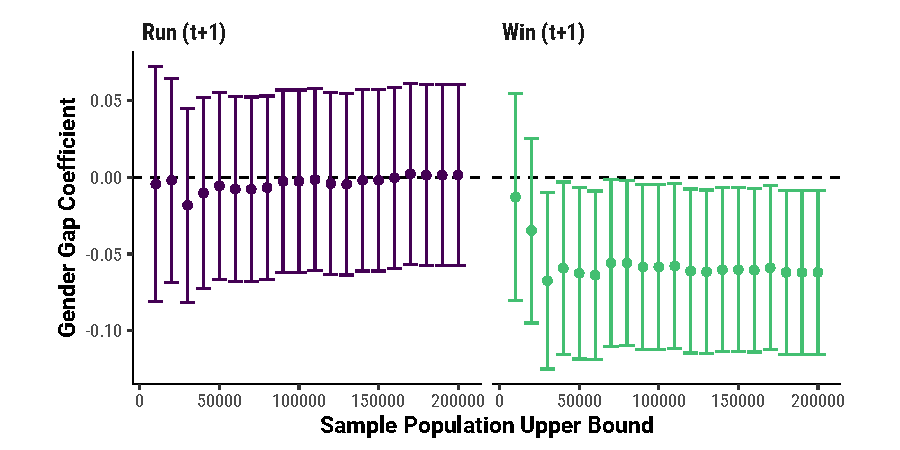
\includegraphics[width = 0.8 \textwidth]{../output/figures/norway_muni_robust.pdf}
    \caption{\textbf{Gender Gap in Incumbency Effect, Norway, By Maximum Municipality Size Included.}}
    \label{fig:norway_outliers}
\end{figure}



\clearpage
\subsubsection{Effect Magnitude by Population Tercile}
\label{app:effects_by_tercile}

Next I also estimate the gender gap on subsamples binned by population tercile. The results suggest that the negative effect in the Norwegian case is primarily driven by the upper tercile, i.e. the largest municipalities (but, as the previous appendix section suggests, not just its extreme outliers). This finding is consistent with the argument that name recognition is a key driver of personal vote incumbency advantages in Norway: in smaller municipalities (with shorter lists and fewer candidates), voters may know the handful of elected female candidates better.


\begin{figure}[!htb]
    \centering
    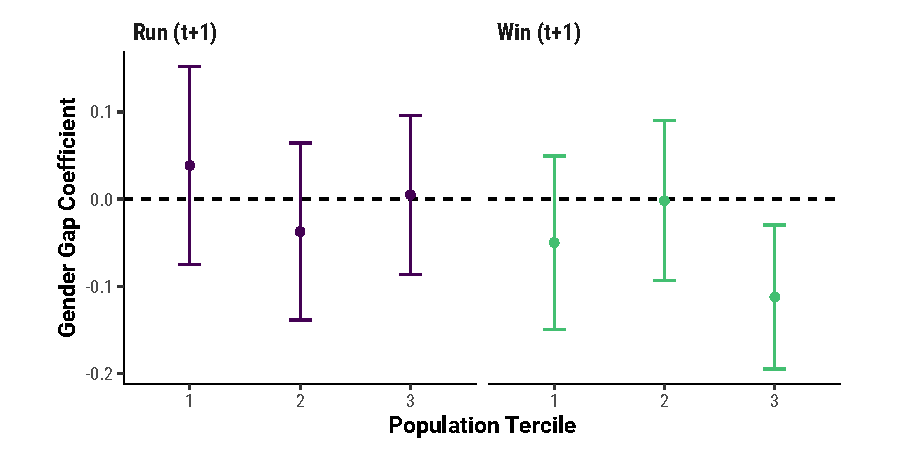
\includegraphics[width = 0.8 \textwidth]{../output/figures/norway_tercile_robust.pdf}
    \caption{\textbf{Gender Gap in Incumbency Effect, Norway, By Population Tercile.}}
    \label{fig:norway_tercile_robust}
\end{figure}



\clearpage
\subsection{Survey Evidence On Voters' Attitudes Towards Female Candidates}
\label{app:norway_survey}

Next, I examine data from the 2015 Local Election Survey in Norway (conducted by the University of Oslo) to test whether right-wing voters hold more negative views about women in politics. I plot the share of respondents from each party agreeing that ``Women should play a \emph{greater} role in local [municipal] politics.'' The sample analysed included 882 respondents. A majority of respondents in left-leaning parties agrees with this statement, whereas the share of respondents agreeing in right-wing parties hovers around 40\%.

\begin{figure}[!htb]
    \centering
    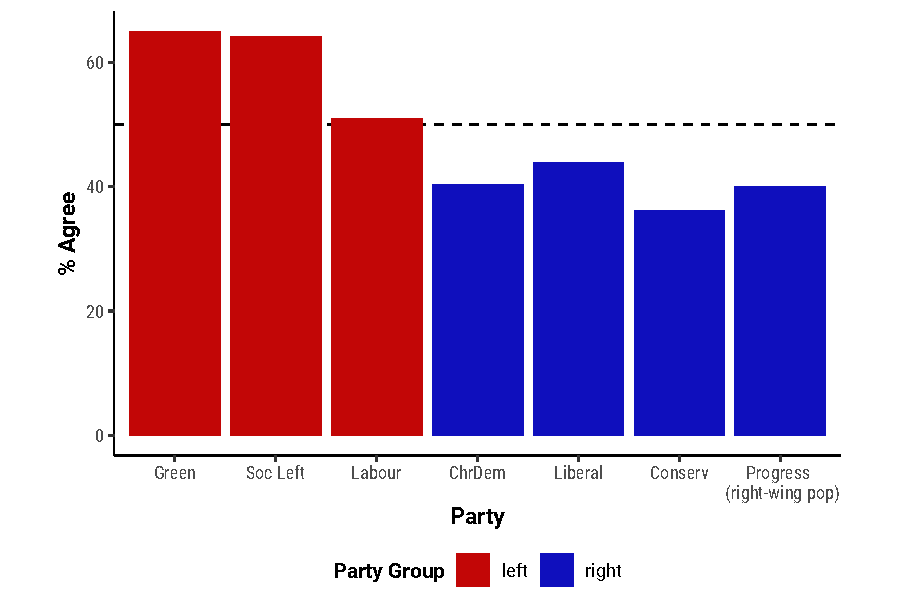
\includegraphics[width = 1 \textwidth]{../output/figures/norway_survey_support.pdf}
    \caption{\textbf{Share Respondents Agreeing That Women Should Play Greater Role In Local Politics, By Party.}}
    \label{fig:norway_survey}
\end{figure}



% \subsection{Testing For Heterogeneity Across Population Sizes}
% \label{app:hetero}

% \subsection{Do Large Cities Drive The Result?}

% In this appendix, I investigate whether the estimated magnitude of the gender gap changes when I restrict my sample size to municipalities of a smaller size. Below, I plot the gender gap coefficients on my two primary outcomes for samples including all (borderline) candidates from municipalities with a population below $x$. In other words, to the right of the $x$-axis, the coefficient is estimated on a sample that includes larger municipalities.


\clearpage
\section{Additional Statistical Results: Spain}

\subsection{Estimates from Difference-in-Differences Specification}
\label{app:spain_did}

The large number of observations in the Spanish case allows me to compare the outcome mean of candidates extremely close to the threshold without making additional functional form assumptions. To do so, I estimate regressions of the form

\begin{equation}
    y_{it} = D_{it} + F_{i} + D_{it} \times F_{i} + \phi_{it}(\cdot) + \varepsilon_{it}
\end{equation}

on all observations within 1 (0.5, 0.25) percentage point(s) of the election margin. $D_{it}$ is a binary indicator whether the candidate $i$ in election $t$ was elected, and $F_i$ is a binary indicator for whether the candidate is recorded as female. As before, I include province and party-by-year fixed effects. The results, in Table \ref{tab:spain_did}, yield estimates that are consistent with those obtained using the heterogeneity-in-discontinuity approach.


\begin{table}[!h]

\caption{\label{tab:spain_did}. Estimates from Difference-in-Differences in Spanish Close Elections.}
\centering
\fontsize{9}{11}\selectfont
\begin{threeparttable}
\begin{tabular}[t]{lS[
              input-symbols=(),
              table-format=-1.3,
              table-space-text-pre    = (,
              table-space-text-post   = ),
              input-open-uncertainty  =,
              input-close-uncertainty = ,
              table-align-text-post = false]S[
              input-symbols=(),
              table-format=-1.3,
              table-space-text-pre    = (,
              table-space-text-post   = ),
              input-open-uncertainty  =,
              input-close-uncertainty = ,
              table-align-text-post = false]S[
              input-symbols=(),
              table-format=-1.3,
              table-space-text-pre    = (,
              table-space-text-post   = ),
              input-open-uncertainty  =,
              input-close-uncertainty = ,
              table-align-text-post = false]S[
              input-symbols=(),
              table-format=-1.3,
              table-space-text-pre    = (,
              table-space-text-post   = ),
              input-open-uncertainty  =,
              input-close-uncertainty = ,
              table-align-text-post = false]S[
              input-symbols=(),
              table-format=-1.3,
              table-space-text-pre    = (,
              table-space-text-post   = ),
              input-open-uncertainty  =,
              input-close-uncertainty = ,
              table-align-text-post = false]S[
              input-symbols=(),
              table-format=-1.3,
              table-space-text-pre    = (,
              table-space-text-post   = ),
              input-open-uncertainty  =,
              input-close-uncertainty = ,
              table-align-text-post = false]}
\toprule
\multicolumn{1}{c}{ } & \multicolumn{3}{c}{Run Again} & \multicolumn{3}{c}{Win Again} \\
\cmidrule(l{3pt}r{3pt}){2-4} \cmidrule(l{3pt}r{3pt}){5-7}
  & \multicolumn{1}{c}{(1)} & \multicolumn{1}{c}{(2)} & \multicolumn{1}{c}{(3)} & \multicolumn{1}{c}{(4)} & \multicolumn{1}{c}{(5)} & \multicolumn{1}{c}{(6)}\\
\midrule
Elected & 0.131 & 0.115 & 0.104 & 0.099 & 0.071 & 0.094\\
 & (0.014) & (0.019) & (0.028) & (0.012) & (0.017) & (0.025)\\
\addlinespace
Female & -0.022 & 0.002 & 0.021 & -0.016 & -0.029 & -0.015\\
 & (0.016) & (0.023) & (0.033) & (0.013) & (0.019) & (0.026)\\
\addlinespace
Elected x Female & 0.031 & 0.004 & -0.003 & 0.041 & 0.048 & 0.027\\
 & (0.023) & (0.032) & (0.047) & (0.020) & (0.029) & (0.041)\\
\addlinespace \midrule \addlinespace
Bandwidth & 0.01 & 0.005 & 0.0025 & 0.01 & 0.005 & 0.0025\\
Mean Out & 0.49 & 0.49 & 0.49 & 0.25 & 0.25 & 0.25\\
Avg No. votes & 26.17 & 13.4 & 6.82 & 26.17 & 13.4 & 6.82\\
\bottomrule
\end{tabular}
\begin{tablenotes}
\small
\item \textit{Note: } 
\item All estimates are reported with robust standard errors clustered at the municipality level in parentheses. Each observation is a candidate's election attempt. 'Elected' is an indicator for observations where the candidate obtained a seat in the municipal council. 'Female' is an indicator for observations identified as female. Bandwidth indicates the range of running variable margins included in the estimation. Avg. \# Votes is the average number of votes between the extreme end of the selected bandwidth and the election threshold.
\end{tablenotes}
\end{threeparttable}
\end{table}


\clearpage

\subsection{Heterogeneity Across Parties}
\label{app:spain_by_party}

In this section, I report the estimates from the main specification on different subgroups of the Spanish data. If the estimates fitted on left- and right-wing parties differ, the overall gender gap estimate in the main part of the manuscript might mask some important heterogeneities.

First, I fit the main specification on samples from left- and right-wing parties (PSOE and PP) separately. Table \ref{app:spain_by_party} reports the results with running and winning in the next election as outcomes.

There is a notable difference in the gender gap in the effect on running again: female candidates in left-wing parties experience a much smaller increase (relative to men) in their probability of running again in left-wing parties, compared to the same difference in right-wing parties. However, the estimate is also somewhat imprecise.

More importantly, we see little difference in the gender gap in the incumbency effect on winning again between the two party samples. This suggests that there is no party-specific mechanism that drives results (and is consistent with an ideology-agnostic seniority norm), and that would be masked by pooling the sample.

\begin{table}[!h]

\caption{\label{tab:spain_by_party} \textbf{Difference-in-Discontinuity Estimates For Incumbency Advantage In Spanish Municipalities, By Political Party Group.} The estimates for the gender gap are similar in both left- and right-wing parties.}
\centering
\fontsize{9}{11}\selectfont
\begin{threeparttable}
\begin{tabular}[t]{lS[
              input-symbols=(),
              table-format=-1.3,
              table-space-text-pre    = (,
              table-space-text-post   = ),
              input-open-uncertainty  =,
              input-close-uncertainty = ,
              table-align-text-post = false]S[
              input-symbols=(),
              table-format=-1.3,
              table-space-text-pre    = (,
              table-space-text-post   = ),
              input-open-uncertainty  =,
              input-close-uncertainty = ,
              table-align-text-post = false]S[
              input-symbols=(),
              table-format=-1.3,
              table-space-text-pre    = (,
              table-space-text-post   = ),
              input-open-uncertainty  =,
              input-close-uncertainty = ,
              table-align-text-post = false]S[
              input-symbols=(),
              table-format=-1.3,
              table-space-text-pre    = (,
              table-space-text-post   = ),
              input-open-uncertainty  =,
              input-close-uncertainty = ,
              table-align-text-post = false]}
\toprule
\multicolumn{1}{c}{ } & \multicolumn{2}{c}{Run (t + 1)} & \multicolumn{2}{c}{Win (t + 1)} \\
\cmidrule(l{3pt}r{3pt}){2-3} \cmidrule(l{3pt}r{3pt}){4-5}
  & \multicolumn{1}{c}{(1)} & \multicolumn{1}{c}{(2)} & \multicolumn{1}{c}{(3)} & \multicolumn{1}{c}{(4)}\\
\midrule
Elected & 0.091 & 0.117 & 0.072 & 0.088\\
 & (0.024) & (0.023) & (0.020) & (0.021)\\
\addlinespace
Female & -0.029 & -0.009 & -0.011 & -0.041\\
 & (0.025) & (0.027) & (0.021) & (0.022)\\
\addlinespace
Elected x Female & 0.072 & 0.004 & 0.044 & 0.058\\
 & (0.036) & (0.039) & (0.031) & (0.034)\\
\addlinespace \midrule \addlinespace
Parties & \multicolumn{1}{c}{Left} & \multicolumn{1}{c}{Right} & \multicolumn{1}{c}{Left} & \multicolumn{1}{c}{Right}\\
Bandwidth & 0.029 & 0.032 & 0.032 & 0.03\\
Outcome Mean & 0.478 & 0.484 & 0.259 & 0.26\\
N (left) & \multicolumn{1}{c}{5663} & \multicolumn{1}{c}{5454} & \multicolumn{1}{c}{6134} & \multicolumn{1}{c}{5149}\\
N (right) & \multicolumn{1}{c}{5511} & \multicolumn{1}{c}{5433} & \multicolumn{1}{c}{5977} & \multicolumn{1}{c}{5130}\\
\bottomrule
\end{tabular}
\begin{tablenotes}[para]
\item All estimates are reported with robust standard errors clustered at the municipality level in parentheses. Each observation is a candidate's election attempt. 'Elected' is an indicator for observations where the candidate obtained a seat in the municipal council. 'Female' is an indicator for observations identified as female. `Elected` times `Female` is the interaction between the two variables. Other coefficients not reported. Regression run on all candidates in elections between 2003 and 2015.
\end{tablenotes}
\end{threeparttable}
\end{table}


\clearpage
\subsection{Heterogeneity Across Quota Rules}
\label{app:spain_by_quota}

Another worry is that estimating the average pooled over all municipalities masks some important heterogeneity across towns. In 2007, a gender quota started to apply to places with a population of above 5,000: lists in municipalities above this threshold must now feature at least 40\% of candidates from either gender. The requirement was extended to all municipalities above 3,000 pop. in 2011.

In the first subsection (\ref{app:below_quota}), I fit my heterogeneity-in-discontinuity design on municipalities with fewer than 3,000 population only. I continue to find that women's incumbency advantages are no smaller than men's in this subsample of municipalities without a quota.

Of course, these municipalities could be meaningfully different from larger ones where the quota did come into effect.

Ideally, to check whether the mandated quota drives these results, I would run a two-dimensional regression discontinuity with margin of victory and population size as independent assignment variables. This would allow me to check whether the estimates in Equation 2 meaningfully change at the threshold. Unfortunately, even with the amount of data from Spanish municipalities, such a design would be underpowered and consequently suffer from high uncertainty and noisy estimates.

Instead, I report additional results from two types of specifications. First, I fit the typical heterogeneity-in-discontinuity specification on either side of the municipality size threshold (\ref{app:diff-in-disc-quota}). The results offer no clear interpretation because of large uncertainty that comes with these estimates. In addition, I also offer estimates from a difference-in-difference strategy (\ref{app:diff-in-diff-quota}). While less clearly identified, these estimates come with lower variance. Together, I find no strong evidence that the legal gender quota in small municipalities is responsible for the lack of a gender gap in political careers in Spain.

\clearpage
\subsubsection{Municipalities without Gender Quota Alone}
\label{app:below_quota}

In this subsection, I report estimates from the Spanish sample of municipalities that never experienced a legally binding quota. We observe that even without a quota, women's incumbency advantages are larger than men's (estimated at an optimal bandwidth).

\begin{table}[!h]

\caption{\label{tab:spain_by_quota_below} Gender Gap in Incumbency Advantages, Spain, Non-Quota Municipalities (< 3,000 pop).}
\centering
\fontsize{8}{10}\selectfont
\begin{tabular}[t]{lS[
              input-symbols=(),
              table-format=-2.3,
              table-space-text-pre    = (,
              table-space-text-post   = ),
              input-open-uncertainty  =,
              input-close-uncertainty = ,
              table-align-text-post = false]S[
              input-symbols=(),
              table-format=-2.3,
              table-space-text-pre    = (,
              table-space-text-post   = ),
              input-open-uncertainty  =,
              input-close-uncertainty = ,
              table-align-text-post = false]}
\toprule
\multicolumn{1}{c}{ } & \multicolumn{1}{c}{Run (t+1)} & \multicolumn{1}{c}{Win (t+1)} \\
\cmidrule(l{3pt}r{3pt}){2-2} \cmidrule(l{3pt}r{3pt}){3-3}
  & \multicolumn{1}{c}{(1)} & \multicolumn{1}{c}{(2)}\\
\midrule
Elected & 0.111 & 0.033\\
 & (0.020) & (0.021)\\
Female & -0.024 & -0.040\\
 & (0.025) & (0.024)\\
Elected x Female & 0.044 & 0.097\\
 & (0.035) & (0.037)\\
\addlinespace \midrule \addlinespace
Bandwidth & 0.035 & 0.025\\
Outcome Mean & 0.471 & 0.239\\
N (left) & \multicolumn{1}{c}{7317} & \multicolumn{1}{c}{5209}\\
N (right) & \multicolumn{1}{c}{7489} & \multicolumn{1}{c}{5337}\\
\bottomrule
\end{tabular}
\end{table}

\clearpage
\subsubsection{Heterogeneity-in-Discontinuity Estimates}
\label{app:diff-in-disc-quota}

Following the introduction of the 3,000 pop. threshold in 2011, I compare candidates in municipalities between 250 and 3,000 population to candidates in municipalities between 3,001 and 6,000 population.\footnote{I exclude candidates from municipalities that cross the population threshold in between elections in this sample. The choice of bandwidth in this exercise is such that I have enough power to say something meaningful. Estimates that restrict the bandwidth to a narrower slice to municipalities around the 3,000 threshold end up being extremely noisy.} The approach assumes that municipalities within the bandwidth are comparable to one another, and any difference between the samples is driven by the quota alone. That said, the results are also noisier because I have to restrict my sample to post-2007 (i.e., post-quota introduction) observations.

Unsurprisingly, the estimates obtained from the heterogeneity-in-discontinuity specification come with a high degree of uncertainty: there simply are not that many observations close to the municipality threshold \emph{and} the electoral threshold. For each of the two outcomes, the estimates of the gender gap change signs across the two municipality samples (although in different directions). At the same time, the confidence intervals for these estimates also firmly includes null and the respective other point estimate. These results therefore offer little evidence that would suggest that the quota plays an important role in attenuating the gender gap.

\begin{table}[!h]

\caption{\label{tab:spain_by_quota} \textbf{Difference-in-Discontinuity Estimates For Incumbency Advantage In Spanish Municipalities, By Quota Law.} The estimates for the gender gap are similar in municipalities with and without the gender quota on lists.}
\centering
\fontsize{9}{11}\selectfont
\begin{threeparttable}
\begin{tabular}[t]{lS[
              input-symbols=(),
              table-format=-2.3,
              table-space-text-pre    = (,
              table-space-text-post   = ),
              input-open-uncertainty  =,
              input-close-uncertainty = ,
              table-align-text-post = false]S[
              input-symbols=(),
              table-format=-2.3,
              table-space-text-pre    = (,
              table-space-text-post   = ),
              input-open-uncertainty  =,
              input-close-uncertainty = ,
              table-align-text-post = false]S[
              input-symbols=(),
              table-format=-2.3,
              table-space-text-pre    = (,
              table-space-text-post   = ),
              input-open-uncertainty  =,
              input-close-uncertainty = ,
              table-align-text-post = false]S[
              input-symbols=(),
              table-format=-2.3,
              table-space-text-pre    = (,
              table-space-text-post   = ),
              input-open-uncertainty  =,
              input-close-uncertainty = ,
              table-align-text-post = false]}
\toprule
\multicolumn{1}{c}{ } & \multicolumn{2}{c}{Run (t+1)} & \multicolumn{2}{c}{Win (t+1)} \\
\cmidrule(l{3pt}r{3pt}){2-3} \cmidrule(l{3pt}r{3pt}){4-5}
  & \multicolumn{1}{c}{(1)} & \multicolumn{1}{c}{(2)} & \multicolumn{1}{c}{(3)} & \multicolumn{1}{c}{(4)}\\
\midrule
Elected & 0.127 & 0.113 & 0.039 & 0.160\\
 & (0.032) & (0.068) & (0.029) & (0.063)\\
\addlinespace
Female & 0.055 & -0.060 & -0.018 & 0.003\\
 & (0.039) & (0.070) & (0.033) & (0.059)\\
\addlinespace
Elected x Female & -0.062 & 0.037 & 0.035 & -0.029\\
 & (0.056) & (0.102) & (0.050) & (0.095)\\
\addlinespace \midrule \addlinespace
Pop & \multicolumn{1}{c}{0-3k} & \multicolumn{1}{c}{3-6k} & \multicolumn{1}{c}{0-3k} & \multicolumn{1}{c}{3-6k}\\
Bandwidth & 0.03 & 0.031 & 0.029 & 0.029\\
Outcome Mean & 0.475 & 0.522 & 0.247 & 0.272\\
N (left) & \multicolumn{1}{c}{2839} & \multicolumn{1}{c}{856} & \multicolumn{1}{c}{2812} & \multicolumn{1}{c}{801}\\
N (right) & \multicolumn{1}{c}{2947} & \multicolumn{1}{c}{780} & \multicolumn{1}{c}{2912} & \multicolumn{1}{c}{739}\\
\bottomrule
\end{tabular}
\begin{tablenotes}[para]
\item All estimates are reported with robust standard errors clustered at the municipality level in parentheses. Each observation is a candidate's election attempt. 'Elected' is an indicator for observations where the candidate obtained a seat in the municipal council. 'Female' is an indicator for observations identified as female. `Elected` times `Female` is the interaction between the two variables. Other coefficients not reported. `Pop' indicates the population of a candidate's municipality at time \$t\$. Regression run on all candidates in elections between 2011 and 2015. Observations in municipalities that crossed the 3,000 population threshold in between elections are excluded.
\end{tablenotes}
\end{threeparttable}
\end{table}

\clearpage
\subsubsection{Difference-in-Differences Estimates}
\label{app:diff-in-diff-quota}

An alternative approach is to estimate a regression akin to a triple difference-in-differences design using barely losing / barely winning candidates within a selected vote share bandwidth around the threshold of victory. This specification no longer estimates the LATE at the threshold of being elected, but may reduce variance by making fewer functional form assumptions.

In Table \ref{app:spain_by_quota}, I report the estimates with different bandwidth choices for  candidates' margin of victory, keeping the window of municipalities at 1,000 to 5,000. They are estimated somewhat more precisely than the results from the heterogeneity-in-discontinuity specification. For both the simple interaction (capturing the gender gap in cities below the threshold), as well as the double interaction (capturing the \emph{additional} gender gap in cities above the threshold), the estimates are close to and statistically indistinguishable from zero. While these results need to be treated with the appropriate caution, I find no convincing evidence that municipalities with a quota have fundamentally different gender gaps from those without a quota.

\begin{table}[!h]

\caption{\label{tab:spain_by_quota_did} \textbf{Difference-in-Difference Estimates For Incumbency Advantage In Spanish Municipalities, By Quota Law.} The estimates for the gender gap are similar in municipalities with and without the gender quota on lists.}
\centering
\fontsize{9}{11}\selectfont
\begin{threeparttable}
\begin{tabular}[t]{lS[
              input-symbols=(),
              table-format=-2.3,
              table-space-text-pre    = (,
              table-space-text-post   = ),
              input-open-uncertainty  =,
              input-close-uncertainty = ,
              table-align-text-post = false]S[
              input-symbols=(),
              table-format=-2.3,
              table-space-text-pre    = (,
              table-space-text-post   = ),
              input-open-uncertainty  =,
              input-close-uncertainty = ,
              table-align-text-post = false]S[
              input-symbols=(),
              table-format=-2.3,
              table-space-text-pre    = (,
              table-space-text-post   = ),
              input-open-uncertainty  =,
              input-close-uncertainty = ,
              table-align-text-post = false]S[
              input-symbols=(),
              table-format=-2.3,
              table-space-text-pre    = (,
              table-space-text-post   = ),
              input-open-uncertainty  =,
              input-close-uncertainty = ,
              table-align-text-post = false]}
\toprule
\multicolumn{1}{c}{ } & \multicolumn{4}{c}{Win (t+1)} \\
\cmidrule(l{3pt}r{3pt}){2-5}
  & \multicolumn{1}{c}{(1)} & \multicolumn{1}{c}{(2)} & \multicolumn{1}{c}{(3)} & \multicolumn{1}{c}{(4)}\\
\midrule
Elected & 0.122 & 0.148 & 0.120 & 0.148\\
 & (0.023) & (0.016) & (0.023) & (0.016)\\
\addlinespace
Female & 0.012 & 0.008 & 0.012 & 0.008\\
 & (0.025) & (0.016) & (0.025) & (0.016)\\
\addlinespace
Quota & -0.015 & 0.032 & -0.105 & -0.023\\
 & (0.030) & (0.023) & (0.130) & (0.087)\\
\addlinespace
Elected x Female & -0.030 & -0.010 & -0.028 & -0.010\\
 & (0.038) & (0.026) & (0.038) & (0.026)\\
\addlinespace
Elected x Quota & 0.086 & 0.000 & 0.087 & -0.001\\
 & (0.047) & (0.035) & (0.047) & (0.035)\\
\addlinespace
Female x Quota & -0.012 & -0.042 & -0.012 & -0.043\\
 & (0.046) & (0.033) & (0.046) & (0.033)\\
\addlinespace
Elected x Female x Quota & -0.013 & 0.029 & -0.014 & 0.029\\
 & (0.070) & (0.050) & (0.070) & (0.050)\\
\addlinespace \midrule \addlinespace
Pop Window & \multicolumn{1}{c}{1-5k} & \multicolumn{1}{c}{1-5k} & \multicolumn{1}{c}{1-5k} & \multicolumn{1}{c}{1-5k}\\
Margin Window & \multicolumn{1}{c}{0.025} & \multicolumn{1}{c}{0.05} & \multicolumn{1}{c}{0.025} & \multicolumn{1}{c}{0.05}\\
Linear Pop Trend & \multicolumn{1}{c}{N} & \multicolumn{1}{c}{N} & \multicolumn{1}{c}{Y} & \multicolumn{1}{c}{Y}\\
N & \multicolumn{1}{c}{3285} & \multicolumn{1}{c}{6374} & \multicolumn{1}{c}{3285} & \multicolumn{1}{c}{6374}\\
\bottomrule
\end{tabular}
\begin{tablenotes}[para]
\item All estimates are reported with robust standard errors clustered at the municipality level in parentheses. Each observation is a candidate's election attempt. 'Elected' is an indicator for observations where the candidate obtained a seat in the municipal council. 'Female' is an indicator for observations identified as female. `Quota` is an indicator for candidates in cities with a population greater than 3,000. Regression run on all candidates in elections between 2011 and 2015. Observations in municipalities that crossed the 3,000 population threshold in between elections are excluded.
\end{tablenotes}
\end{threeparttable}
\end{table}


% While I can run the main specification on a restricted sample for quota and non-quota municipalities separately, the results will be a lot noisier due to smaller sample size; in addition, it is not 100\% clear how to interpret the two results side-by-side, since differences might be due to population size or unobserved confounders, rather than the quota. Nonetheless, Appendix X reports these results and finds no significant interaction terms. That said, the interaction coefficients are positive and large(ish) in magnitude for quota municipalities.

% With the above caveat, the results in Table \ref{tab:spain_by_quota} are broadly consistent with the argument that the gender gap in incumbency advantages disappears in closed-list PR settings regardless of a legal gender quota. The incumbency advantage for men on both running again and winning again holds up across both groups of municipalities, and its magnitude is comparable with the estimates from the pooled sample reported earlier. Among quota-implementing municipalities, the interaction coefficient on running again is positive and substantively meaningful (6 percentage point increase in the effect for women) -- however, the estimate comes with a lot of uncertainty, is not statistically significant, and should be treated with caution. Moreover, we do see an increase in the male incumbency advantage on winning again from 9 pp. in non-quota municipalities to 16 pp. in towns with quota enforcement. This jump, however, is not accompanied by a corresponding change in the gender gap coefficient, which remains statistically insignificant and close to null in magnitude (though negative in both subsamples).

While these results do not represent clear-cut evidence, they are nonetheless consistent with the argument that elections using closed-list PR exhibit fewer disadvantages for women's political careers, regardless of whether a gender quota is enforced on lists.\footnote{One potential explanation for the lack of noticeable differences could be that the Spanish gender quota law is not a particularly strict one: the gender gap might be affected by more stringent requirements such as zipped lists.} They are also consistent with \citet{bagues2020}, who find that the introduction of the gender quota in Spanish municipalities has little effect on downstream policy outcomes, such as the size or allocation of municipal public spending.

\clearpage
\subsection{Heterogeneity By Population Size}
\label{app:hetero_spain}

In the case of Spain, the results remain consistent throughout the range of upper bounds.

\subsubsection{Sensitivity to Outliers}

\begin{figure}[!htb]
    \centering
    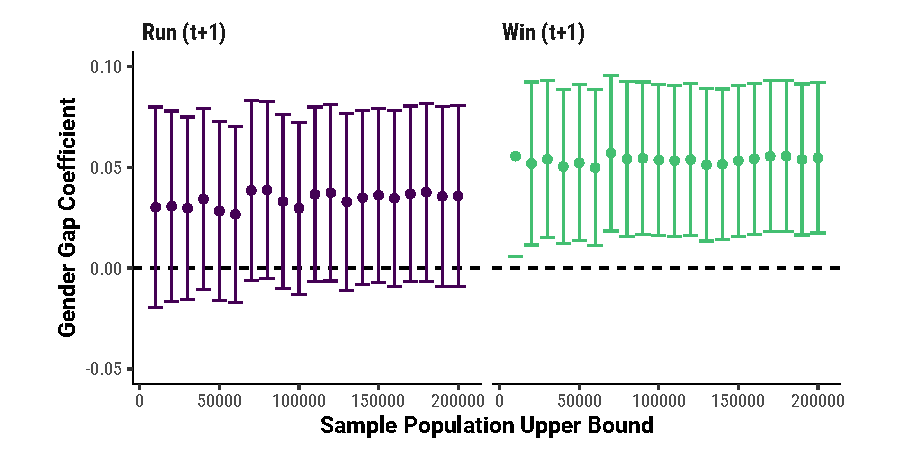
\includegraphics[width = 0.8 \textwidth]{../output/figures/spain_muni_robust.pdf}
    \caption{\textbf{Gender Gap in Incumbency Effect, Spain, By Maximum Municipality Size Included.}}
    \label{fig:spain_outliers}
\end{figure}


\subsubsection{Effect Magnitude By Population Tercile}

\begin{figure}[!htb]
    \centering
    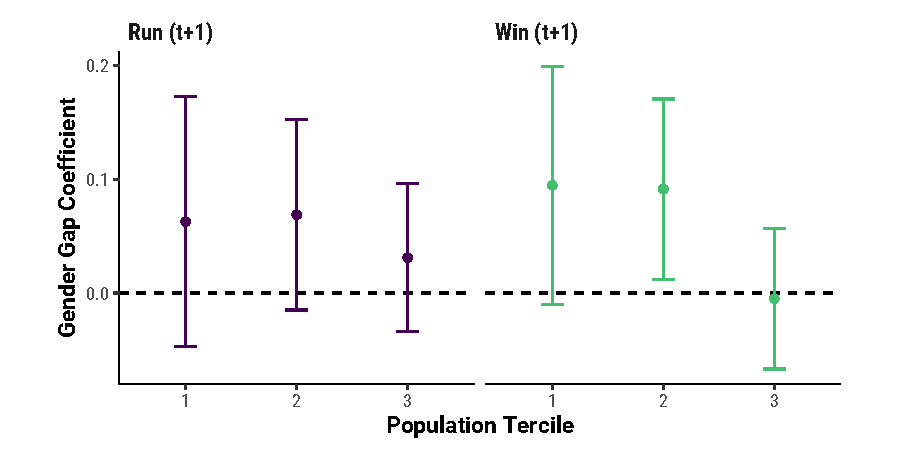
\includegraphics[width = 0.8 \textwidth]{../output/figures/spain_tercile_robust.pdf}
    \caption{\textbf{Gender Gap in Incumbency Effect, Spain, By Population Tercile.}}
    \label{fig:spain_tercile_robust}
\end{figure}


% \clearpage
% \section{Additional Statistical Results: Poland}
% \label{app:poland}

% In this section, I report additional results from the heterogeneity-in-discontinuity specification fitted on open-list PR, county-level elections in Poland.


\clearpage
\section{Descriptive Statistics}
\label{app:descriptive_statistics}

In this section, I report key summary statistics for both cases.

\begin{table}

\caption{Summary Statistics For Borderline Sample, Norway.}
\centering
\begin{tabular}[t]{lrrrr}
\toprule
  & Mean & SD & Min & Max\\
\midrule
Share Female & 0.39 & 0.49 & 0.00 & 1.00\\
Elected & 0.49 & 0.50 & 0.00 & 1.00\\
Population & 13254.37 & 21915.85 & 214.00 & 244620.00\\
Total Seats & 28.19 & 10.57 & 11.00 & 85.00\\
Running (t+1) & 0.56 & 0.50 & 0.00 & 1.00\\
Winning (t+1) & 0.26 & 0.44 & 0.00 & 1.00\\
\bottomrule
\end{tabular}
\end{table}


\begin{table}

\caption{Summary Statistics For Borderline Sample, Spain.}
\centering
\begin{tabular}[t]{lrrrr}
\toprule
  & Mean <- mean & SD <- sd & Min <- min & Max <- max\\
\midrule
Share Female & 0.38 & 0.48 & 0.00 & 1.00\\
Elected & 0.50 & 0.50 & 0.00 & 1.00\\
Population & 12070.60 & 26552.11 & 251.00 & 248150.00\\
Total Seats & 12.56 & 5.27 & 7.00 & 27.00\\
Running (t+1) & 0.49 & 0.50 & 0.00 & 1.00\\
Winning (t+1) & 0.25 & 0.44 & 0.00 & 1.00\\
\bottomrule
\end{tabular}
\end{table}


\clearpage
\section{Full Model Results}
\label{app:full_models}

In this section, I report results from the main paper including all coefficients in the specification.

\subsection{Norway}

\begin{table}[!h]

\caption{\label{tab:norway_main_full} \textbf{Difference-in-Discontinuity Estimates For Incumbency Advantage In Norwegian Municipalities.} Women face diminished incumbency effect on winning again.}
\centering
\fontsize{9}{11}\selectfont
\begin{threeparttable}
\begin{tabular}[t]{lS[
              input-symbols=(),
              table-format=-1.3,
              table-space-text-pre    = (,
              table-space-text-post   = ),
              input-open-uncertainty  =,
              input-close-uncertainty = ,
              table-align-text-post = false]S[
              input-symbols=(),
              table-format=-1.3,
              table-space-text-pre    = (,
              table-space-text-post   = ),
              input-open-uncertainty  =,
              input-close-uncertainty = ,
              table-align-text-post = false]S[
              input-symbols=(),
              table-format=-1.3,
              table-space-text-pre    = (,
              table-space-text-post   = ),
              input-open-uncertainty  =,
              input-close-uncertainty = ,
              table-align-text-post = false]S[
              input-symbols=(),
              table-format=-1.3,
              table-space-text-pre    = (,
              table-space-text-post   = ),
              input-open-uncertainty  =,
              input-close-uncertainty = ,
              table-align-text-post = false]S[
              input-symbols=(),
              table-format=-1.3,
              table-space-text-pre    = (,
              table-space-text-post   = ),
              input-open-uncertainty  =,
              input-close-uncertainty = ,
              table-align-text-post = false]S[
              input-symbols=(),
              table-format=-1.3,
              table-space-text-pre    = (,
              table-space-text-post   = ),
              input-open-uncertainty  =,
              input-close-uncertainty = ,
              table-align-text-post = false]}
\toprule
\multicolumn{1}{c}{ } & \multicolumn{3}{c}{Run (t + 1)} & \multicolumn{3}{c}{Win (t + 1)} \\
\cmidrule(l{3pt}r{3pt}){2-4} \cmidrule(l{3pt}r{3pt}){5-7}
  & \multicolumn{1}{c}{(1)} & \multicolumn{1}{c}{(2)} & \multicolumn{1}{c}{(3)} & \multicolumn{1}{c}{(4)} & \multicolumn{1}{c}{(5)} & \multicolumn{1}{c}{(6)}\\
\midrule
Elected & 0.002 & -0.010 & 0.016 & 0.107 & 0.102 & 0.109\\
 & (0.019) & (0.016) & (0.024) & (0.017) & (0.015) & (0.021)\\
\addlinespace
Female & -0.097 & -0.092 & -0.085 & -0.027 & -0.024 & -0.026\\
 & (0.021) & (0.018) & (0.026) & (0.018) & (0.015) & (0.021)\\
\addlinespace
Elected x Female & 0.002 & 0.024 & -0.030 & -0.062 & -0.047 & -0.096\\
 & (0.033) & (0.028) & (0.039) & (0.028) & (0.024) & (0.034)\\
\addlinespace \midrule \addlinespace
Margin & -1.255 & -0.615 & -2.168 & -0.668 & -0.106 & -0.686\\
 & (0.679) & (0.315) & (1.367) & (0.585) & (0.272) & (1.310)\\
Margin x Elected & 2.008 & 1.814 & 1.718 & 1.594 & 1.053 & 0.976\\
 & (0.979) & (0.450) & (2.031) & (0.881) & (0.436) & (2.068)\\
Margin x Female & -1.083 & -0.620 & 0.367 & 0.390 & 0.299 & 1.191\\
 & (1.029) & (0.477) & (2.021) & (0.871) & (0.400) & (1.896)\\
Margin x Elected x Female & 2.713 & -0.103 & 3.852 & 1.145 & -0.327 & 5.438\\
 & (1.377) & (0.709) & (2.853) & (1.279) & (0.653) & (3.045)\\
\addlinespace \midrule \addlinespace
Bandwidth & 0.054 & 0.11 & 0.027 & 0.05 & 0.099 & 0.025\\
BW Type & \multicolumn{1}{c}{Optimal} & \multicolumn{1}{c}{2x Opt} & \multicolumn{1}{c}{0.5x Opt} & \multicolumn{1}{c}{Optimal} & \multicolumn{1}{c}{2x Opt} & \multicolumn{1}{c}{0.5x Opt}\\
Outcome Mean & 0.564 & 0.575 & 0.551 & 0.261 & 0.263 & 0.257\\
N (left) & \multicolumn{1}{c}{4617} & \multicolumn{1}{c}{5529} & \multicolumn{1}{c}{3667} & \multicolumn{1}{c}{4502} & \multicolumn{1}{c}{5428} & \multicolumn{1}{c}{3549}\\
N (right) & \multicolumn{1}{c}{4666} & \multicolumn{1}{c}{5590} & \multicolumn{1}{c}{3711} & \multicolumn{1}{c}{4551} & \multicolumn{1}{c}{5489} & \multicolumn{1}{c}{3592}\\
\bottomrule
\end{tabular}
\begin{tablenotes}[para]
\item All estimates are reported with robust standard errors clustered at the municipality level in parentheses. Each observation is a candidate's election attempt. 'Elected' is an indicator for observations where the candidate obtained a seat in the municipal council. 'Female' is an indicator for observations identified as female. `Elected` times `Female` is the interaction between the two variables. Regression run on all candidates in elections between 2003 and 2015.
\end{tablenotes}
\end{threeparttable}
\end{table}

\clearpage
\subsection{Spain}

\begin{table}[!h]

\caption{\label{tab:spain_main_full} \textbf{Difference-in-Discontinuity Estimates For Incumbency Advantage In Spanish Municipalities}. Women likely enjoy a larger effect of winning on their probability to win again.}
\centering
\fontsize{9}{11}\selectfont
\begin{threeparttable}
\begin{tabular}[t]{lS[
              input-symbols=(),
              table-format=-1.3,
              table-space-text-pre    = (,
              table-space-text-post   = ),
              input-open-uncertainty  =,
              input-close-uncertainty = ,
              table-align-text-post = false]S[
              input-symbols=(),
              table-format=-1.3,
              table-space-text-pre    = (,
              table-space-text-post   = ),
              input-open-uncertainty  =,
              input-close-uncertainty = ,
              table-align-text-post = false]S[
              input-symbols=(),
              table-format=-1.3,
              table-space-text-pre    = (,
              table-space-text-post   = ),
              input-open-uncertainty  =,
              input-close-uncertainty = ,
              table-align-text-post = false]S[
              input-symbols=(),
              table-format=-1.3,
              table-space-text-pre    = (,
              table-space-text-post   = ),
              input-open-uncertainty  =,
              input-close-uncertainty = ,
              table-align-text-post = false]S[
              input-symbols=(),
              table-format=-1.3,
              table-space-text-pre    = (,
              table-space-text-post   = ),
              input-open-uncertainty  =,
              input-close-uncertainty = ,
              table-align-text-post = false]S[
              input-symbols=(),
              table-format=-1.3,
              table-space-text-pre    = (,
              table-space-text-post   = ),
              input-open-uncertainty  =,
              input-close-uncertainty = ,
              table-align-text-post = false]}
\toprule
\multicolumn{1}{c}{ } & \multicolumn{3}{c}{Run (t + 1)} & \multicolumn{3}{c}{Win (t + 1)} \\
\cmidrule(l{3pt}r{3pt}){2-4} \cmidrule(l{3pt}r{3pt}){5-7}
  & \multicolumn{1}{c}{(1)} & \multicolumn{1}{c}{(2)} & \multicolumn{1}{c}{(3)} & \multicolumn{1}{c}{(4)} & \multicolumn{1}{c}{(5)} & \multicolumn{1}{c}{(6)}\\
\midrule
Elected & 0.109 & 0.119 & 0.100 & 0.072 & 0.095 & 0.076\\
 & (0.014) & (0.010) & (0.020) & (0.012) & (0.008) & (0.017)\\
\addlinespace
Female & -0.024 & -0.032 & -0.012 & -0.032 & -0.026 & -0.033\\
 & (0.016) & (0.012) & (0.022) & (0.013) & (0.009) & (0.018)\\
\addlinespace
Elected x Female & 0.037 & 0.033 & 0.018 & 0.058 & 0.045 & 0.057\\
 & (0.023) & (0.017) & (0.032) & (0.019) & (0.013) & (0.027)\\
\addlinespace \midrule \addlinespace
Margin & 0.538 & 0.537 & 3.069 & 1.346 & 1.005 & 1.870\\
 & (0.570) & (0.212) & (1.558) & (0.390) & (0.144) & (1.130)\\
Margin x Elected & 0.197 & -0.633 & -3.674 & 0.389 & -0.596 & -1.254\\
 & (0.799) & (0.301) & (2.195) & (0.594) & (0.224) & (1.669)\\
Margin x Female & 0.358 & -0.273 & 2.509 & -0.913 & -0.415 & -0.914\\
 & (0.912) & (0.339) & (2.416) & (0.627) & (0.228) & (1.741)\\
Margin x Elected x Female & -1.841 & -0.239 & -2.296 & -0.404 & -0.329 & -0.241\\
 & (1.282) & (0.483) & (3.405) & (0.958) & (0.362) & (2.701)\\
\addlinespace \midrule \addlinespace
Bandwidth & 0.032 & 0.064 & 0.016 & 0.035 & 0.071 & 0.018\\
BW Type & \multicolumn{1}{c}{Optimal} & \multicolumn{1}{c}{2x Opt} & \multicolumn{1}{c}{0.5x Opt} & \multicolumn{1}{c}{Optimal} & \multicolumn{1}{c}{2x Opt} & \multicolumn{1}{c}{0.5x Opt}\\
Outcome Mean & 0.486 & 0.483 & 0.485 & 0.256 & 0.251 & 0.254\\
N (left) & \multicolumn{1}{c}{14840} & \multicolumn{1}{c}{26294} & \multicolumn{1}{c}{7984} & \multicolumn{1}{c}{16223} & \multicolumn{1}{c}{28426} & \multicolumn{1}{c}{8726}\\
N (right) & \multicolumn{1}{c}{14729} & \multicolumn{1}{c}{26886} & \multicolumn{1}{c}{7825} & \multicolumn{1}{c}{16159} & \multicolumn{1}{c}{29072} & \multicolumn{1}{c}{8530}\\
\bottomrule
\end{tabular}
\begin{tablenotes}[para]
\item All estimates are reported with robust standard errors clustered at the municipality level in parentheses. See Table 2 for additional details.
\end{tablenotes}
\end{threeparttable}
\end{table}

\clearpage
\subsection{Norway, By Party Group}

\begin{table}[!h]

\caption{\label{tab:norway_by_party_inc_full} \textbf{Difference-in-Discontinuity Estimates For Incumbency Advantage In Norwegian Municipalities, By Political Party Group.}}
\centering
\fontsize{9}{11}\selectfont
\begin{threeparttable}
\begin{tabular}[t]{lS[
              input-symbols=(),
              table-format=-2.3,
              table-space-text-pre    = (,
              table-space-text-post   = ),
              input-open-uncertainty  =,
              input-close-uncertainty = ,
              table-align-text-post = false]S[
              input-symbols=(),
              table-format=-2.3,
              table-space-text-pre    = (,
              table-space-text-post   = ),
              input-open-uncertainty  =,
              input-close-uncertainty = ,
              table-align-text-post = false]S[
              input-symbols=(),
              table-format=-2.3,
              table-space-text-pre    = (,
              table-space-text-post   = ),
              input-open-uncertainty  =,
              input-close-uncertainty = ,
              table-align-text-post = false]S[
              input-symbols=(),
              table-format=-2.3,
              table-space-text-pre    = (,
              table-space-text-post   = ),
              input-open-uncertainty  =,
              input-close-uncertainty = ,
              table-align-text-post = false]}
\toprule
\multicolumn{1}{c}{ } & \multicolumn{2}{c}{Run (t+1)} & \multicolumn{2}{c}{Win (t+1)} \\
\cmidrule(l{3pt}r{3pt}){2-3} \cmidrule(l{3pt}r{3pt}){4-5}
  & \multicolumn{1}{c}{(1)} & \multicolumn{1}{c}{(2)} & \multicolumn{1}{c}{(3)} & \multicolumn{1}{c}{(4)}\\
\midrule
Elected & 0.022 & 0.005 & 0.086 & 0.126\\
 & (0.031) & (0.026) & (0.027) & (0.024)\\
\addlinespace
Female & -0.079 & -0.044 & -0.015 & -0.001\\
 & (0.034) & (0.030) & (0.027) & (0.025)\\
\addlinespace
Elected x Female & -0.040 & -0.014 & -0.053 & -0.089\\
 & (0.049) & (0.045) & (0.039) & (0.039)\\
\addlinespace \midrule \addlinespace
Margin & -0.583 & -1.690 & -0.499 & -0.491\\
 & (1.362) & (0.627) & (1.082) & (0.519)\\
Margin x Elected & -1.242 & 3.626 & 1.511 & 1.713\\
 & (1.931) & (0.878) & (1.664) & (0.799)\\
Margin x Female & 0.237 & 0.532 & 1.501 & -0.038\\
 & (1.902) & (1.069) & (1.521) & (0.911)\\
Margin x Elected x Female & 3.353 & -1.834 & -1.126 & 0.412\\
 & (2.604) & (1.506) & (2.369) & (1.351)\\
\addlinespace \midrule \addlinespace
Parties & \multicolumn{1}{c}{Left} & \multicolumn{1}{c}{Right} & \multicolumn{1}{c}{Left} & \multicolumn{1}{c}{Right}\\
Bandwidth & 0.05 & 0.068 & 0.052 & 0.069\\
Outcome Mean & 0.546 & 0.59 & 0.253 & 0.26\\
N (left) & \multicolumn{1}{c}{1568} & \multicolumn{1}{c}{2382} & \multicolumn{1}{c}{1580} & \multicolumn{1}{c}{2388}\\
N (right) & \multicolumn{1}{c}{1589} & \multicolumn{1}{c}{2413} & \multicolumn{1}{c}{1601} & \multicolumn{1}{c}{2419}\\
\bottomrule
\end{tabular}
\begin{tablenotes}[para]
\item All estimates are reported with robust standard errors clustered at the municipality level in parentheses. Each observation is a candidate's election attempt.
\end{tablenotes}
\end{threeparttable}
\end{table}

\clearpage
\subsection{Norway, Mechanisms}

\begin{table}[!h]

\caption{\label{tab:norway_by_party_mech_full} \textbf{Mechanisms leading to lower incumbency advantage: Difference-in-Discontinuity Estimates On Additional Outcomes, Norway.}}
\centering
\fontsize{9}{11}\selectfont
\begin{threeparttable}
\begin{tabular}[t]{lS[
              input-symbols=(),
              table-format=-2.3,
              table-space-text-pre    = (,
              table-space-text-post   = ),
              input-open-uncertainty  =,
              input-close-uncertainty = ,
              table-align-text-post = false]S[
              input-symbols=(),
              table-format=-2.3,
              table-space-text-pre    = (,
              table-space-text-post   = ),
              input-open-uncertainty  =,
              input-close-uncertainty = ,
              table-align-text-post = false]S[
              input-symbols=(),
              table-format=-2.3,
              table-space-text-pre    = (,
              table-space-text-post   = ),
              input-open-uncertainty  =,
              input-close-uncertainty = ,
              table-align-text-post = false]S[
              input-symbols=(),
              table-format=-2.3,
              table-space-text-pre    = (,
              table-space-text-post   = ),
              input-open-uncertainty  =,
              input-close-uncertainty = ,
              table-align-text-post = false]S[
              input-symbols=(),
              table-format=-2.3,
              table-space-text-pre    = (,
              table-space-text-post   = ),
              input-open-uncertainty  =,
              input-close-uncertainty = ,
              table-align-text-post = false]S[
              input-symbols=(),
              table-format=-2.3,
              table-space-text-pre    = (,
              table-space-text-post   = ),
              input-open-uncertainty  =,
              input-close-uncertainty = ,
              table-align-text-post = false]S[
              input-symbols=(),
              table-format=-2.3,
              table-space-text-pre    = (,
              table-space-text-post   = ),
              input-open-uncertainty  =,
              input-close-uncertainty = ,
              table-align-text-post = false]S[
              input-symbols=(),
              table-format=-2.3,
              table-space-text-pre    = (,
              table-space-text-post   = ),
              input-open-uncertainty  =,
              input-close-uncertainty = ,
              table-align-text-post = false]}
\toprule
\multicolumn{1}{c}{ } & \multicolumn{2}{c}{Orig. Rank Advance} & \multicolumn{2}{c}{Actual Rank Advance} & \multicolumn{2}{c}{Pre-Ad. (t+1)} & \multicolumn{2}{c}{Pers.V. Share (t+1)} \\
\cmidrule(l{3pt}r{3pt}){2-3} \cmidrule(l{3pt}r{3pt}){4-5} \cmidrule(l{3pt}r{3pt}){6-7} \cmidrule(l{3pt}r{3pt}){8-9}
  & \multicolumn{1}{c}{(1)} & \multicolumn{1}{c}{(2)} & \multicolumn{1}{c}{(3)} & \multicolumn{1}{c}{(4)} & \multicolumn{1}{c}{(5)} & \multicolumn{1}{c}{(6)} & \multicolumn{1}{c}{(7)} & \multicolumn{1}{c}{(8)}\\
\midrule
Elected & 0.088 & 0.066 & 0.026 & 0.044 & 0.037 & 0.058 & 0.003 & 0.005\\
 & (0.026) & (0.020) & (0.028) & (0.021) & (0.019) & (0.019) & (0.002) & (0.001)\\
\addlinespace
Female & 0.003 & -0.003 & -0.031 & 0.011 & 0.017 & 0.049 & -0.003 & 0.000\\
 & (0.027) & (0.023) & (0.029) & (0.023) & (0.022) & (0.021) & (0.003) & (0.002)\\
\addlinespace
Elected x Female & -0.063 & -0.034 & -0.013 & -0.062 & 0.001 & -0.041 & 0.001 & -0.005\\
 & (0.038) & (0.034) & (0.039) & (0.032) & (0.031) & (0.033) & (0.004) & (0.003)\\
\addlinespace \midrule \addlinespace
Margin & -0.572 & -0.352 & 0.611 & 0.006 & -2.940 & -1.802 & -0.593 & -0.254\\
 & (0.908) & (0.386) & (0.922) & (0.348) & (1.303) & (0.554) & (0.198) & (0.142)\\
Margin x Elected & -1.586 & -0.511 & -2.806 & -0.853 & 6.176 & 4.371 & 1.875 & 0.584\\
 & (1.222) & (0.636) & (1.242) & (0.520) & (2.035) & (0.921) & (0.393) & (0.309)\\
Margin x Female & 0.705 & 1.088 & -0.023 & 0.794 & 0.722 & 0.499 & -0.931 & 0.097\\
 & (1.287) & (0.660) & (1.358) & (0.570) & (2.147) & (1.002) & (0.794) & (0.162)\\
Margin x Elected x Female & 1.813 & -1.590 & 2.354 & -0.772 & -1.676 & -0.181 & 0.646 & 0.014\\
 & (1.687) & (0.969) & (1.937) & (0.797) & (3.104) & (1.501) & (0.881) & (0.371)\\
\addlinespace \midrule \addlinespace
Parties & \multicolumn{1}{c}{Left} & \multicolumn{1}{c}{Right} & \multicolumn{1}{c}{Left} & \multicolumn{1}{c}{Right} & \multicolumn{1}{c}{Left} & \multicolumn{1}{c}{Right} & \multicolumn{1}{c}{Left} & \multicolumn{1}{c}{Right}\\
Bandwidth & 0.068 & 0.092 & 0.061 & 0.097 & 0.033 & 0.055 & 0.025 & 0.052\\
Outcome Mean & 0.257 & 0.253 & 0.229 & 0.211 & 0.119 & 0.163 & 0.0204 & 0.0175\\
N (left) & \multicolumn{1}{c}{1655} & \multicolumn{1}{c}{2620} & \multicolumn{1}{c}{1624} & \multicolumn{1}{c}{2662} & \multicolumn{1}{c}{1421} & \multicolumn{1}{c}{2203} & \multicolumn{1}{c}{446} & \multicolumn{1}{c}{840}\\
N (right) & \multicolumn{1}{c}{1676} & \multicolumn{1}{c}{2655} & \multicolumn{1}{c}{1645} & \multicolumn{1}{c}{2698} & \multicolumn{1}{c}{1441} & \multicolumn{1}{c}{2229} & \multicolumn{1}{c}{458} & \multicolumn{1}{c}{856}\\
\bottomrule
\end{tabular}
\begin{tablenotes}[para]
\item All estimates are reported with robust standard errors clustered at the municipality level in parentheses. Each observation is a candidate's election attempt.
\end{tablenotes}
\end{threeparttable}
\end{table}

\end{document}
